\documentclass[11pt, twoside, a4paper]{book}

\newcommand\authorname{Juan Carlos PRIETO}	% Pensez a mettre votre nom ici

\usepackage[english]{babel}
\usepackage[utf8]{inputenc}
\usepackage[T1]{fontenc}
\usepackage{lmodern}
\usepackage{vmargin} 
\usepackage{indentfirst} 
\usepackage{textcomp}
\usepackage{setspace}
\usepackage{soul}
\usepackage{longtable}
\usepackage{array}

\usepackage{cite}
\usepackage{epsfig}
\usepackage{subfigure}
\usepackage{wrapfig}
\usepackage{calc}
\usepackage{amssymb}
\usepackage{amstext}
\usepackage{amsmath}
\usepackage{amsthm}
\usepackage{multicol}
\usepackage{multirow}
\usepackage{url}
\usepackage{hyperref} 
\usepackage{enumerate}

\newtheorem{definition}{Definition}

\graphicspath{{./logo/}{./data/eps/}}

\makeatletter
\renewcommand{\@chapapp}{}% Not necessary...
\newenvironment{chapquote}[2][2em]
  {\setlength{\@tempdima}{#1}%
   \def\chapquote@author{#2}%
   \parshape 1 \@tempdima \dimexpr\textwidth-2\@tempdima\relax%
   \itshape}
  {\par\normalfont\hfill--\ \chapquote@author\hspace*{\@tempdima}\par\bigskip}
\makeatother


\usepackage{fancyhdr}


%\usepackage{inputs/thesisCreatis}

\begin{document}
\sloppy
\pagenumbering{roman}

\frontmatter
% D�finition de la page de garde
\clearpage

% *************** Front matter ***************
% *************** Title page ***************
\pagestyle{empty}
\thispagestyle{empty} \noindent 


%%%% debut macro %%%%
\newenvironment{changemargin}[2]{\begin{list}{}{%
\setlength{\topsep}{0pt}%
\setlength{\leftmargin}{0pt}%
\setlength{\rightmargin}{0pt}%
\setlength{\listparindent}{\parindent}%
\setlength{\itemindent}{\parindent}%
\setlength{\parsep}{0pt plus 1pt}%
\addtolength{\leftmargin}{#1}%
\addtolength{\rightmargin}{#2}%
}\item }{\end{list}}
%%%% fin macro %%%%

\begin{changemargin}{-1.7cm}{0 cm}

%\newcolumntype{M}[1]{>{\raggedright}m{#1}}
\begin{tabular}{l m{5cm} c m{5cm} r m{5cm}}

\includegraphics[height= 2cm]{UdL.eps} &  & 
\includegraphics[height= 2cm]{INSA.eps} \\
  &   &  \\
  &   &  \\
\small Num\'ero d'ordre : ISAL 0010 &   & \small Ann\'ee 2014
\end{tabular}

\vspace{0.6cm}

\begin{center}
{\Large TH\`ESE}

\vspace{0.15cm}

{D\'{e}livr\'{e}e par}

\vspace{0.15cm}

{\Large L'Insitut National des Sciences Appliqu\'ees de Lyon}

\vspace{0.5cm}

{\Large DIPL\^{O}ME DE DOCTORAT}

\vspace{0.15cm}

{(arr\^{e}t\'{e} du 7 aout 2006)}

\vspace{0.5cm}

{\Large \'ECOLE DOCTORALE : \'{E}lectronique, \'{E}lectrotechnique,
Automatique
Sp\'{e}cialit\'e: STIC Sant\'{e}
}

\vspace{0.5cm}

{Soutenue publiquement le 31 Janvier 2014 par}

\vspace{0.25cm}

{\Large \authorname}

\vspace{0.25cm}

\Huge \bf Multiparametric organ modeling for shape statistics and simulation procedures.

\vspace{0.3cm}
\end{center}


\begin{center}
{\Large Jury} \\
\vspace{0.5cm}
\begin{tabular}{lll}
    {\bf Christophe ODET} & Professeur, INSA - Lyon & Directeur de th\`{e}se \\
    {\bf Chantal MULLER} & Maitre de Conf\'{e}rences, INSA - Lyon & Co-directeur de th\`{e}se \\
    {\bf Martin STYNER}   & Maitre de Conf\'{e}rences, NIRAL - UNC & Rapporteur \\
    {\bf Christian GERMAIN} & Professeur,  IMS - Universit\'{e} Bordeaux & Rapporteur \\
    {\bf David ROUSSEAU}   & Professeur,  INSA - Lyon & Examinateur \\
    {\bf Fran\c{c}ois COTTON} & Professeur, Centre Hospitalier Lyon-Sud & Examinateur \\
    {\bf Charles GUTTMANN}   & Maitre de Conf\'{e}rences, BWH - Boston Massachusetts & Examinateur \\
    {\bf Stephen PIZER}   & Professeur, MIDAG - UNC & Examinateur \\
\end{tabular}
\end{center}

\end{changemargin}



% Remerciements
\input{inputs/ack}

% Abstract
% ********** Abstract **********
\cleardoublepage

\section*{\huge Abstract}
\addcontentsline{toc}{chapter}{Abstract}

Geometric modeling has been one of the most researched areas 
in the medical domain.
Today, there is not a well established methodology to model the shape of an organ. 
There are many approaches available and each one of them have different strengths and weaknesses.

Most state of the art methods to model shape use surface information only.
There is an increasing need for techniques to support volumetric information.
Besides shape characterization, a technique to differentiate objects by shape is needed.
This requires computing statistics on shape.

%The current challenge of research in life sciences is to create
%models to represent the surface, the interior of an object,
%and give statistical differences based on shape.

In this work, we use a technique for shape modeling that is
able to model surface and internal features, and 
is suited to compute shape statistics.

Using this technique (s-rep), a procedure to model the human cerebral cortex is proposed. 
This novel representation offers new possibilities to analyze cortical lesions
and compute shape statistics on the cortex.

The second part of this work proposes a methodology to 
parameterize the interior of an object.
The method is flexible and can 
enhance the visual aspect or the description of physical properties of an object.

The geometric modeling enhanced with physical parameters is used 
to produce simulated magnetic resonance images.
This image simulation approach is validated by analyzing the behavior and performance of classic segmentation algorithms for real images.


% ********** Abstract **********
\newpage
\section*{\huge Résumé}

La modélisation géométrique a été l'un des sujets les plus étudiés pour la représentation des structures anatomiques dans le domaine médical.
Aujourd'hui, il n'y a toujours pas de méthode bien établie pour modéliser la forme d'un organe.
Cependant, il y a plusieurs types d'approches disponibles et chaque approche a ses forces et ses faiblesses.

La plupart des méthodes de pointe utilisent uniquement l'information surfacique mais
un besoin croissant de modéliser l'information volumique des objets apparaît.
En plus de la description géométrique, il faut pouvoir différencier les objets d'une population selon leur forme.
Cela nécessite de disposer des statistiques sur la forme dans organe dans une population donné.

Dans ce travail de thèse, on utilise une représentation capable de modéliser les caractéristiques surfaciques et internes d'un objet.
La représentation choisie (s-rep) a en plus l'avantage de permettre de déterminer les statistiques de forme pour une population d'objets.

En s'appuyant sur cette représentation, une procédure pour modéliser le cortex cérébral humain est proposée.
Cette nouvelle modélisation offre de nouvelles possibilités pour analyser les lésions corticales
et calculer des statistiques de forme sur le cortex.

La deuxième partie de ce travail propose une méthodologie pour décrire de manière paramétrique l'intérieur d'un objet.
La méthode est flexible et peut améliorer l'aspect visuel ou la description des propriétés physiques d'un objet.

La modélisation géométrique enrichie avec des paramètres physiques volumiques
est utilisée pour la simulation d'image par résonance magnétique pour produire des simulations plus réalistes.
Cette approche de simulation d'images est validée en analysant le comportement et les performances des méthodes de segmentations
classiquement utilisées pour traiter des images réelles du cerveau.

% Definition de la table des mati�res
% \clearpage ~~~~ \thispagestyle{plain} \newpage\thispagestyle{plain}
\cleardoublepage
% \phantomsection
\listoffigures
\clearpage
\tableofcontents								% Cr�ation de la table des mati�res
\addcontentsline{toc}{chapter}{Contents}

% Liste des symboles
% *************** List of symbols and abbreviations ***************

% ******************************************************************************
% You can make list of symbols and abbreviations here.
% You only need to make a label when a symbol is introduced in the document and
% here you can reference this label to obtain page number.
% ******************************************************************************

\chapter*{Abbreviations}
\addcontentsline{toc}{chapter}{List of Symbols}

\begin{center}
\begin{tabular}{cp{12cm}}

$\mu$MR & Micro magnetic resonance \\
AAM & Active appereance models \\
ASM & Active shape models \\
b-reps & Boundary representations \\
CA  & Computational anatomy) \\
CT & Computed tomography \\
DT & Distance Transform \\
DTI & Diffusion tensor imaging \\
ET & Echo time \\
FEM & Finite element method \\
MA  & Medial axis \\
MAT & Medial axis transform \\
MRF & Markov Random Field \\
MRG & Model Guided Rendering \\
MRI & Magnetic resonance imaging \\
MS  & Medial axis or medial sheet\\
ODE & Ordinary differential equation \\
PDM & Point distrubution models \\
PCA & Principal component analysis\\
PET & Positron emission tomography)\\
RF  & Radio Frequency \\
SR$\mu$CT &  Synchrotron Radiation Computed Micro-Tomography \\
s-rep & Skeletal representation \\
SS  & Skeletal sheet \\
TR & Time repetition \\
US & Ultra sound \\ 

\end{tabular}
\end{center}

% *************** End of list of symbols and abbreviations ***************



%%%%%%%%%%%%%%%%%%%%%%%
%% MAIN
%%%%%%%%%%%%%%%%%%%%%%%
\mainmatter

\pagestyle{plain}
\cfoot{\thepage}

\pagenumbering{arabic}


\graphicspath{{Introduction/images/}}

\chapter{Introduction}
\label{chapter:Introduction}

Recent advances on digital imaging modalities
and computation have enabled an emerging field 
studying the biological variability of human anatomy. 
This field is called CA (computational anatomy).

CA as defined by \cite{Grenander1998} has three principal aspects: construction of
anatomical manifolds or shape modeling by points, curves, surfaces and volumes;
comparison of these models; and statistical analysis of shape variability.

The statistics allows for inference and hypothesis testing of disease states.
This is done using the statistical description
to determine the probability of a hypothesis to be true or false.
In other words, a new sample is classified as diseased or healthy 
according to its shape.

The automated construction of anatomical models 
has been the main interest of many research groups around the world. 
These models are based on algorithms and equations that capture the behavior
and/or the appearance of the object.

Besides hypothesis testing, the models are also used for 
various types of simulation procedures such as simulation of medical images.
Medical imaging consists in acquiring details of the interior of the human body by using different techniques. 
Among these techniques we find MRI (magnetic resonance imaging), CT (computed tomography),
US (ultrasound) or PET (positron emission tomography). 
They are widely used to diagnose and plan treatment for patients with the information acquired in the image.
These imaging devices can be very expensive, they require regular maintenance and are used only by specialized staff. 
In this context, image simulation is defined as the process of producing a synthesized image 
from a specific modality using the geometry of a virtual object. 
The virtual object in question could be an organ or a system of organs.

One purpose of image simulation is to improve imaging devices.
This is done by acquiring better understanding of image acquisition phenomena
or calibrating a specific set of parameters that will produce a desired outcome 
and then translate the experience to the real device.
Another use for simulated images is to evaluate the performance of segmentation algorithms as 
the results can be directly correlated to the virtual model.

Other types of simulations are done to understand biological process,
muscle deformation, cardiac cycle, respiratory cycle, cortical folding etc. 

Knowing all the potential applications on the medical domain,
the current challenge today is to create a virtual human, in other words,
to create a model capable of integrating anatomical, physiological, mechanical,  
biological and physical information. 
This virtual human could be used to improve simulation procedures
and also hypothesis testing for disease states. 

The first objective of this dissertation 
is to provide a technique generic enough to model
the shape of various organs, 
giving the possibility to include information 
from different spatial scales, imaging modalities or 
other sources.
To model the shape of an object, there are many approaches available.
Notably deformable models have proven to be successful. 
They are able to automate, to a certain degree, 
image segmentation of structures and they also produce statistics on the deformations. 
Unfortunately, some of the techniques 
don't provide the necessary mechanisms for further use on simulation procedures. 
Chapter \ref{chapter:3DModels} summarizes the important features of the techniques 
frequently used to model the geometry of objects.
The choice of the modeling technique should meet some specific requirements 
that will be used to model the human cerebral cortex. 
The representation should support the extremely 
folded geometry of the cortex
and also be capable to locate 
internal features or 
provide a sense of orientation at every place inside the object. 

Chapter \ref{chapter:cortexModeling} explains 
a methodology to create a cortex representation. 
The modeling technique relates to 
the true shape of the cortex which is that of a folded slab
as most of the state of the art methods only use surface information or 
model the folds locally. 

The second objective 
is to provide a mechanism
to synthesize solids, meaning 
surface and internal properties 
of the object must be available.
The procedure to synthesize solids uses small two dimensions
textured images as exemplars. The synthesized result is visually and statistically 
similar to the exemplar.
The textured images can be from various sources 
including images from the web, 
histology and complex ones such as 
MRI physical parameters acquired with relaxometry techniques.
The generated solids can be used
to enhance the visualization and/or internal properties of the models created
using the techniques described in Chapter \ref{chapter:3DModels}.
Chapter \ref{chapter:textureSynthesis} explains the solid synthesis procedure.

The third objective is to use
the geometric description enhanced 
with internal properties such as physical parameters
and generate simulated MRIs.
Chapter \ref{chapter:MRISimulation} explains MRI simulation and 
uses the techniques for geometric modeling and
solid synthesis to create some virtual objects.
These objects are used to simulate MRIs, which are
validated with well known segmentation algorithms. 

Chapter \ref{chapter:Conclusions} concludes the current research study 
and future perspectives are declared. 


\newpage
\input{ChapterSrep/ChapterSrep}

\graphicspath{{ChapterCortex/images/}}
%% Chapitre I %%
\chapter{Cortex modeling via s-reps}
\label{chapter:cortexModeling}

\section{Introduction}
\label{sec:Introduction}

The cerebral cortex is a highly folded slab of neural tissue 
with compact interconnections that enables sophisticated processing of information.
It plays an important role in memory, attention, perceptual awareness, thought, language, and consciousness.
Progress has been made in understanding the structure and function of the cortex.
\cite{lorente1934studies} proposed that the cortex is formed by small cylinders containing vertical chains of neurons; 
These structures were later called columns, corresponding to groups of local cells running perpendicular to the cortical surface.
This hypothesis was later confirmed with the physiological studies done by \cite{mountcastle1998perceptual}. 

The cortex is a layered sheet with a more or less uniform cellular structure. 
It is composed by the following layers:
\begin{enumerate}
 \item Layer I (molecular layer): apical dendrites of cells and axons; 
 \item Layer II (external granular layer): small granule cells and some larger pyramidal cells;
 \item Layer III (external pyramidal layer): small to medium sized pyramidal neurons;
 \item Layer IV (Internal granular layer): interneurons receiving ascending sensory input and projecting to layers II/III. No pyramidal neurons are found in this layer;
 \item Layer V (Internal pyramidal layer): medium to very large pyramidal neurons; 
 \item Layer VI (Multiform layer): assortment of cell types including pyramidal cells, cells that receive input from layers II, III and V and 
       axons projecting to superficial cortical layers and subcortical regions.
\end{enumerate}
Today the columnar organization is the most widely adopted model to explain the cortical processing of information.

\begin{figure}[htb]
 \centering 
    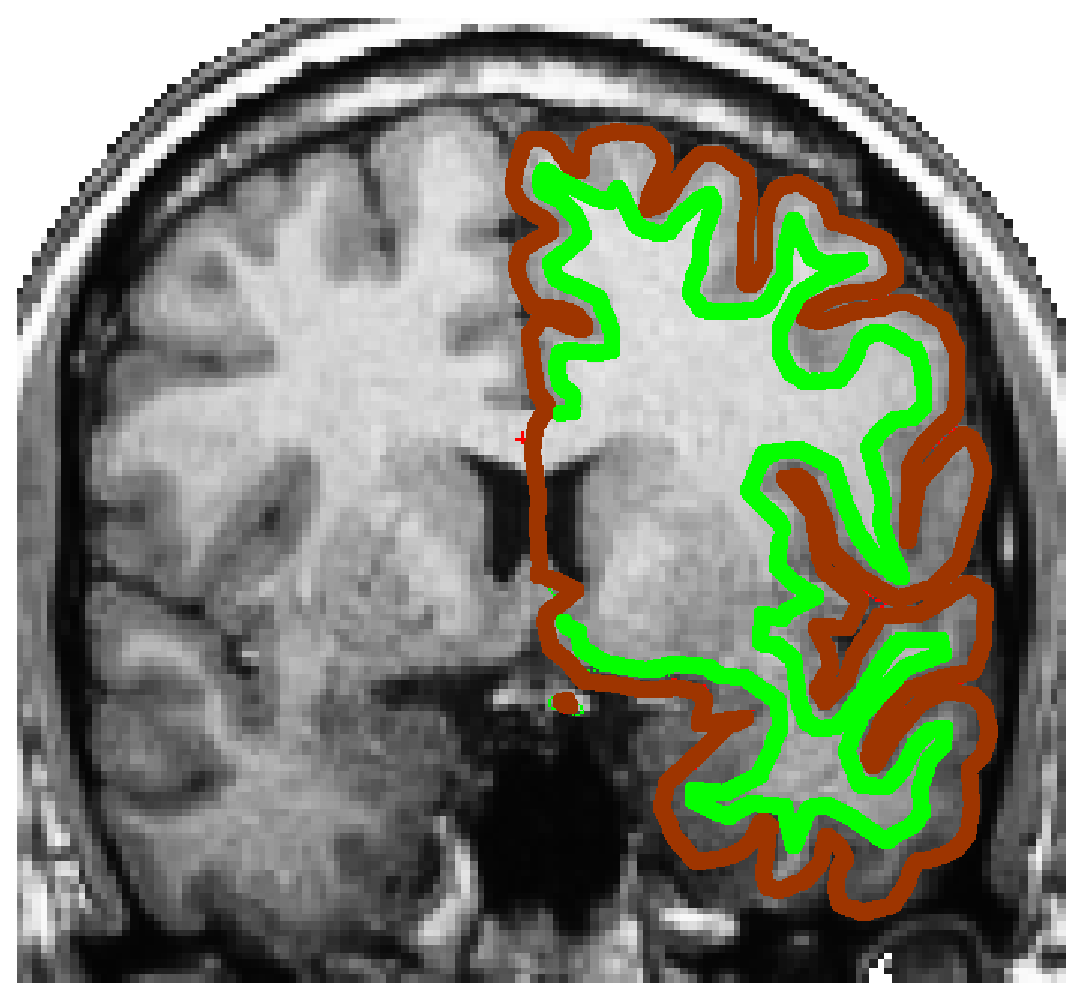
\epsfig{file = lh_BrainFreesurfer.eps, width = 8cm}
 \caption[Brain MRI.]{Brain MRI. The grey and white matter surfaces are shown in brown and green respectively.}
 \label{fig:MRIimage}  
\end{figure}

Figure \ref{fig:MRIimage} shows a slice of an MRI with the cortex region outlined. In brown the grey matter (GM) and in green the white matter (WM) surfaces are shown.
Since nearly two thirds of the cortical surface is buried within the sulci, it is difficult to perform computation and visualization tasks. 
Different procedures have been developed to unfold and map the cortical surface onto different spaces (inflated, spherical or flattened)
\cite{drury_computerized_1996}, \cite{hermosillo_unfolding_1999}, \cite{fischl_cortical_1999}, \cite{pons_area_2004}. 
This allows the cortical surface to be analyzed and visualized and statistical methods to be applied on these spaces.
\textit{Freesurfer} (an automated tool for brain's cortical surface reconstruction using structural MRI data)
uses the inflation and flattening procedure from \cite{fischl_cortical_1999}. 

Likewise, cortex evolution has also been a subject of great interest.
Much of the efforts have been focused on understanding how the folding process occurs.
Many species have folded cortices, but the degree of folding is different among them.
In general terms, a greater degree of folding is related to higher intelligence \cite{buettner1964evolutionary}.
Humans have extremely folded cortices.
%how this process occurs is not clearly understood. 
The folding patterns are 
unique to each brain, and abnormal folding is related to 
neurological disorders such as schizophrenia, epilepsy, autism and Down's syndrome.
Different methods have been proposed to explain how the folding occurs: 
growing a 2D curve in a closed space \cite{raghavan1997continuum}; 
growing 2D and 3D truss elements constrained by radially aligned fibers \cite{toro2005morphogenetic}; 
using spherical wavelets on close surfaces \cite{yu2007cortical}; 
using a FEM (finite element method) biomechanical model \cite{geng2009biomechanisms};
combining a mathematical model with biomechanical data \cite{bayly2013mechanical}.
For a recent review on folding theories see \cite{filas2013mechanisms}.

There are research opportunities in developing cortex models. 
As stated by Javier de Felipe \cite{defelipe2012neocortical}, ``it is still necessary
to achieve a better fundamental understanding of what columns
are and how they are used in cortical processes. Accordingly, it
is now important to translate recent technical advances and
new findings in the neurosciences into practical applications for
neuroscientists, clinicians, and for those interested in comparative
anatomy and brain evolution.''

Taking these facts into consideration, one of the objectives in this dissertation is to provide a
tool that models the shape of the cortex and relates to the real physical structure. 
Section \ref{sec:s-repImplementation} defines an s-rep
with the corresponding interpolation mechanisms that parameterize the interior of the object by $[u, v, \tau]$.
S-reps can be used to model the anatomic and physiologic information from the different layers of the cortex.
This information can be naturally included using the $\tau$ coordinate.

\begin{figure} 
 \centering 
	\subfigure[]{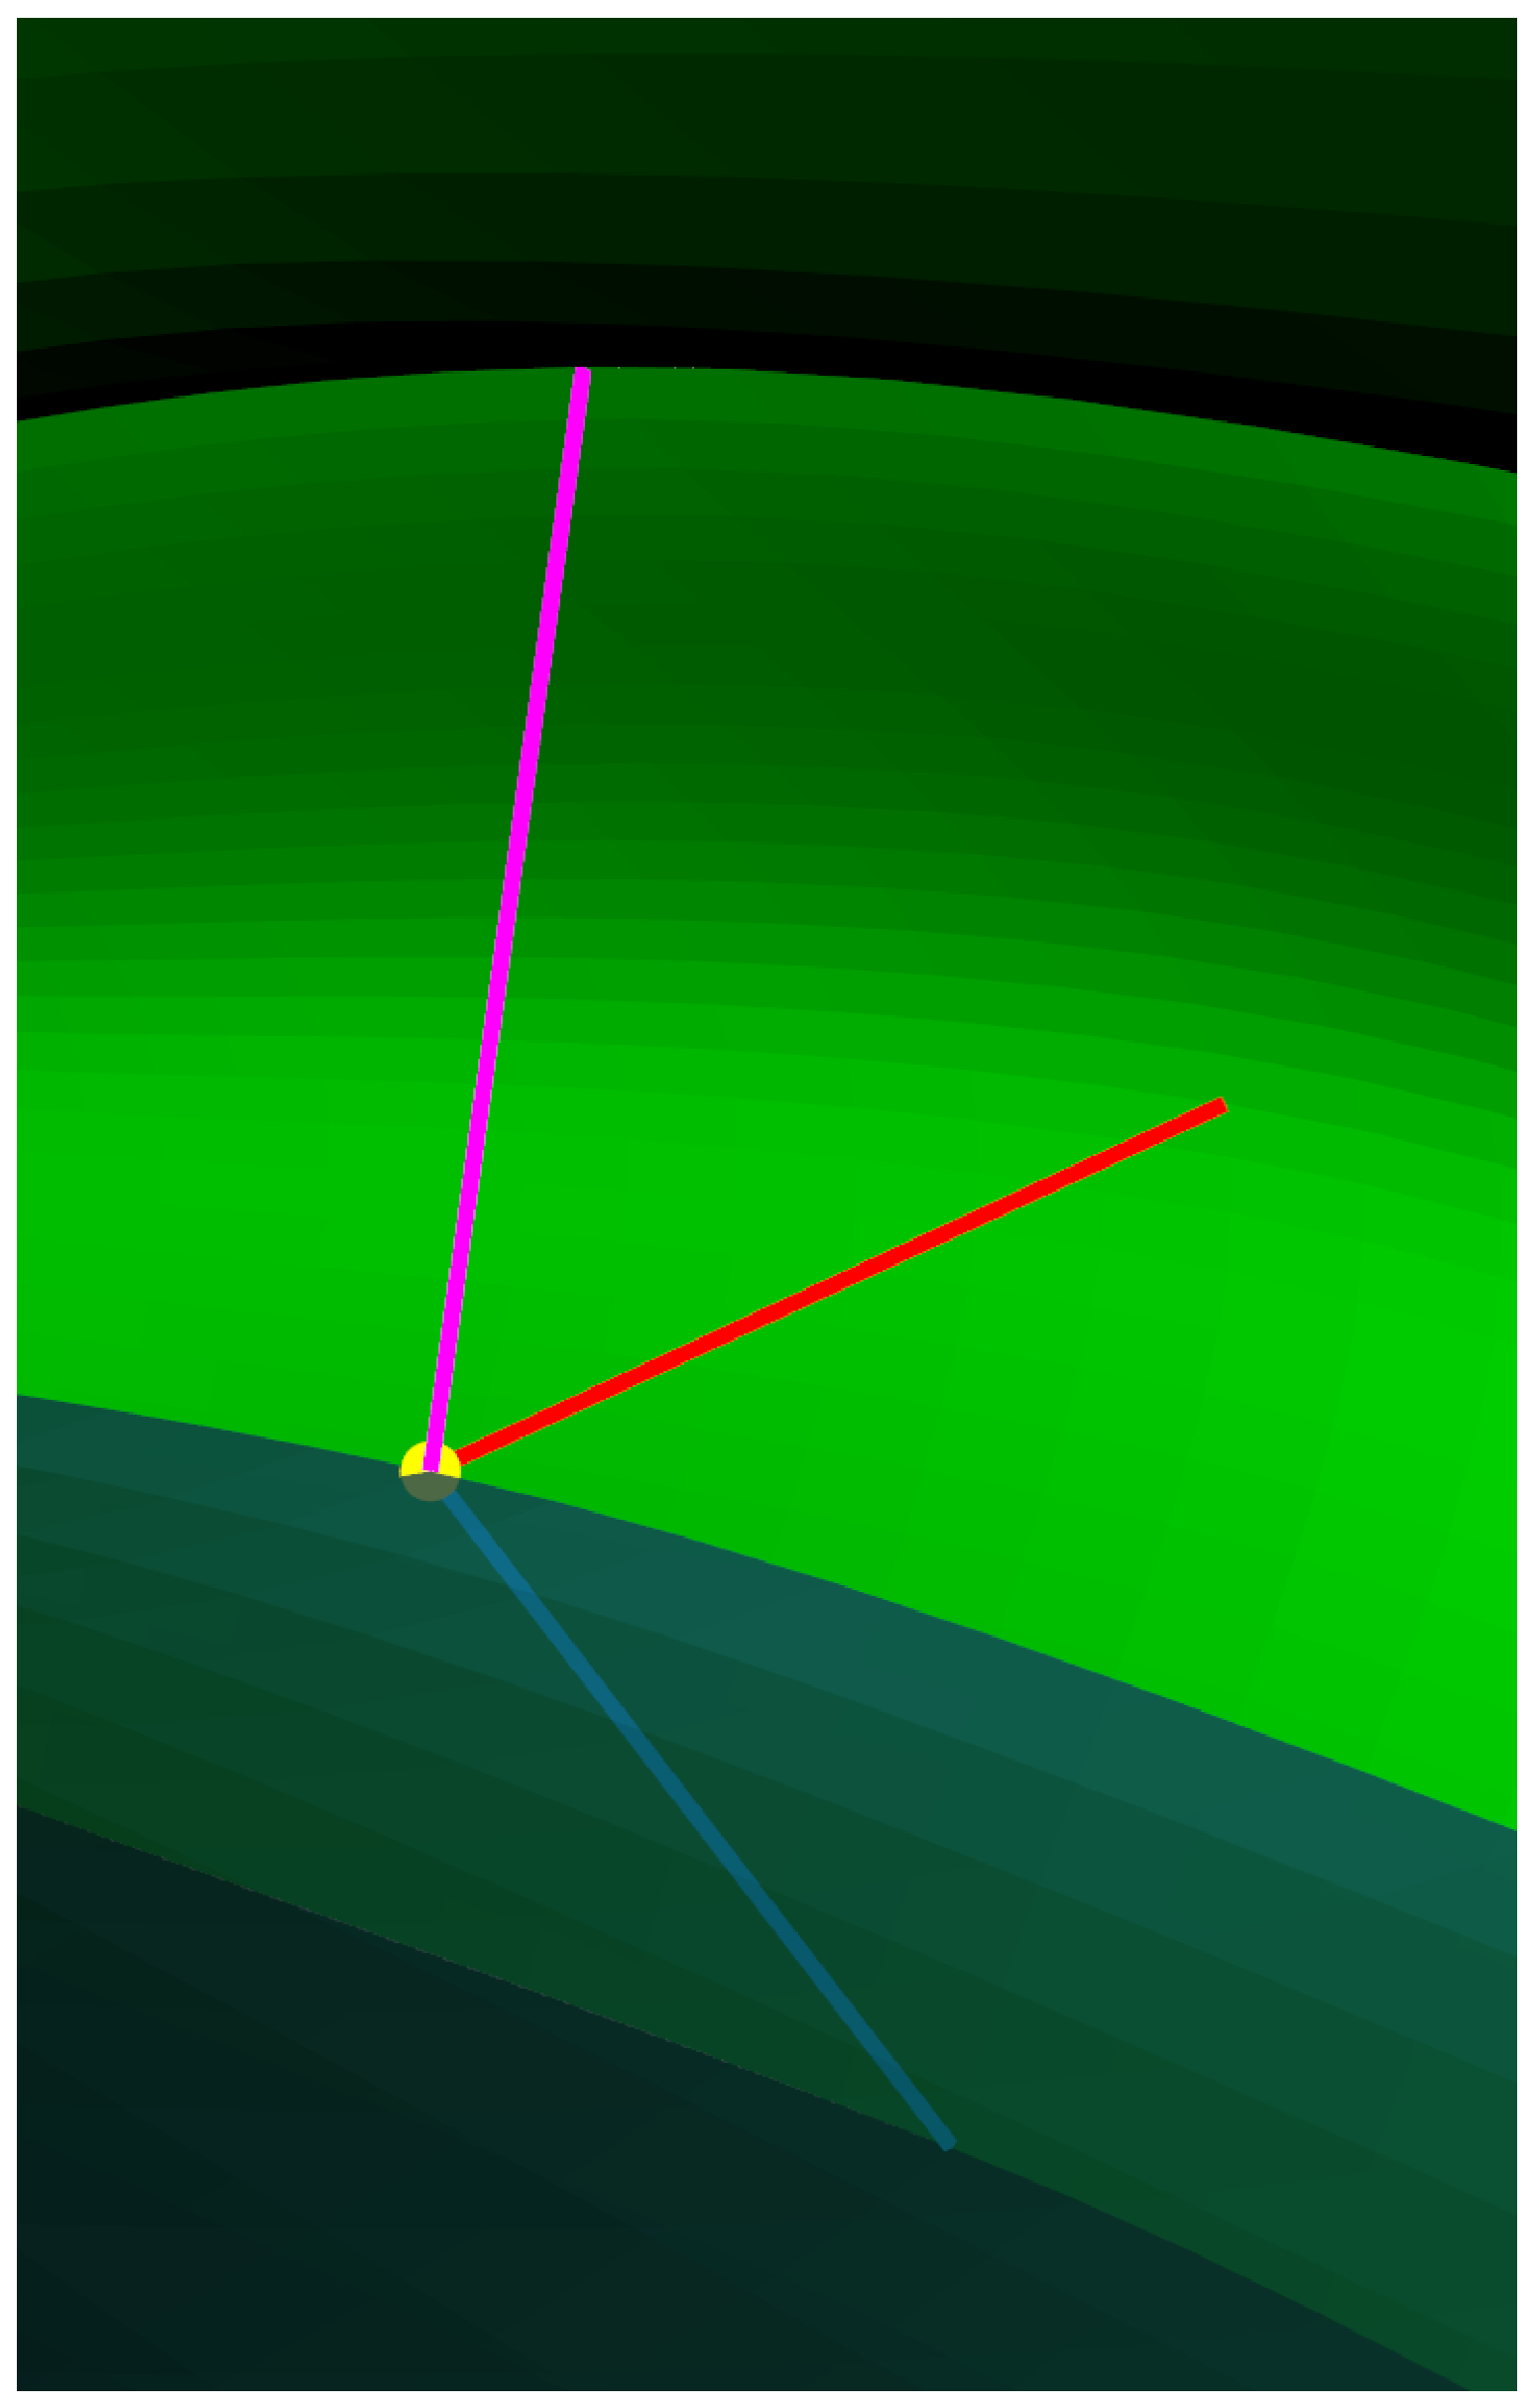
\epsfig{file = s-repatomCloseUp.eps, width = 3.25cm}}
	\subfigure[]{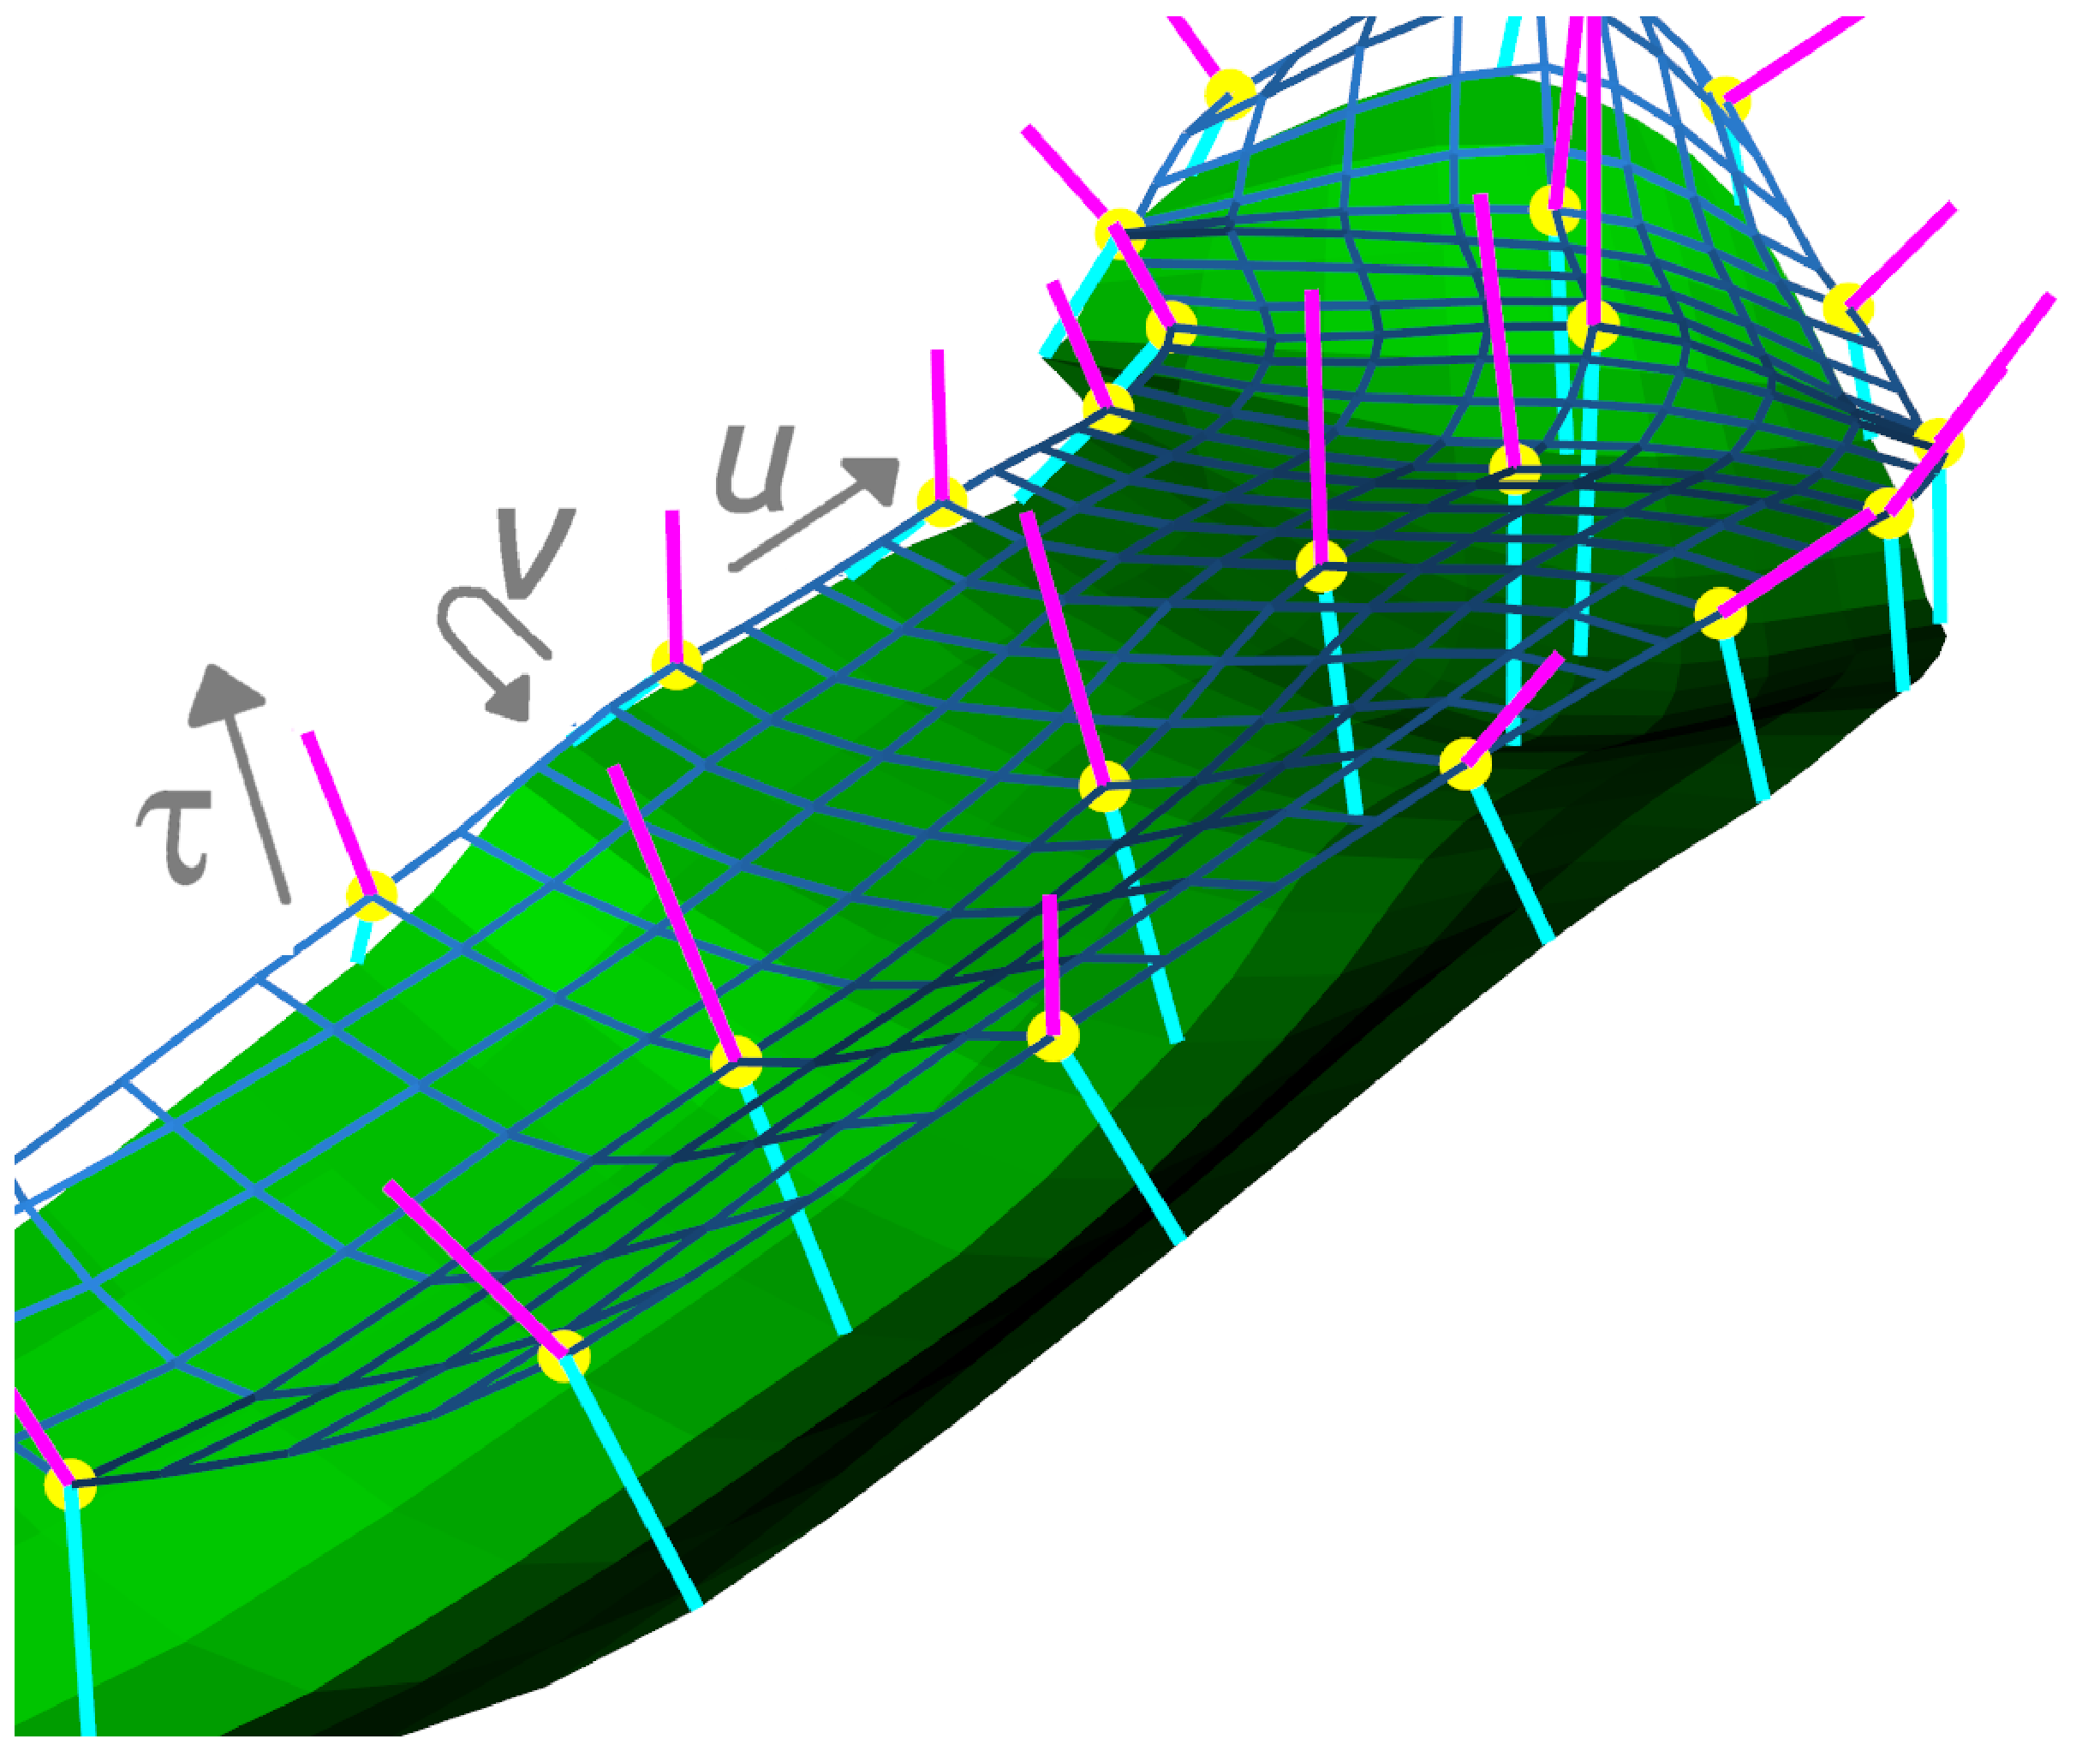
\epsfig{file = s-repFig.eps, width = 6cm}}
	\subfigure[]{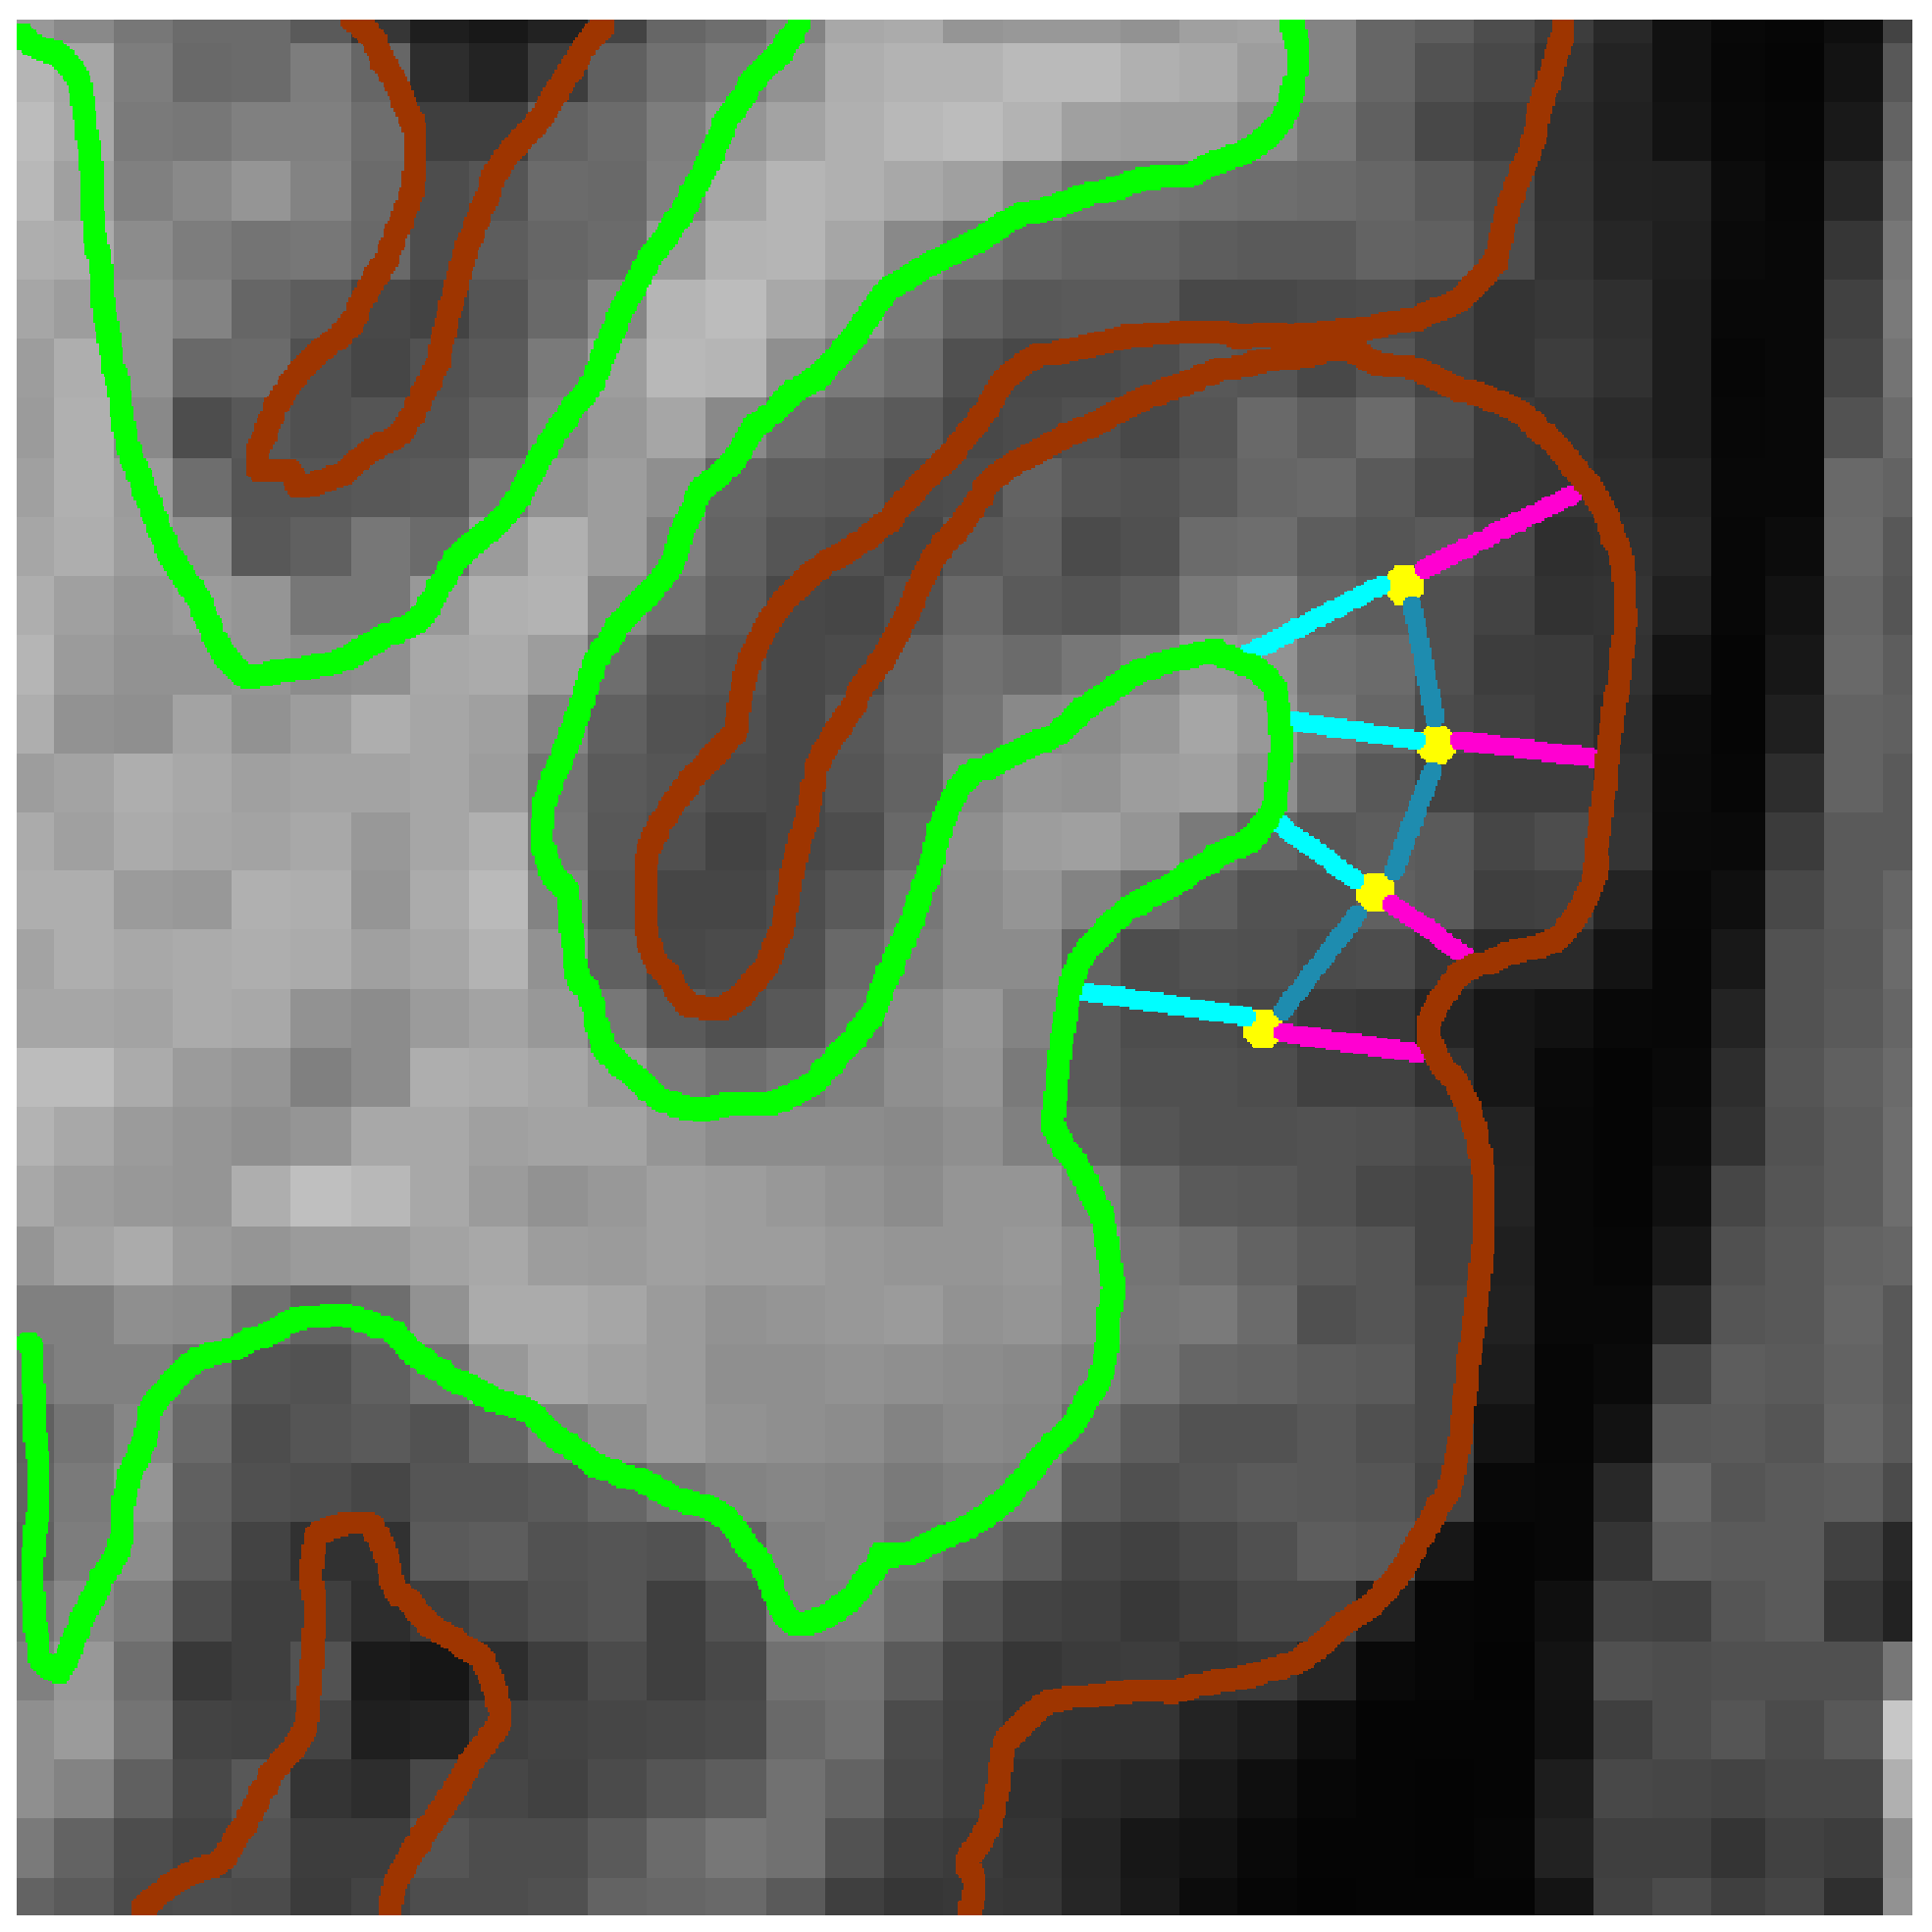
\epsfig{file = lh_BrainFreesurferZoom.eps, width = 5cm}}
 \caption[Atom close up.]{Figure (a) shows a close up of an atom represented as the yellow ball with its corresponding spokes, top (magenta), bottom (cyan), crest (red). 
          The s-rep on figure (b) shows the quasi-medial surface in wireframe representation (blue), with the sampled atoms.
          The MRI image on figure (c) shows a cross-section of the skeletal locus of the cortex and some atoms with the corresponding top and bottom spokes.}
 \label{fig:srepfigCortex}  
\end{figure}

%S-reps are defined as continuous objects using the interpolation mechanisms described in \cite{pizer_nested_2012},
%meaning that every point inside the object has a unique set of coordinates $[u, v, \tau]$. $u$ codes the width, $v$ the length of the medial locus,
%and $\tau$ the thickness of the object.
%$u$ varies from 0 to 1, $v$ wraps around the object with $v < 0.5$ on the ``anterior'' and $v > 0.5$ on the ``posterior'', and $\tau$ 
%from the skeletal locus to the object boundary, as shown in Figure \ref{fig:Srepfig}-b.
%The union of vectors form the object boundary and the union of tails represent the ``skeletal locus''. 
%Notice that s-reps model the continuum space, opening the possibility to include the cellular level and describe the layered structure 
%of the cortex.
Figure \ref{fig:srepfigCortex} shows how an s-rep fits into the cortex. 
%From now on the word s-rep is used to reference the discrete version of the object.

Besides shape description, s-reps have been used successfully to compute shape statistics and mean shapes from a population 
of objects. 
%This is done using CPNS a method analogous to PCA \cite{pizer_nested_2012}.
With this statistical description, it appears to be possible to classify objects by shape frequently more accurately than any other method.
%The majority only use surface information; in contrast, the skeletal structure brings 
%stability to the statistics and increases the correspondence of information across the population of objects.
%S-reps have been used to model internal brain structures such as the hippocampus \cite{pizer_nested_2012}. 
S-reps model single non-branching objects, and tubular objects, as explained in Section \ref{sec:quasiMedial}.
The objects modeled with s-reps until now are simple as most of them have a 
blob-like or elongated shape structure like the the hippocampus \cite{pizer_nested_2012}.

It is demonstrated that s-reps are suited to represent a folded complex structure such as the cortex.
The sheet of the object does not branch and captures the majority of the folds in the cortex. 
Moreover, a statistical analysis of shape variability is done using the s-rep description of the cortex.

The following section explains how to create an s-rep of the cortex from an MRI image.
The procedure uses a spherical representation of the cortex  \cite{fischl_cortical_1999} 
that relates the WM and the GM surfaces to the sphere.
Folding the s-rep into the cortex is done by 
projecting the SS (skeletal sheet) of the s-rep on the sphere and 
using the relationship of the sphere and the cortical surfaces.
%The folding procedure uses a function 
%that minimizes the distance to a set of closest points in the WM and GM surfaces.
%The procedure is done for every atom. It maintains
%the topology and regularity of the quads 
%or quadrangles that form the SS of the s-rep (quad definition in Equation \ref{equ:Quad}).
The following section explains in detail the procedure to create an s-rep of the cortex.
With the skeletal figure inside the cortex, 
top and bottom spokes point towards the GM and WM surfaces respectively.
The interpolation mechanisms of the s-rep allows reconstructing the GM surface and the WM surface.
Section \ref{sec:Evaluation} evaluates the quality of the interpolated surfaces.
Finally, a population of cortex s-reps is generated, and a statistical analysis is made in Section \ref{sec:Statistics} using CPNS (Composite Principal Nested Spheres, which is  
described in Appendix \ref{sec:apendixCPNS}).

\section{Acknowledging the true shape of the cortex}
\label{sec:s-repFittingCortex}


\begin{figure*} 
 \centering 
	\epsfig{file = DiagramProy.eps, width = 15cm}
 \caption[Flow diagram of s-rep projection and cortex folding.]{(a) Inflation of the cortex by \textit{Freesurfer} and rotation of the sphere to the north using the points in the corpus callosum. 
          (b) Transformation of a base s-rep into a circle.
          (c) Transformation of the circle into a sphere. 
          (d) Fitting the s-rep to \textit{Freesurfer's} data on the sphere.
          (e) Folding the SS of the s-rep inside the the cortex and determine the widths of the slab. 
          }
 \label{fig:proyProcedure}  
\end{figure*}

The cortex is a highly folded sheet. It has thickness that varies through the cortical regions. 
Unfortunately, the cortex is often represented using surfaces and is difficult to 
represent interior  features.
To acknowledge its true shape which is similar to a folded pancake, 
a procedure to create an s-rep of the cortex is proposed. 
As shown in Figure \ref{fig:proyProcedure}, the procedure has five steps:

\begin{enumerate}[(a)]
 \item A mapping of the cortex on a sphere is done using the method from \cite{fischl_cortical_1999}. 
       The sphere is rotated to the north using the corpus callosum.
 \item A regular grid or the SS of a base s-rep is transformed into a 'circular log-grid'.
 \item The 'circular log-grid' is transformed into a sphere (with a spherical cap oppening in the north pole).
 \item The SS on the sphere is fitted to the mapping of the cortex on the sphere.
 \item The SS is folded back into the shape of the cortex. During the folding procedure, the widths of the slab or the thickness of the s-rep is determined.        
\end{enumerate}

The following sections explain the details of each step and shows how to create an s-rep 
of the cortex.


\subsection{Spherical representation of the cortex by \textit{Freesurfer} and rotation}
\label{sec:Materials}

The materials used in this study are 8 
MRI scans acquired at ``CERMEP - Imagerie du vivant'' 
%********************* 
on a Siemens 
Sonata system with a 1.5 T magnet, with gradients of 40 mT/m and an 8-channel head coil. 
The overall protocol includes anatomical acquisitions, spectroscopy and diffusion.

In this study, only T1-weighted anatomical images are considered. The 8 datasets were obtained by
the acquisition of millimetric sagittal slices from a 3D T1-weighted MPR sequence (repetition time (TR) = 1880 ms, echo time (TE)
Ms = 4).
The total acquisition time of each of these anatomical images was done in 18 minutes.

All the datasets were segmented using \textit{Freesurfer}.
%and the inflation and flattening procedure from \cite{fischl_cortical_1999}.
The method proposed by \cite{fischl_cortical_1999} 
creates a spherical representation of the cortex. It removes the folds from the surface using an energy functional 
with a distance term for unfolded or positive regions. 
An unfolded region is recognized by calculating the normal direction and the ordered cross-product
of the triangle legs for every face in the surface tessellation. If the resulting vector 
is anti-parallel to the normal direction, a negative area is assigned. 
The folds from the surface are eliminated when the area is constrained to be
positive everywhere.
After the inflation procedure, the cortical surface has spherical topology. 
A mapping of the cortex is made onto a sphere providing 
a $1-1$ relationship for every point on the cortical surface and spherical mapping.
%The spherical mapping is the key to construct the s-rep of the cortex. 

The procedure to build the s-rep of the cortex uses a modified stereographic projection.
The stereographic projection \cite{snyder_map_1987} was probably known to the Egyptians in its polar form, 
but Hipparchus (2nd Century B.C) was apparently the first Greek to use it, so he is considered its inventor. 
Ptolemy referred to it as ``Planisphaerum'', the name stereographic was given by Fran\c{c}ois d'Aiguillon in 1613.
The stereographic projection enables a mapping of the points on a plane
to the sphere and it has two properties that should be treated carefully:
%is conformal (preserves angles), azimuthal (all points are proportionally correct distances from the center point),
the scale increases away from the center of the projection,
and the point opposite to the center of the projection cannot be plotted (north pole).

The first step to do a stereographic projection is to choose the north pole. 
The north pole of the sphere cannot be mapped by the stereographic projection because it
maps to infinity. For this reason, the representation must have a spherical cap opening in the north pole.

The corpus callosum is a brain structure located 
beneath the cortex. It facilitates inter-hemispheric communication with a bundle of 200-250 million fibers for this task.
Figure \ref{fig:Corpuscallosum} displays the corpus callosum. 
This brain structure is used to find the north pole.
The points in the corpus callosum are used in a fitting procedure that minimizes the geodesic distance from each point to a circle. 
The center of the best fitting circle is chosen to be the north pole.
%The point opposite to the north pole is the center of projection.

\begin{figure} 
 \centering 
 \subfigure[The internal part of the left hemisphere of the cortex. 
            The corpus callosum is shown in the figure.
            The points that compose the corpus callosum are used in the minimization procedure.]{\epsfig{file = corpuscallosum.eps, width = 7.25cm}}
 \subfigure[Spherical representation of the left hemisphere. 
            The best fitting circle is shown in cyan and the projected points  
            on top of the circle in magenta. The center of the circle is aligned with the north pole.]{\epsfig{file = sphereRotationNorth.eps, width = 7.25cm}}
 \caption[Inflation procedure, mapping the cortex on a sphere.]{The inflation procedure maps the cortical surface onto a sphere. 
          The best fitting circle is found using the points of the corpus callosum.}
 \label{fig:Corpuscallosum}  
\end{figure}

To find the best circle for a set of points in a sphere, a method similar to \cite{jung_analysis_2012} is used.
A circle on the sphere $S^2$ is defined by a vector $v_1$ and a distance $r_1 \in (0, \pi/2]$ as in equation \ref{equ:circle0},
where $\rho_d$ is the geodesic distance function.

\begin{equation}  
	C(v_1, r_1) = \{x \in S^2 : \rho_d(v_1, x) = r_1\}.
  \label{equ:circle0}
\end{equation}
The best fitting circle is found with a least squares minimization
that uses the geodesic distance as follows:
let $CC = \{x_i: i \in N\} \in S^2$ be the points of the corpus callosum on the sphere. We first define the residual $\varepsilon$ of $x_i$ from a circle
$C( v_1 , r_1 )$ of $S^2$ as the signed length of the minimal geodesic that joins $x_i$ to $C$. Then 
$\varepsilon = \rho_d( v_1 , x ) - r_1$. The sign of $\varepsilon$ is negative if $x_i$ is in the interior of $C$, and is positive if $x_i$ is in the exterior.
The best fitting circle $\hat{C} \equiv C( \hat{v}_1 , \hat{r}_1 )$ 
is found by minimizing the sum of squares of residuals of the data points to $C$. 
In other words $v_1$ and $r_1$ minimize Equation \ref{equ:optimalcircle}.

\begin{equation}  
  \hat{C} = \operatorname*{Arg\,min}_{v_1, r_1} \sum_{i=1}^{n} \varepsilon_i ( v_1 , r_1 )^2 = \operatorname*{Arg\,min}_{v_1, r_1} \sum_{i=1}^{n}\{\rho_d(x_i, v_1) - r_1 \}^2
  \label{equ:optimalcircle}
\end{equation}

Once the center of the circle is found, 
a rotation is done to align its center to the north pole. 
%A second rotation is performed to align it with the x axis. 
%This is done by finding the average point on the circle for the projected data, calculating the tangent at this point,
%and computing the opening angle with the x axis.
Figure \ref{fig:Corpuscallosum} shows the corpus callosum and a spherical representation 
of the cortex with the best fitting circle. 

The following section explains how to modify the s-rep 
to produce the best possible mapping on the sphere. 
The projection to the sphere is explained in Section \ref{sec:StereographicProjection}.

\subsection{Transforming the s-rep into a circular log grid}

An s-rep is built using a grid of sampled points where
each intersection is a hub or atom of the s-rep. 
An atom is defined as a sampled point on the SS or quasi-medial surface of the object as shown in Figure \ref{fig:srepfigCortex}-a.

To generate the s-rep of the cortex, the structured collection of atoms (the grid) is mapped on a sphere.
This mapping is equivalent to the mapmakers problem, \textit{i.e.}, to map two surfaces with
different Gaussian curvatures. This was shown to be impossible by Gauss in 1828.
To lower the distortion effects of the projection and allow the construction of the s-rep, 
the grid of the s-rep is modified.
This is done to improve the sampling of the hubs on the sphere while preserving the grid topology.

Relating the points from the plane to the sphere is the key to produce the s-rep of the cortex. 
Each projected hub can be related to the spherical representation of the cortex provided by \textit{Freesurfer}.
%(an automated tool for brain's cortical surface reconstruction using structural MRI data).

\begin{figure}[h!]
 \centering 
 \subfigure[Regular grid]{\epsfig{file = regularGrid.eps, width = 4.5cm}}
 \subfigure[Log grid]{\epsfig{file = logGrid.eps, width = 4.5cm}}
 \subfigure[Circular log grid]{\epsfig{file = logGridCircular.eps, width = 4.5cm}}
 \caption[Resampling of the s-rep.]{An s-rep is represented with a grid of points. If the regular grid is projected on the sphere
          a distortion effect is produced by the stereographic projection. In order to lower the distortion effects, the grid is resampled
          using a log function. The transformation into a circle is done to match the s-rep to the best-fitting circle of the corpuscallosum.}
 \label{fig:gridTransformation}  
\end{figure}

An s-rep is represented by a regular grid on a plane.
Mapping a regular grid on the sphere 
causes a distortion since 
the majority of the hubs will map towards the north pole (first property of the stereographic projection).
To produce the best s-rep of the cortex and capture accurately the geometry of the folds,
the hubs should be spaced evenly on the sphere. 

To attain a regular spacing of the hubs, a log function is used to resample the position of the hubs in the grid. 
Figure \ref{fig:gridTransformation} shows how the log function maps more points towards the center of projection.

\begin{equation}
  S(x) =  \left\{
		  \begin{array}{lr}
			  Min + x*(\frac{Max - Min}{N/2}), & x < \frac{N}{2} \\
			  Min + (N-x)*(\frac{Max - Min}{N/2}), & otherwise
		  \end{array}
  \right.  
  \label{equ:step}
\end{equation}

\begin{equation} 
 L(S(x)) = \left\{\begin{array}{lr}
			  \frac{log(S(x))}{log(Min)}, & x < \frac{N}{2} \\
			  -\frac{log(S(x))}{log(Min)}, & otherwise
		  \end{array}
		  \right.
  \label{equ:logscale}
\end{equation}

Equations \ref{equ:step} and \ref{equ:logscale} show how to transform the regular grid.
Each hub $(x,y) \in [0, N-1]$ is distributed regularly with $S(x) \in [Min, Max]$
where $N$ is the number of points for one side of the grid,
$Min \in (0, Max)$, and $Max$ is always set to 1.
$L(S(x)) \in [-1, 1]$ moves the points towards the center 
of projection (south pole). Having an increased number of 
points near the center reduces the distortion effects 
produced by the stereographic projection.

Finally, to further improve the projection of the grid on the sphere, 
the grid is transformed
into a circle as described in \cite{nowell_philip_math}.
By projecting the circle on the sphere, the spherical cap opening
required by the stereographic projections is naturally found.
Equation \ref{equ:squaretocircle} shows how the transformation is done. 
Notice that the points over the axis do not change, points in the corners get normalized and all others are 
transformed accordingly, as shown in Figure \ref{fig:gridTransformation}.
%for an example on the effect of 
%different grid types on the final cortex representation, see Figure \ref{fig:BestCircle}.

\begin{equation}  
	\begin{array}{lcr}
		x' & = & x \sqrt{1 - \frac{1 - y^2}{2}} \\
		y' & = & y \sqrt{1 - \frac{1 - x^2}{2}} 
	\end{array}  
  \label{equ:squaretocircle}
\end{equation}

%\begin{figure} 
%\vspace{-0.2cm}
% \centering 
% \subfigure[Square log grid]{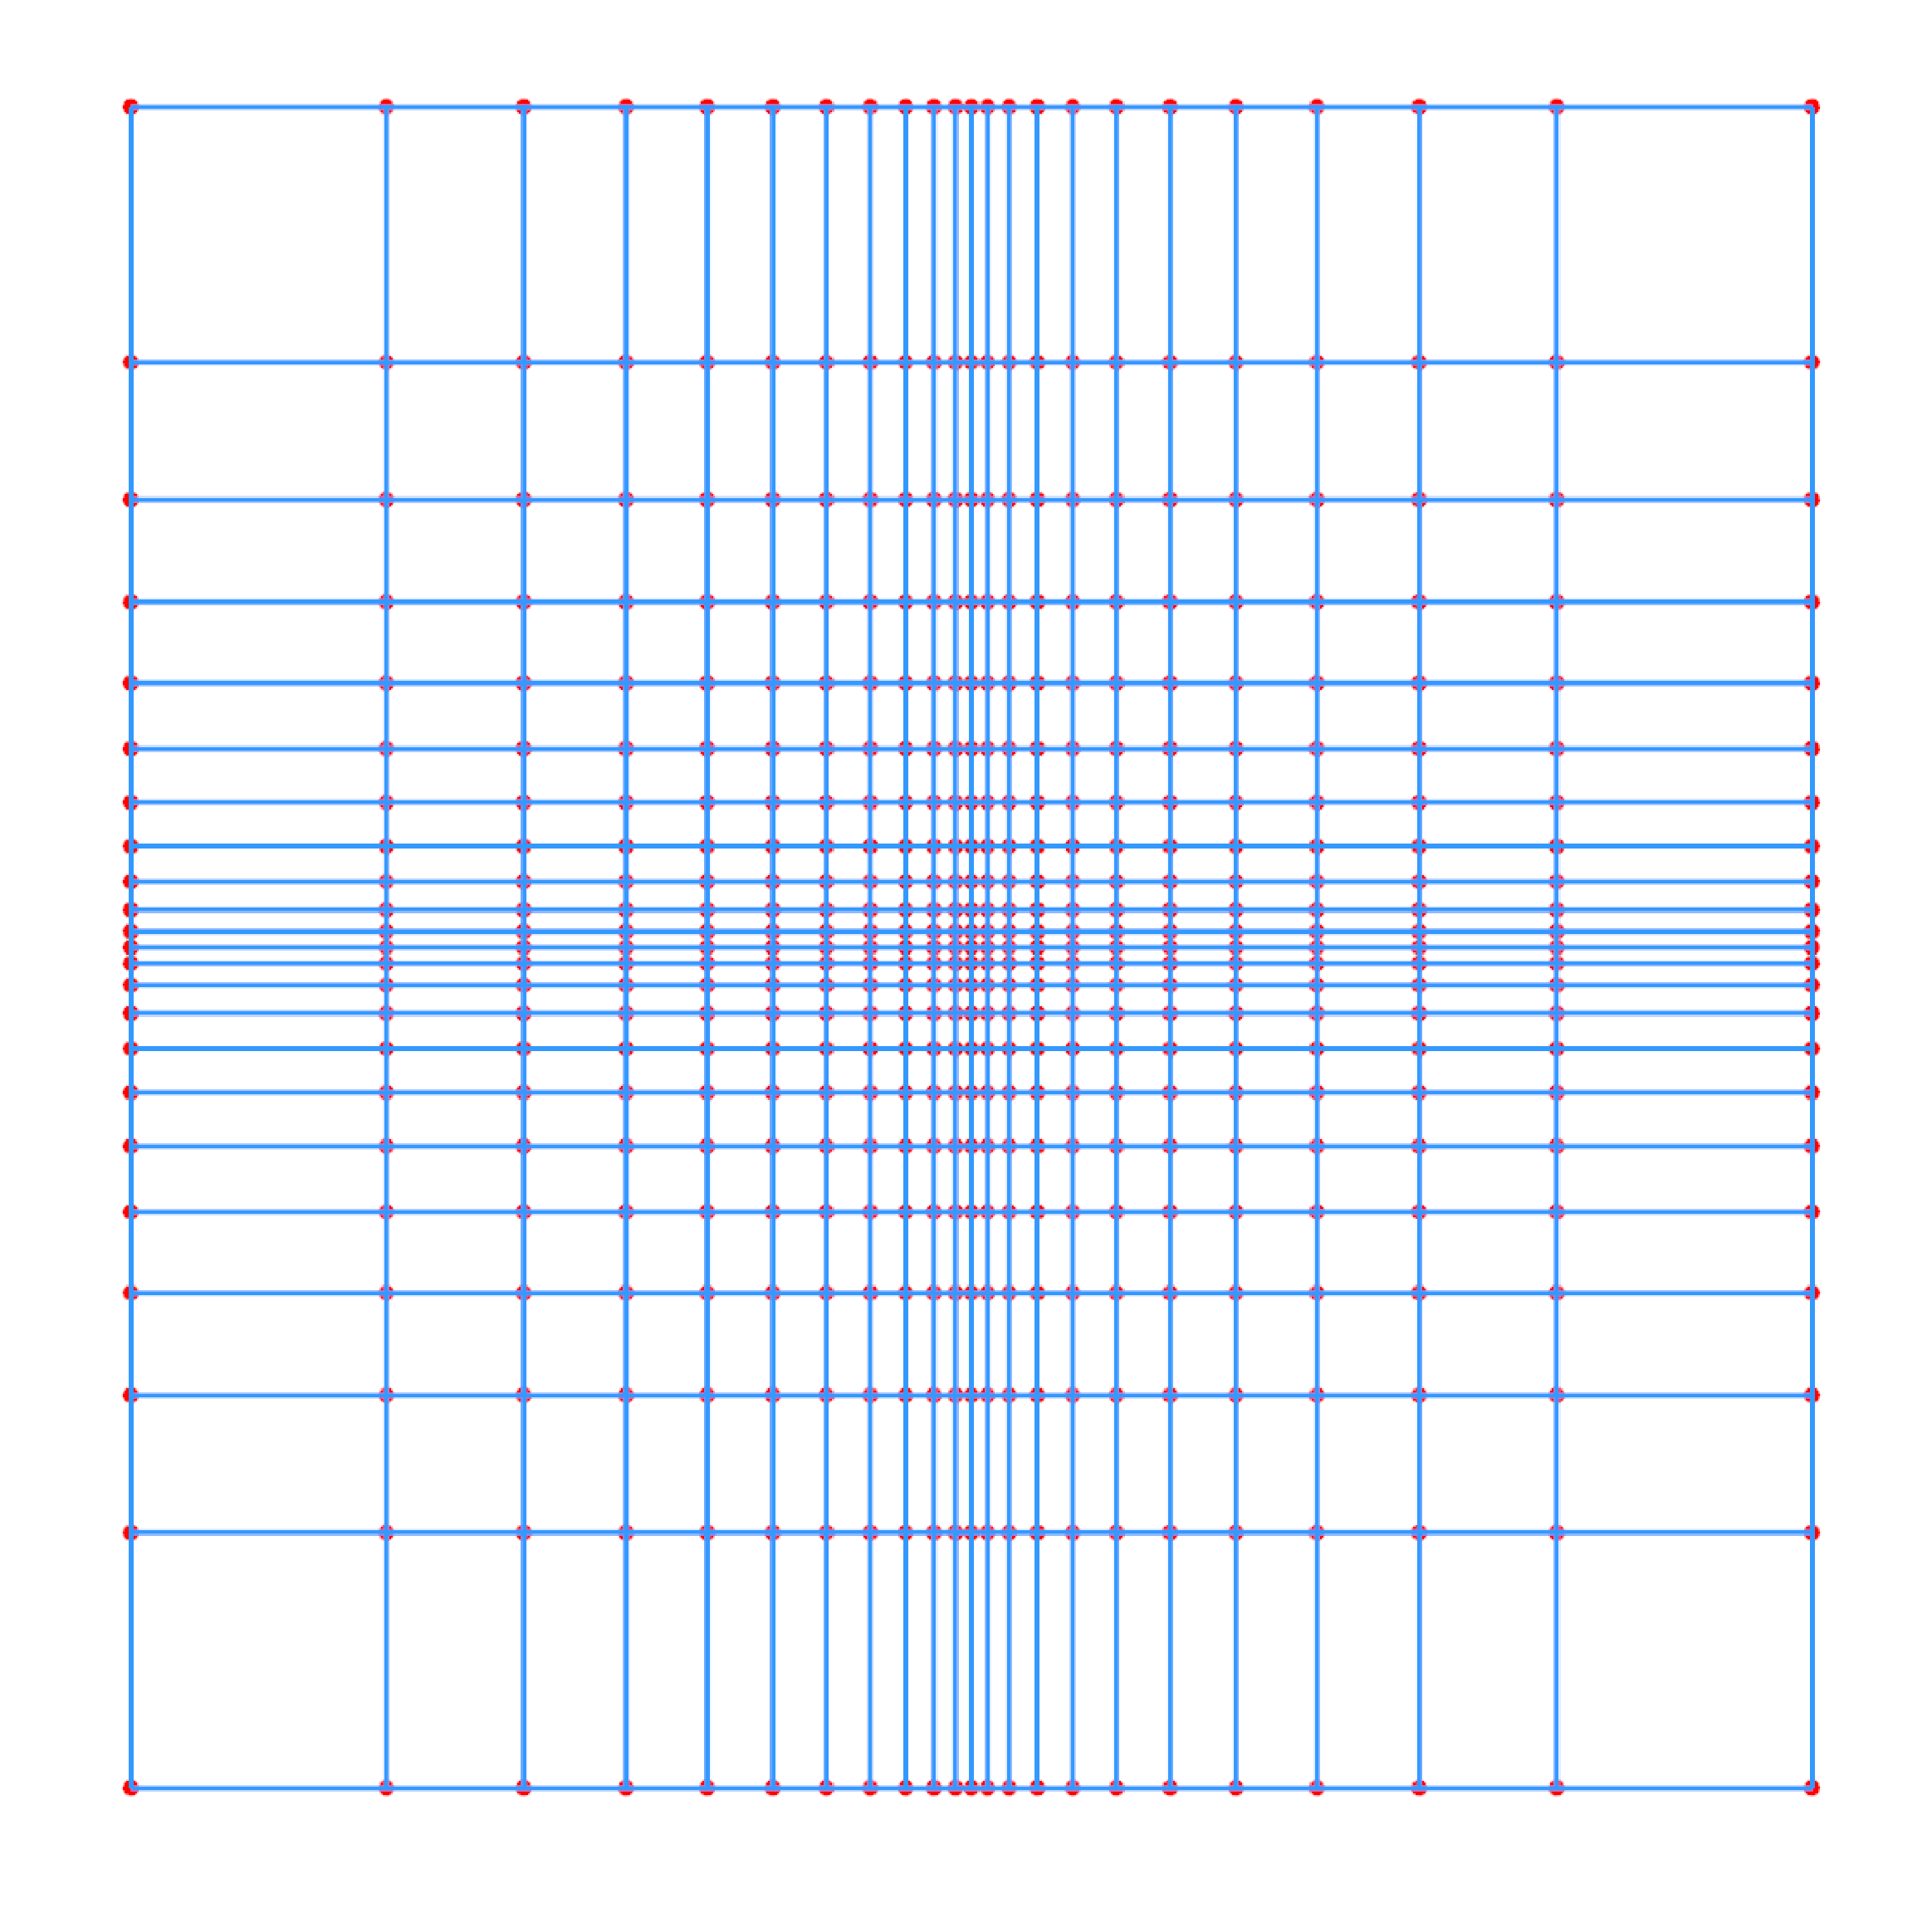
\epsfig{file = square_s-rep.eps, width = 3cm}}
% \subfigure[Circular log grid]{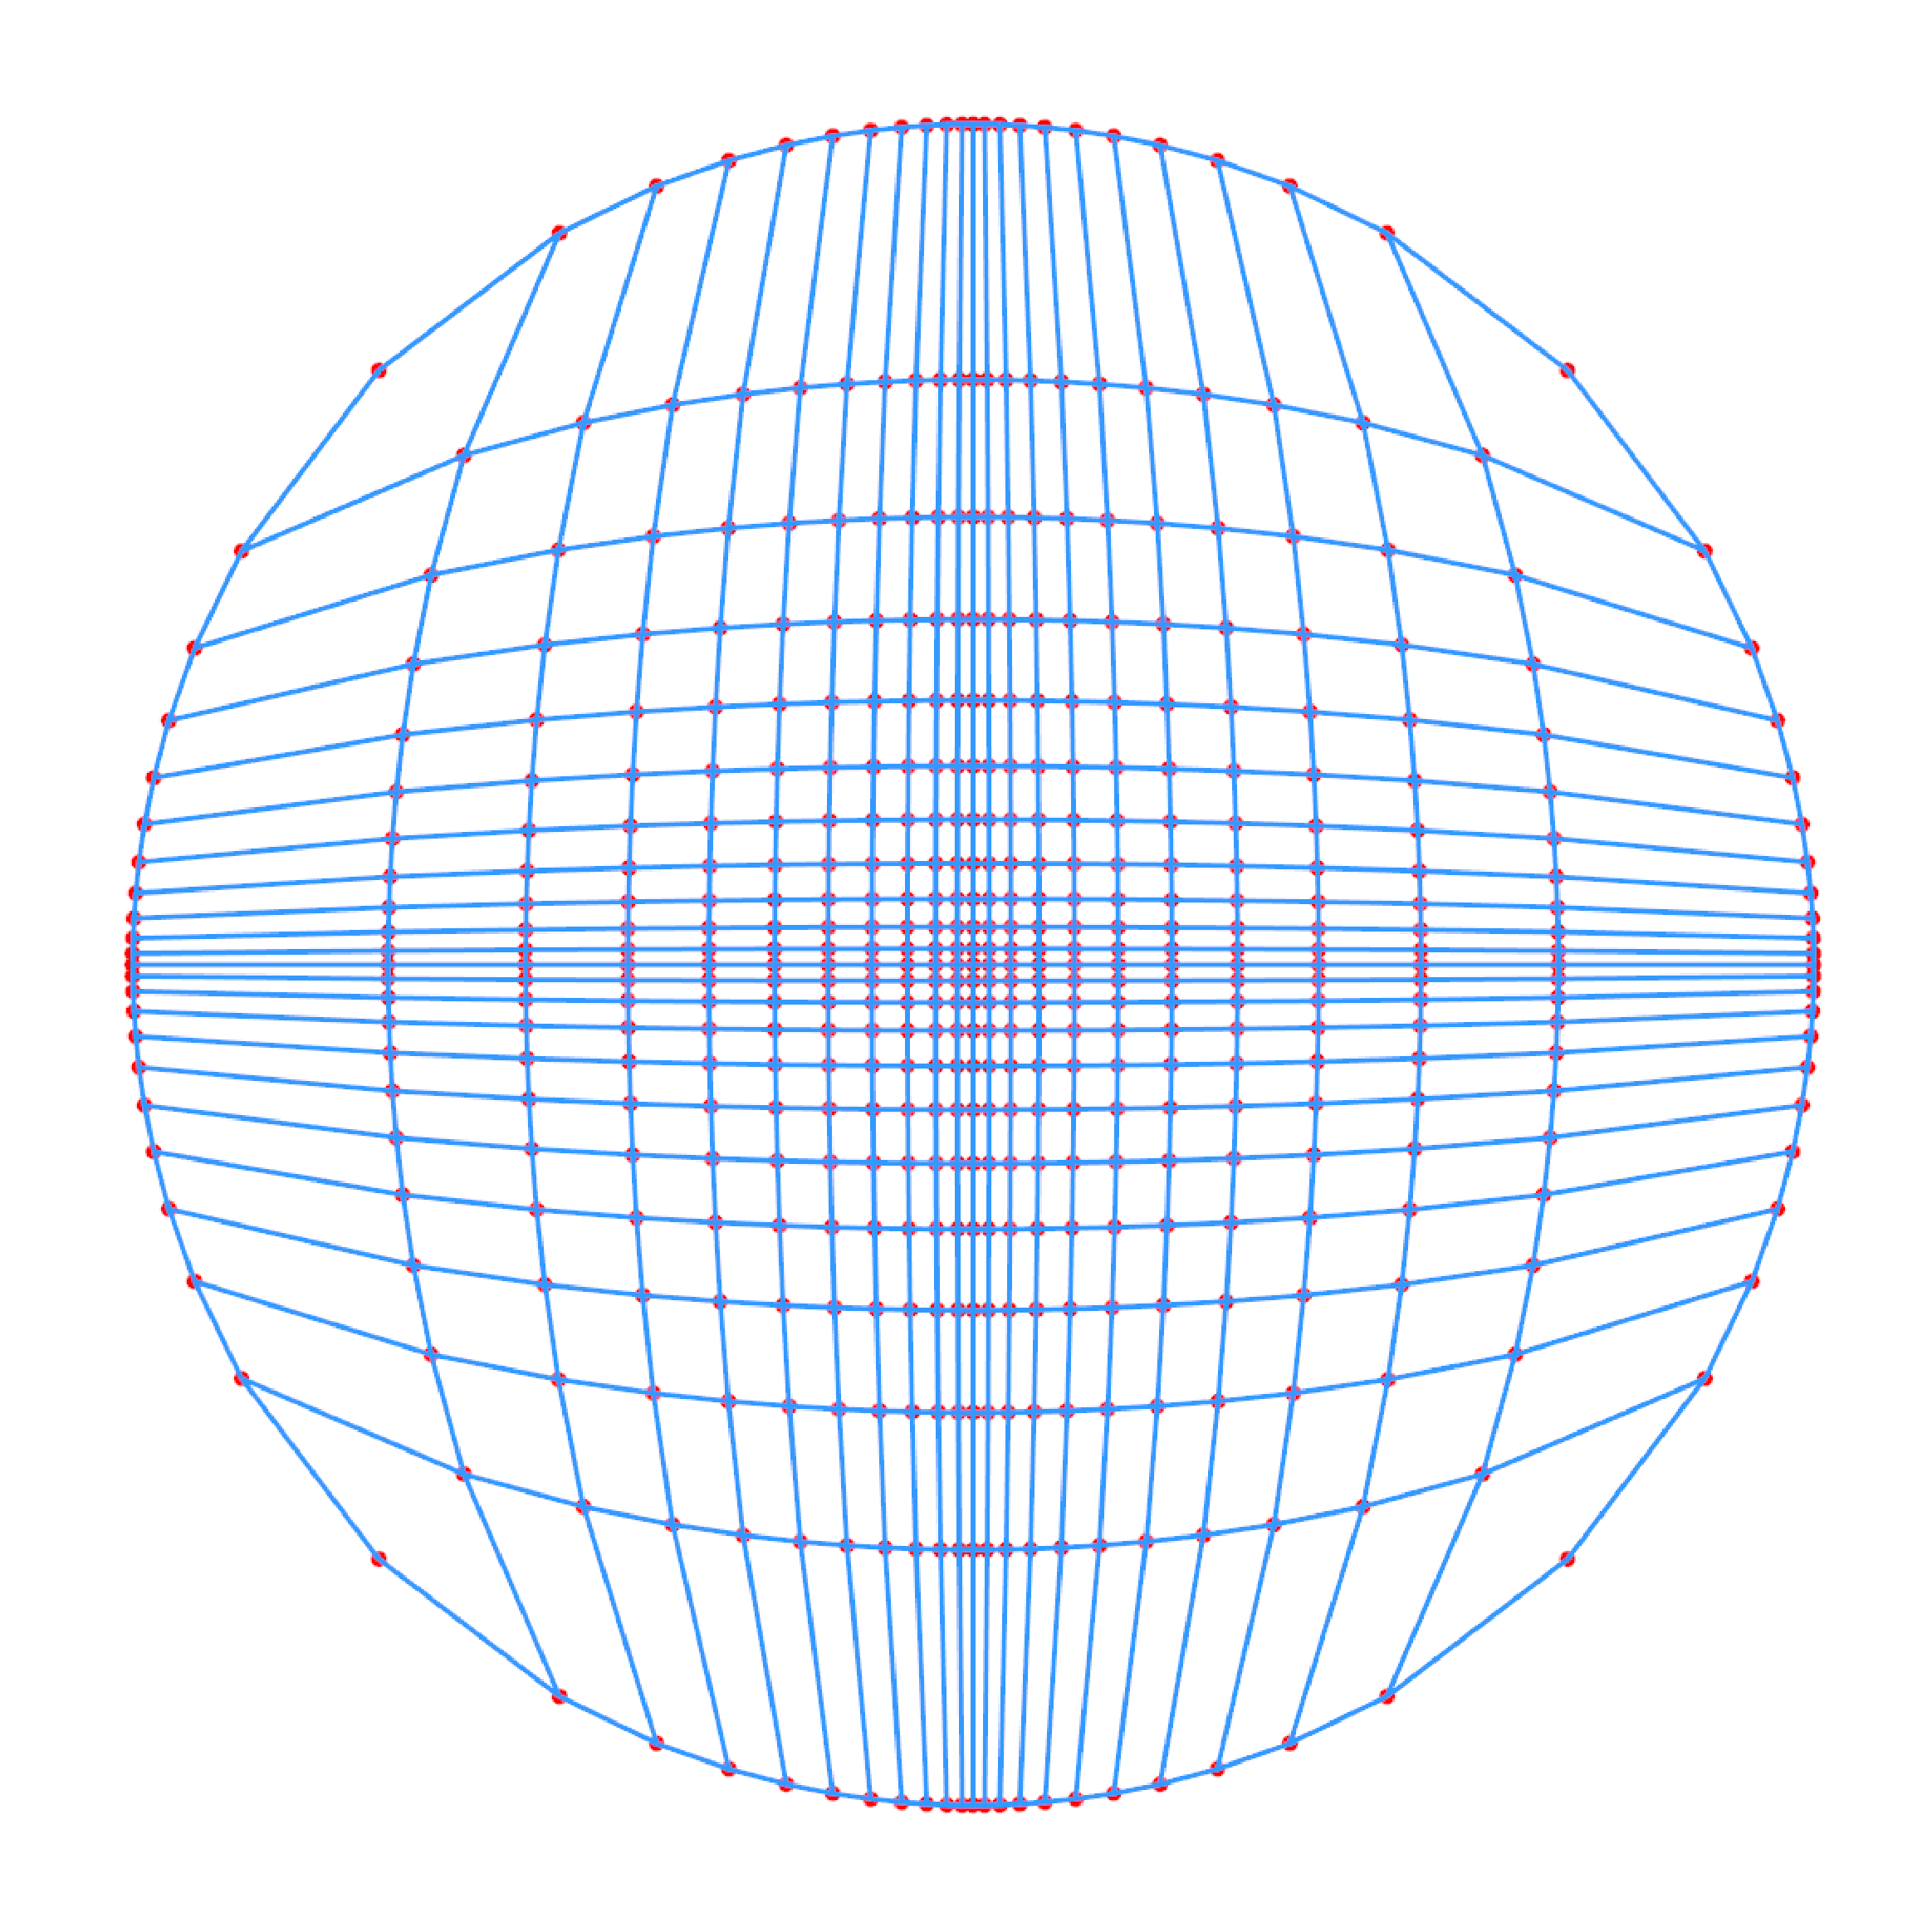
\epsfig{file = circle_s-rep.eps, width = 3cm}}
% \caption{A square grid transformed into a circle on the plane.}
% \label{fig:GridTypes} 
% \vspace{-0.1cm}
%\end{figure}

The following section explains how to project the transformed grid to the sphere.
Figure \ref{fig:SphereSamplingSphere} shows the results of mapping a regular-grid and log-grid on the sphere. 

\subsection{S-rep projection from the plane to the sphere}
\label{sec:StereographicProjection}

Once the ``circular log grid'' is created, the projection 
finds the corresponding positions on the sphere. 
Equation \ref{equ:stereoprojection} shows how the projection is done where $X = L(S(x'))$ and $Y = L(S(y'))$.

\begin{equation}  
	\begin{array}{lcc}
	    xs & = & 2X/(1 + X^2 + Y^2) \\
	    ys & = & 2Y/(1 + X^2 + Y^2) \\
	    zs & = & (-1 + X^2 + Y^2)/(1 + X^2 + Y^2)
	\end{array}
  \label{equ:stereoprojection}
\end{equation}

\begin{figure}[h!]
 \centering 
 \subfigure[Regular grid]{\epsfig{file = regularGridNorthPole.eps, width = 3.5cm}
			   \epsfig{file = regularGridSouthPole.eps, width = 3.5cm}}
 \subfigure[Log grid]{\epsfig{file = logGridNorthPole.eps, width = 3.5cm} 
		       \epsfig{file = logGridSouthPole.eps, width = 3.5cm}}
 \subfigure[Circular log grid]{\epsfig{file = circularLogGridNorthPole.eps, width = 3.5cm} 
		       \epsfig{file = circularLogGridSouthPole.eps, width = 3.5cm}}
		      
 \caption[Sphere's north and south pole sampling.]{The north (left) and south (right) poles are sampled using a regular,  a log grid and a circular log grid. 
						     The log grid sampling maps more points towards the south pole, and the circular grid 
						     produces the spherical cap opening in the representation.}
 \label{fig:SphereSamplingSphere}  
\end{figure}

Figure \ref{fig:SphereSamplingSphere} shows how the points from the regular grid and the log grid map 
on a sphere. The latter has better hub distribution on the sphere and produces a better s-rep of the cortex. 

Once the hub positions are sampled on the sphere, a fitting procedure to the spherical data provided by \textit{Freesurfer} is done.

\subsection{Fitting the s-rep to \textit{Freesurfer's} data}

At this point there are two spherical representations. 
The first one corresponds to a cortex;
the second one corresponds to the s-rep's SS.

To fit the s-rep to the spherical representation of the cortex,
each hub position is used as input to search for a set of closest points on 
the spherical representation of the cortex.
The searching procedure uses as standard closest neighborhood search algorithm 
with kd-trees. The kd-tree quickly locates the closest points on the sphere from \textit{Freesurfer}.

The folding procedure in the following section uses the points found
and their relationship to the GM and WM surfaces in order to fold the s-rep into the cortex.

\subsection{Folding the s-rep: from the sphere to the cortex}

%\begin{figure} 
% \centering 
% \subfigure[Circular grid]{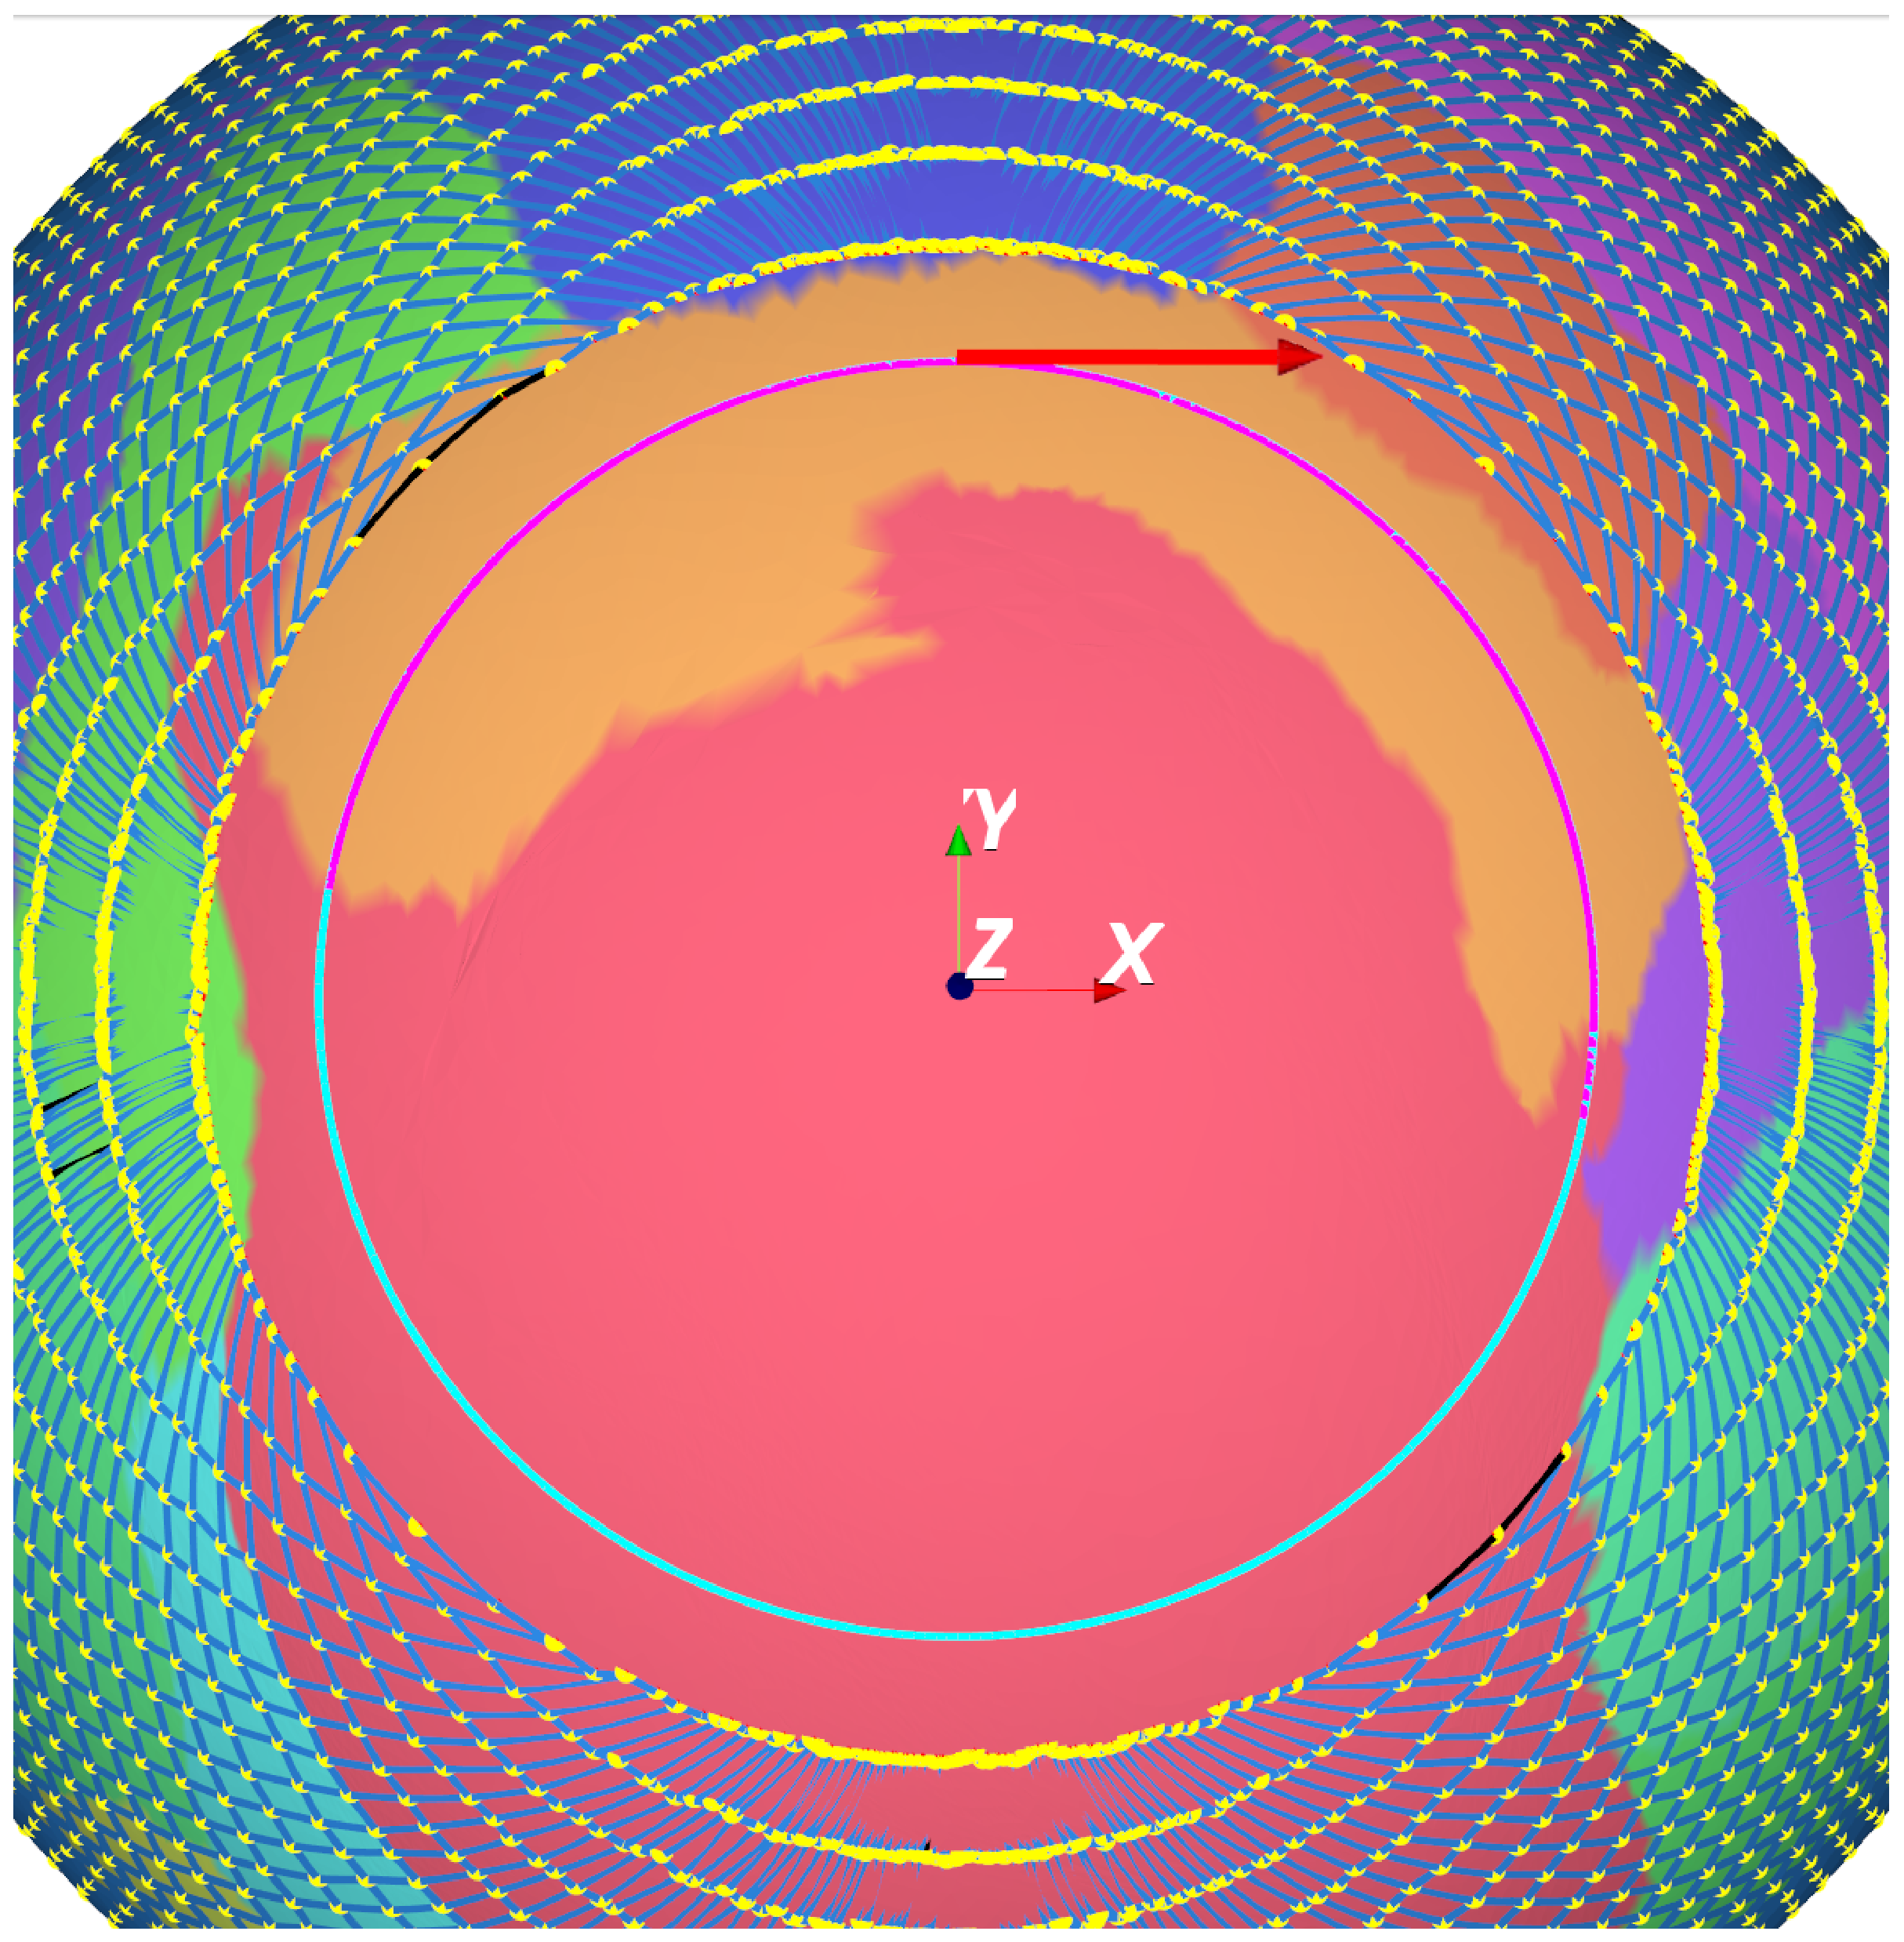
\epsfig{file = fittedSrepSphereCircularGrid.eps, width = 2.75cm}
%			   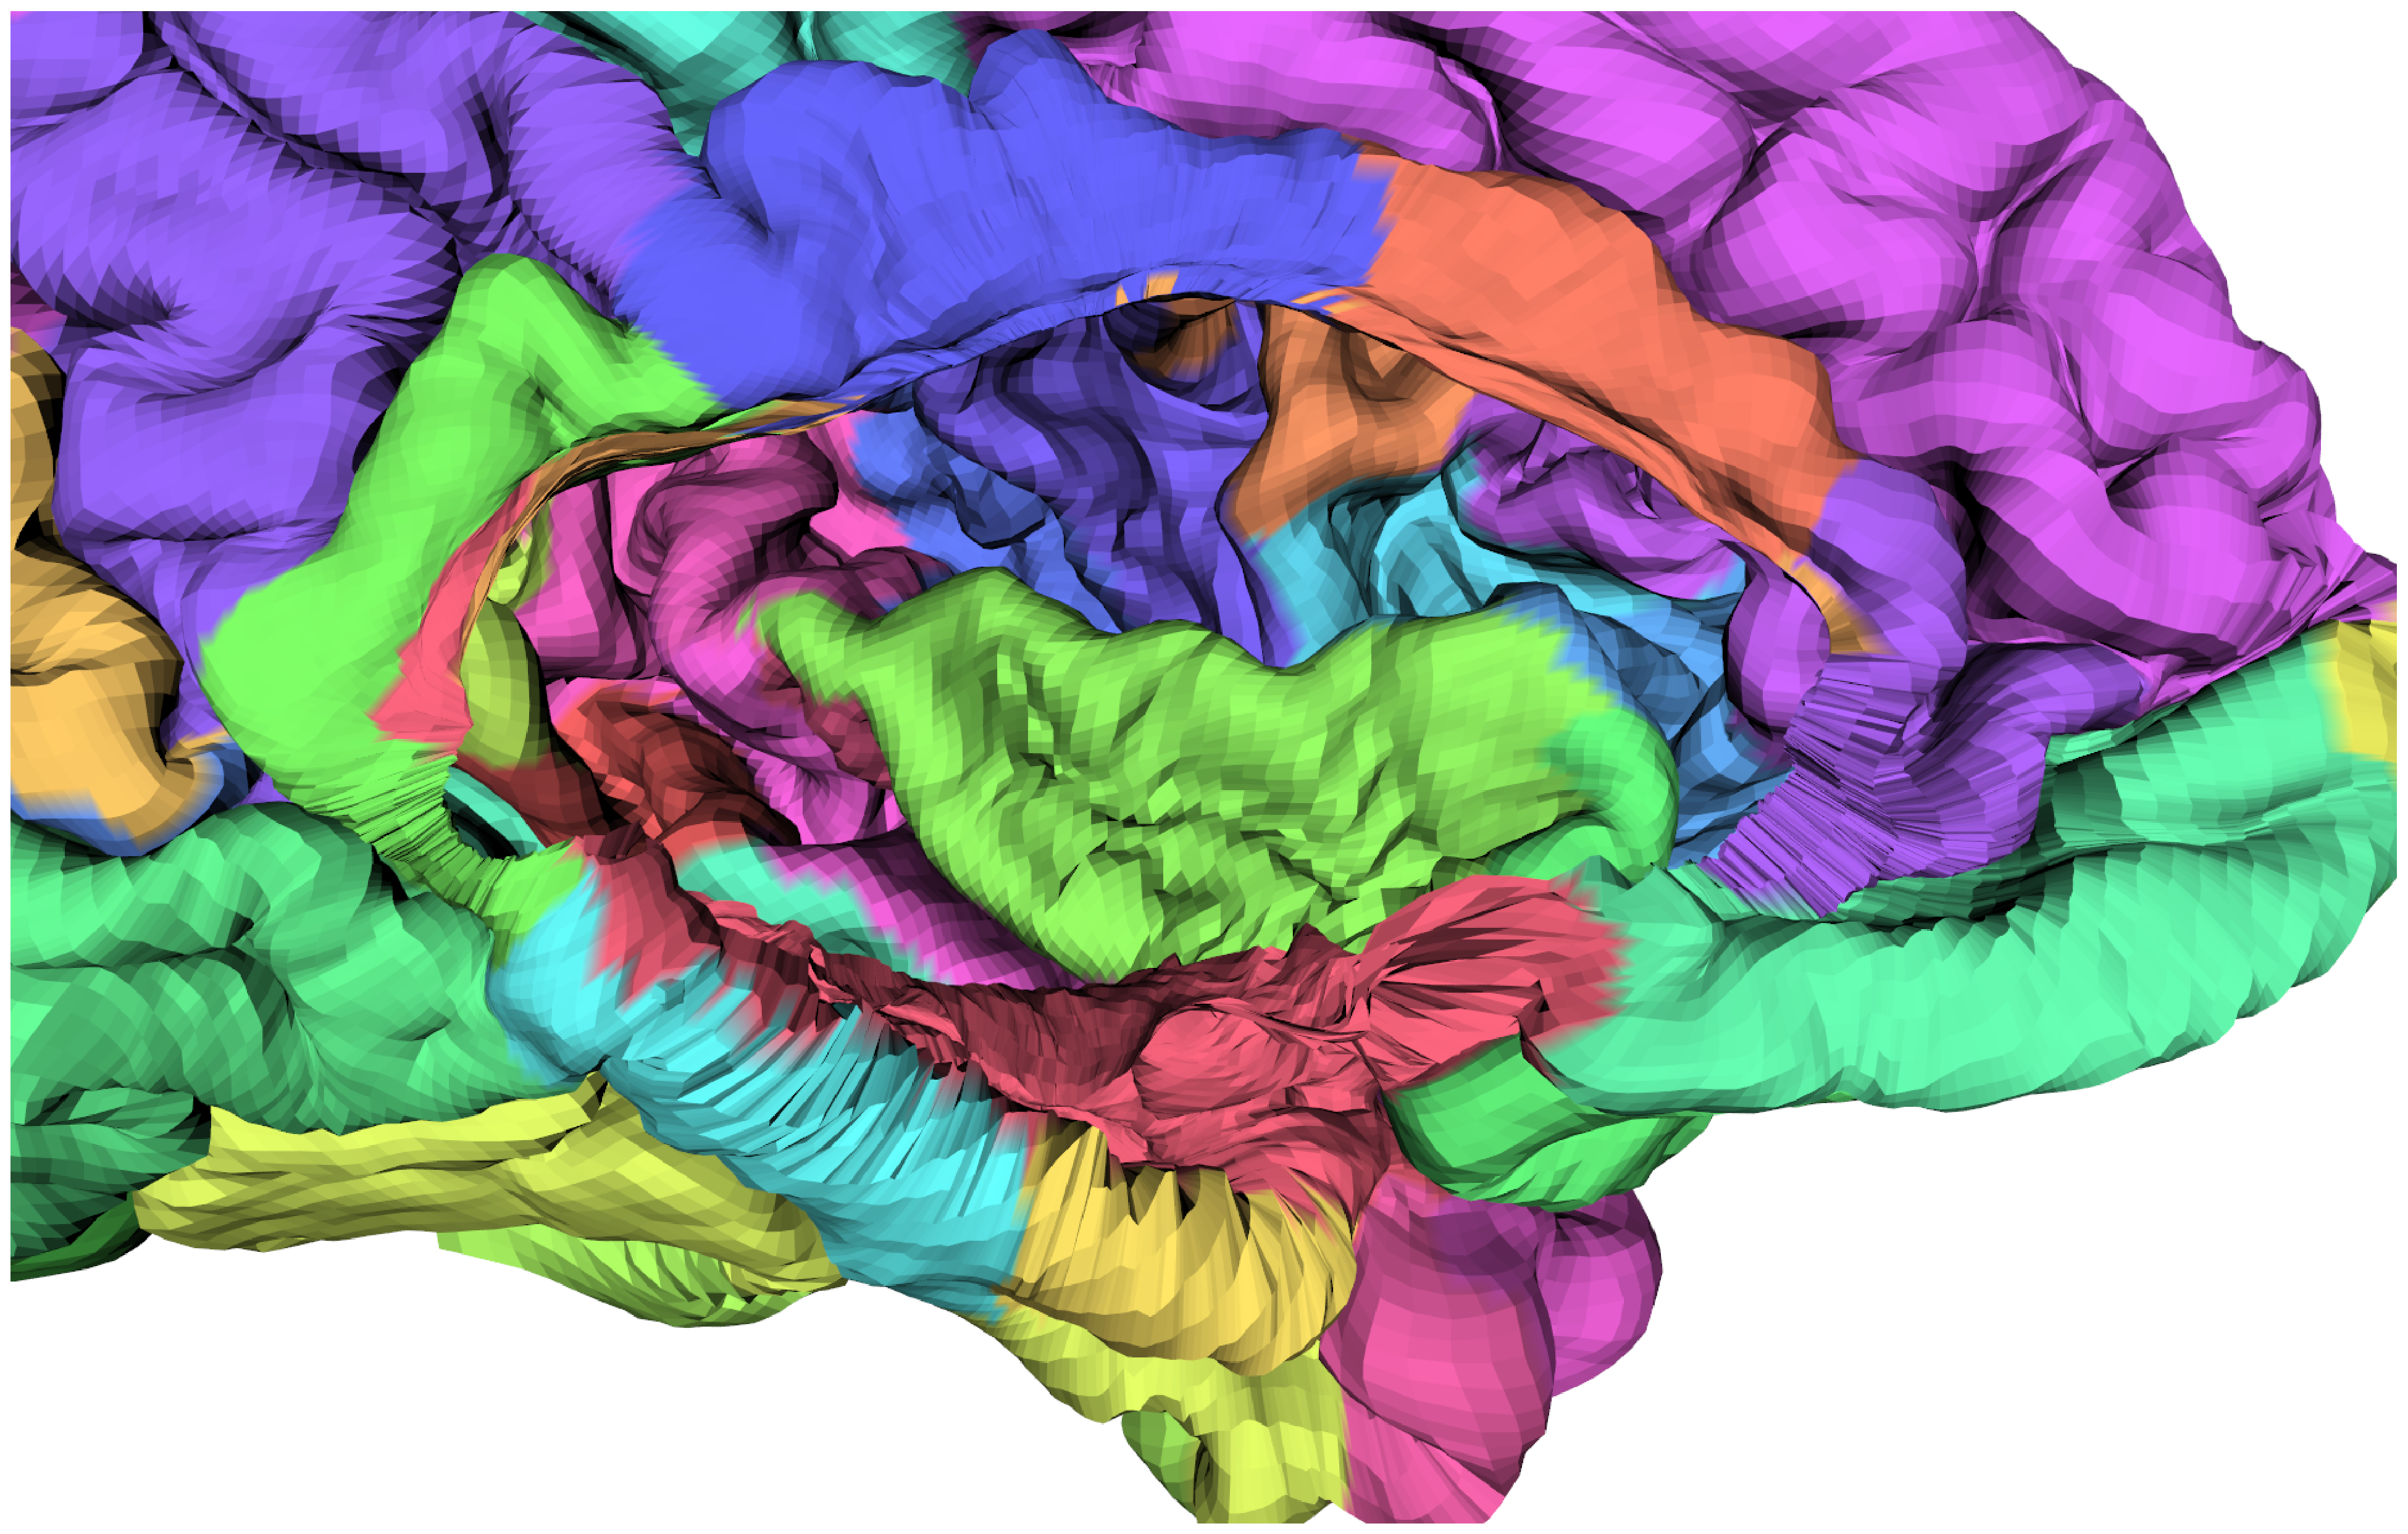
\epsfig{file = fittedSrepCircularGrid.eps, width = 3cm}}
% \subfigure[Square grid]{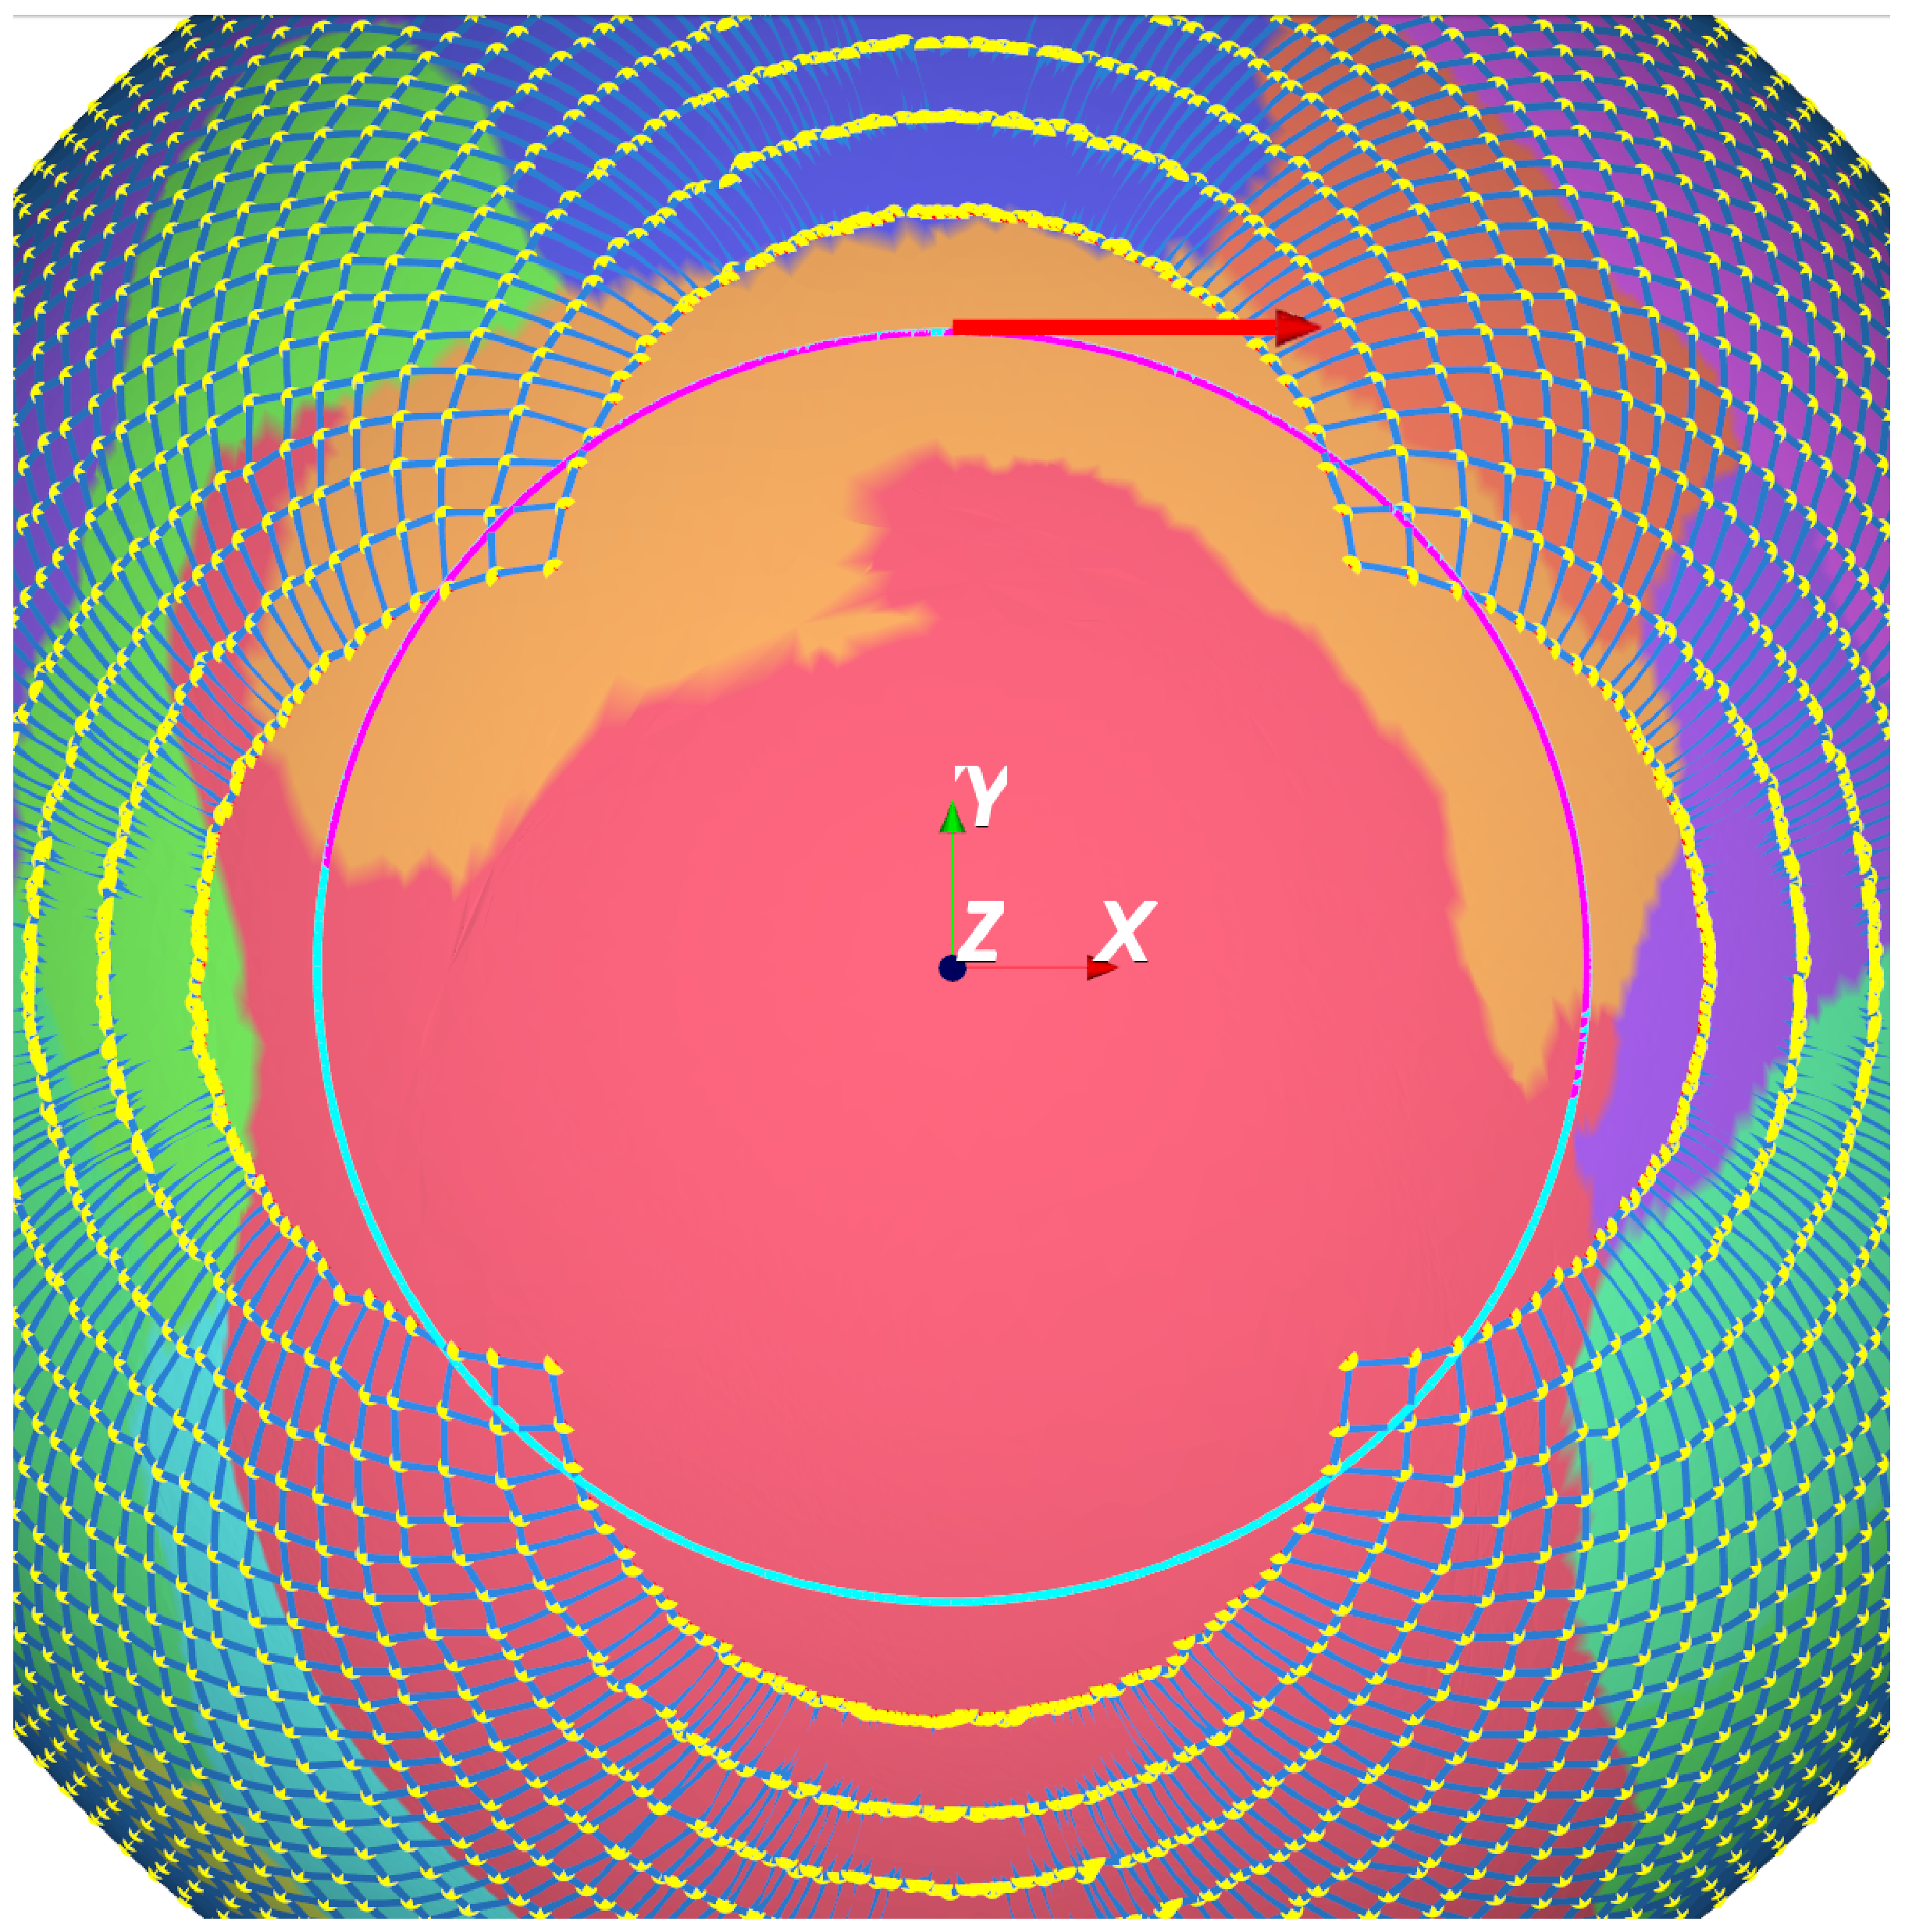
\epsfig{file = fittedSrepSphereSquareGrid.eps, width = 2.75cm} 
%		       \epsfig{file = fittedSrepSquareGrid.eps, width = 3cm}} 
% \caption{The best circle is shown in cyan, the projected points in magenta (on top of the best circle).
%	  The north pole is the center point of the best fitting circle, it is used to rotate the sphere to the north pole. 
%	  The mean of the projected points is found on the circle and is used to calculated a tangent, which is later used to 
%	  calculate a second rotation to align the data with the x axis. On figure (b), the regions highlighted in red correspond 
%	  to the corners of the grid.}
% \label{fig:BestCircle}  
%\end{figure}

The s-rep is folded into the cortex
using the points found on the sphere and
the cortical widths given by \textit{Freesurfer}. 

The following penalties minimize an objective function for each hub:

\begin{enumerate}
 \item The hub's distance to the GM and WM surfaces (~half the cortical width).
 \item The top spoke's tip distance to the GM surface.
 \item The bottom spoke's tip distance to WM surface.
 \item The normal of the SS (see Equation \ref{equ:sheetNormal}) to the normal of the WM surface.
 \item The normal of the SS to the normal of the GM surface.
\end{enumerate}


%\begin{equation}
% \hat{s_{rep}(i)} = \operatorname*{Arg\,min}_{p_i, s^{-1}_i, s^1_i} \sum_{j=1}^{k} || Cp(j) - p_i || + \left \{ \begin{array}{ll}
%                                                                                                                 ||Cp(j) - (p_i +  s^{-1}_i)||, & Cp(j) \in WM \\
%                                                                                                                 ||Cp(j) - (p_i +  s^{1}_i)||, & Cp(j) \in GM
%                                                                                                                \end{array} \right .
%                                                                                                     + || (s^{1}_i - s^{-1}_i) - NCp(i) ||
%\end{equation}

The procedure folds back the s-rep that was sampled on the spherical space to the original shape of the cortex. 
After the folding, the topology of the s-rep is preserved. 
In other words, each of the quads that build the skeletal structure 
are correctly oriented on the folded form of the cortex. 
Moreover, both top and bottom spokes point towards the GM and WM surfaces respectively. The width of the
spokes is also determined.

The interpolation mechanisms described in Section \ref{sec:s-repImplementation} can 
be used to produce the WM and GM surfaces. 
Since the implied surfaces are not equivalent to the original ones, the following section evaluates 
their quality. 

\section{Evaluation of the implied GM and WM surfaces}
\label{sec:Evaluation}

To evaluate if the surfaces are close enough to the original ones, 
a tool known as \textit{Meshvalmet} is used.
The tool uses the Hausdorff distance to estimate the difference between discrete 3D surfaces. 
The approach is based on \cite{aspert_mesh:_2002}. It
calculates the mean distance error from each vertex of the reference surface to 
a target one, in this case, the interpolated surface against the original surface. 
The comparison is done separately on the GM and WM surfaces.
The sampling step is set to $0.1$ and an absolute distance measure is used.
By lowering the sampling step and using the 
absolute distance, the accuracy of \textit{Meshvalmet} is increased.

Analyzing the results of \textit{Meshvalmet} 
yields a set of parameters to generate the best possible representation 
for all subjects. 
The parameters to set for the s-rep are size and sampling step on the sphere.
The following section analyzes the size of the s-rep.

\subsection{Best s-rep size}
\label{sec:s-repsize}

\begin{figure}[!h]
 \centering 
 \subfigure[GM surface]{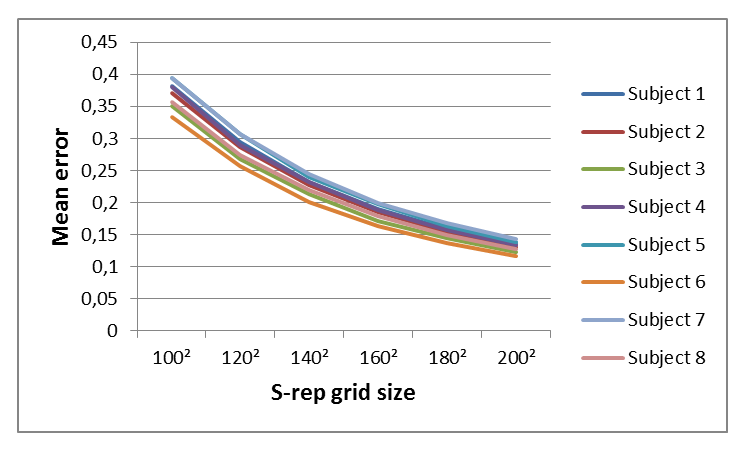
\epsfig{file = lh_greyMatterGridSize.eps, width = 7.25cm}}
 \subfigure[WM surface]{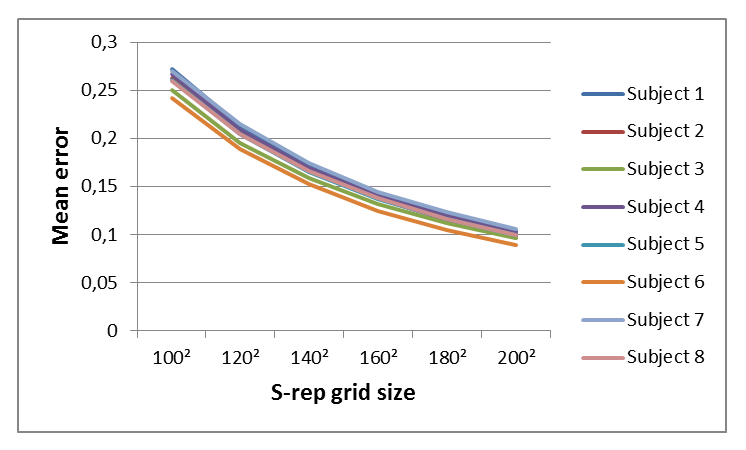
\epsfig{file = lh_whiteMatterGridSize.eps, width = 7.25cm}}
 \caption[GM and WM surface mean error: grid size.]{Mean error using different grid size of the s-rep.}
 \label{fig:GridSize} 
\end{figure}

The first parameter to set is the size of the s-rep. This is based on different criteria
such as reducing the number of points in the original data. A typical cortical surface contains $130,000+$ vertex.
By using an s-rep of $160^2$ atoms, the information is reduced by $~40\%$, \textit{i.e}, 
$76.800$ tuples including the hub positions plus both spoke directions.
%Reducing the information not only allows to produce compact representation of the data but it also allows the use of new statistical tools.

Figure \ref{fig:GridSize} shows the mean error using s-reps of different sizes, tested on 8 different subjects. 
The following analysis uses a grid of $160^2$ atoms for all cases.

\subsection{Best s-rep sampling}
\label{sec:minvalue}

The second parameter to set is the initial value for the log scale sampling on the grid.
This parameter controls how the hubs will distribute on the sphere. A value close to $0$ will 
map a larger number of points towards the south pole. 
Figure \ref{fig:AverageCell} shows the average area of the quads that compose the skeletal locus of the s-rep and their SD (standard deviation).
Notice that for values greater that $0.04$, the SD increases rapidly.
Figure \ref{fig:InitialLogValue} shows the mean error of the interpolated surfaces for different $Min$ values.
According to the analysis, values between $0.01$ and $0.4$ seem reasonable as 
the minimum error overall cases for the surfaces is found inside this range.
The $Min$ value is set to $0.02$
in order to increase the regularity of the quads and 
lower the mean error of the surface.
This value produces the best results over all subjects used in the analysis. 

\begin{figure} 
 \centering  
 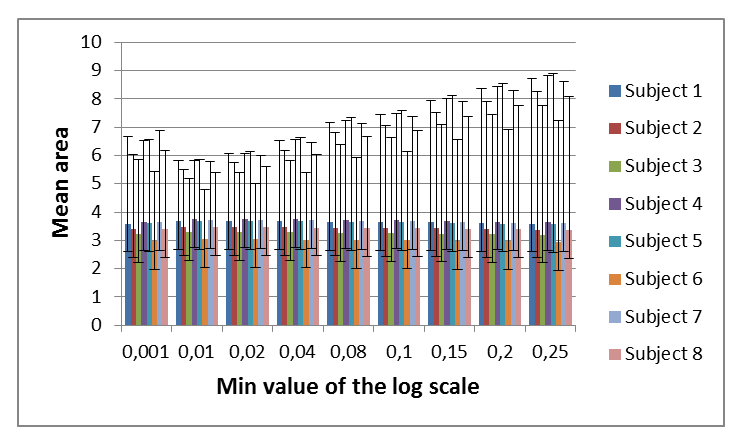
\epsfig{file = lh_averageCellArea.eps, width = 9cm}
 \caption[Average area of an srep's quad.]{Average quad area of the s-rep with standard deviation for different $MIN$ values of the log scale.}
 \label{fig:AverageCell}  
\end{figure}

\begin{figure} 
 \centering 
 \subfigure[GM surface]{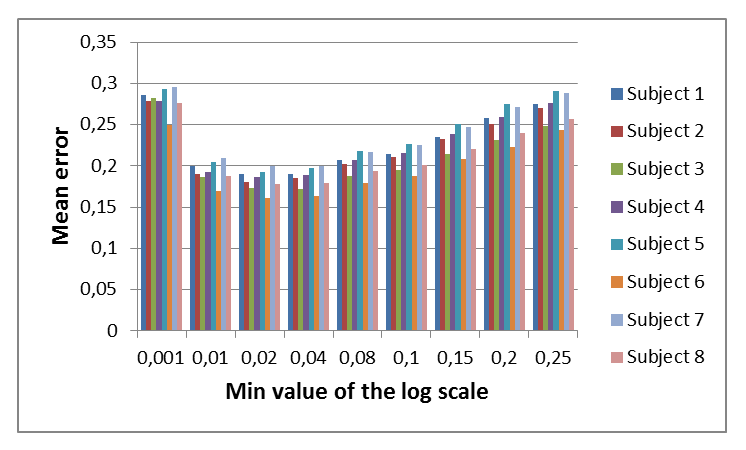
\epsfig{file = lh_greyMatterLogScale.eps, width = 7.25cm}}
 \subfigure[WM surface]{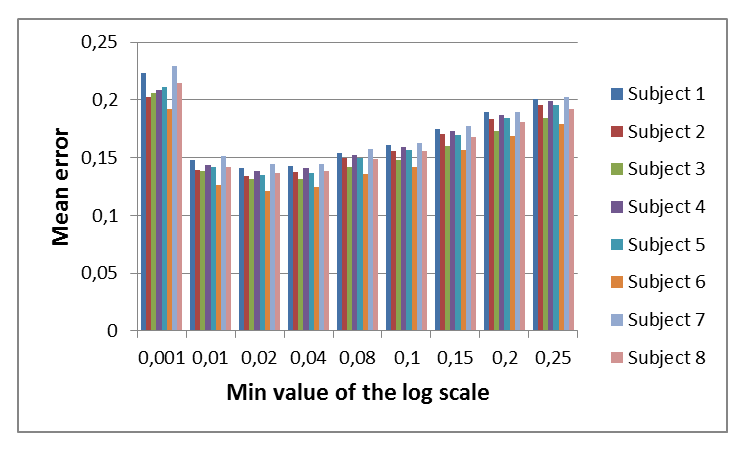
\epsfig{file = lh_whiteMatterLogScale.eps, width = 7.25cm}}
 \caption[GM and WM surface mean error: log scale.]{Mean error of the GM and WM surfaces for different $MIN$ values of the log scale.}
 \label{fig:InitialLogValue} 
\end{figure}


Figure \ref{fig:InterpolatedCortex} shows the interpolated cortex for both hemispheres. 
The coloring on the surfaces are set according to the cortical
parcellation of the neuroanatomical structures at each location in the cortex. 
%Each atom has the corresponding label found on the spherical surface.
%During the interpolation, each new point is labeled according to a voting scheme using the labels of the closest neighboring atoms.

\begin{figure}
 \subfigure[Original surfaces.]{\epsfig{file = lh_whiteMatterOriginal.eps, width = 8cm}
			   \epsfig{file = rh_whiteMatterOriginal.eps, width = 8cm}}
 \subfigure[Interpolated surfaces.]{\epsfig{file = lh_whiteMatterInterpolated.eps, width = 8cm}
			   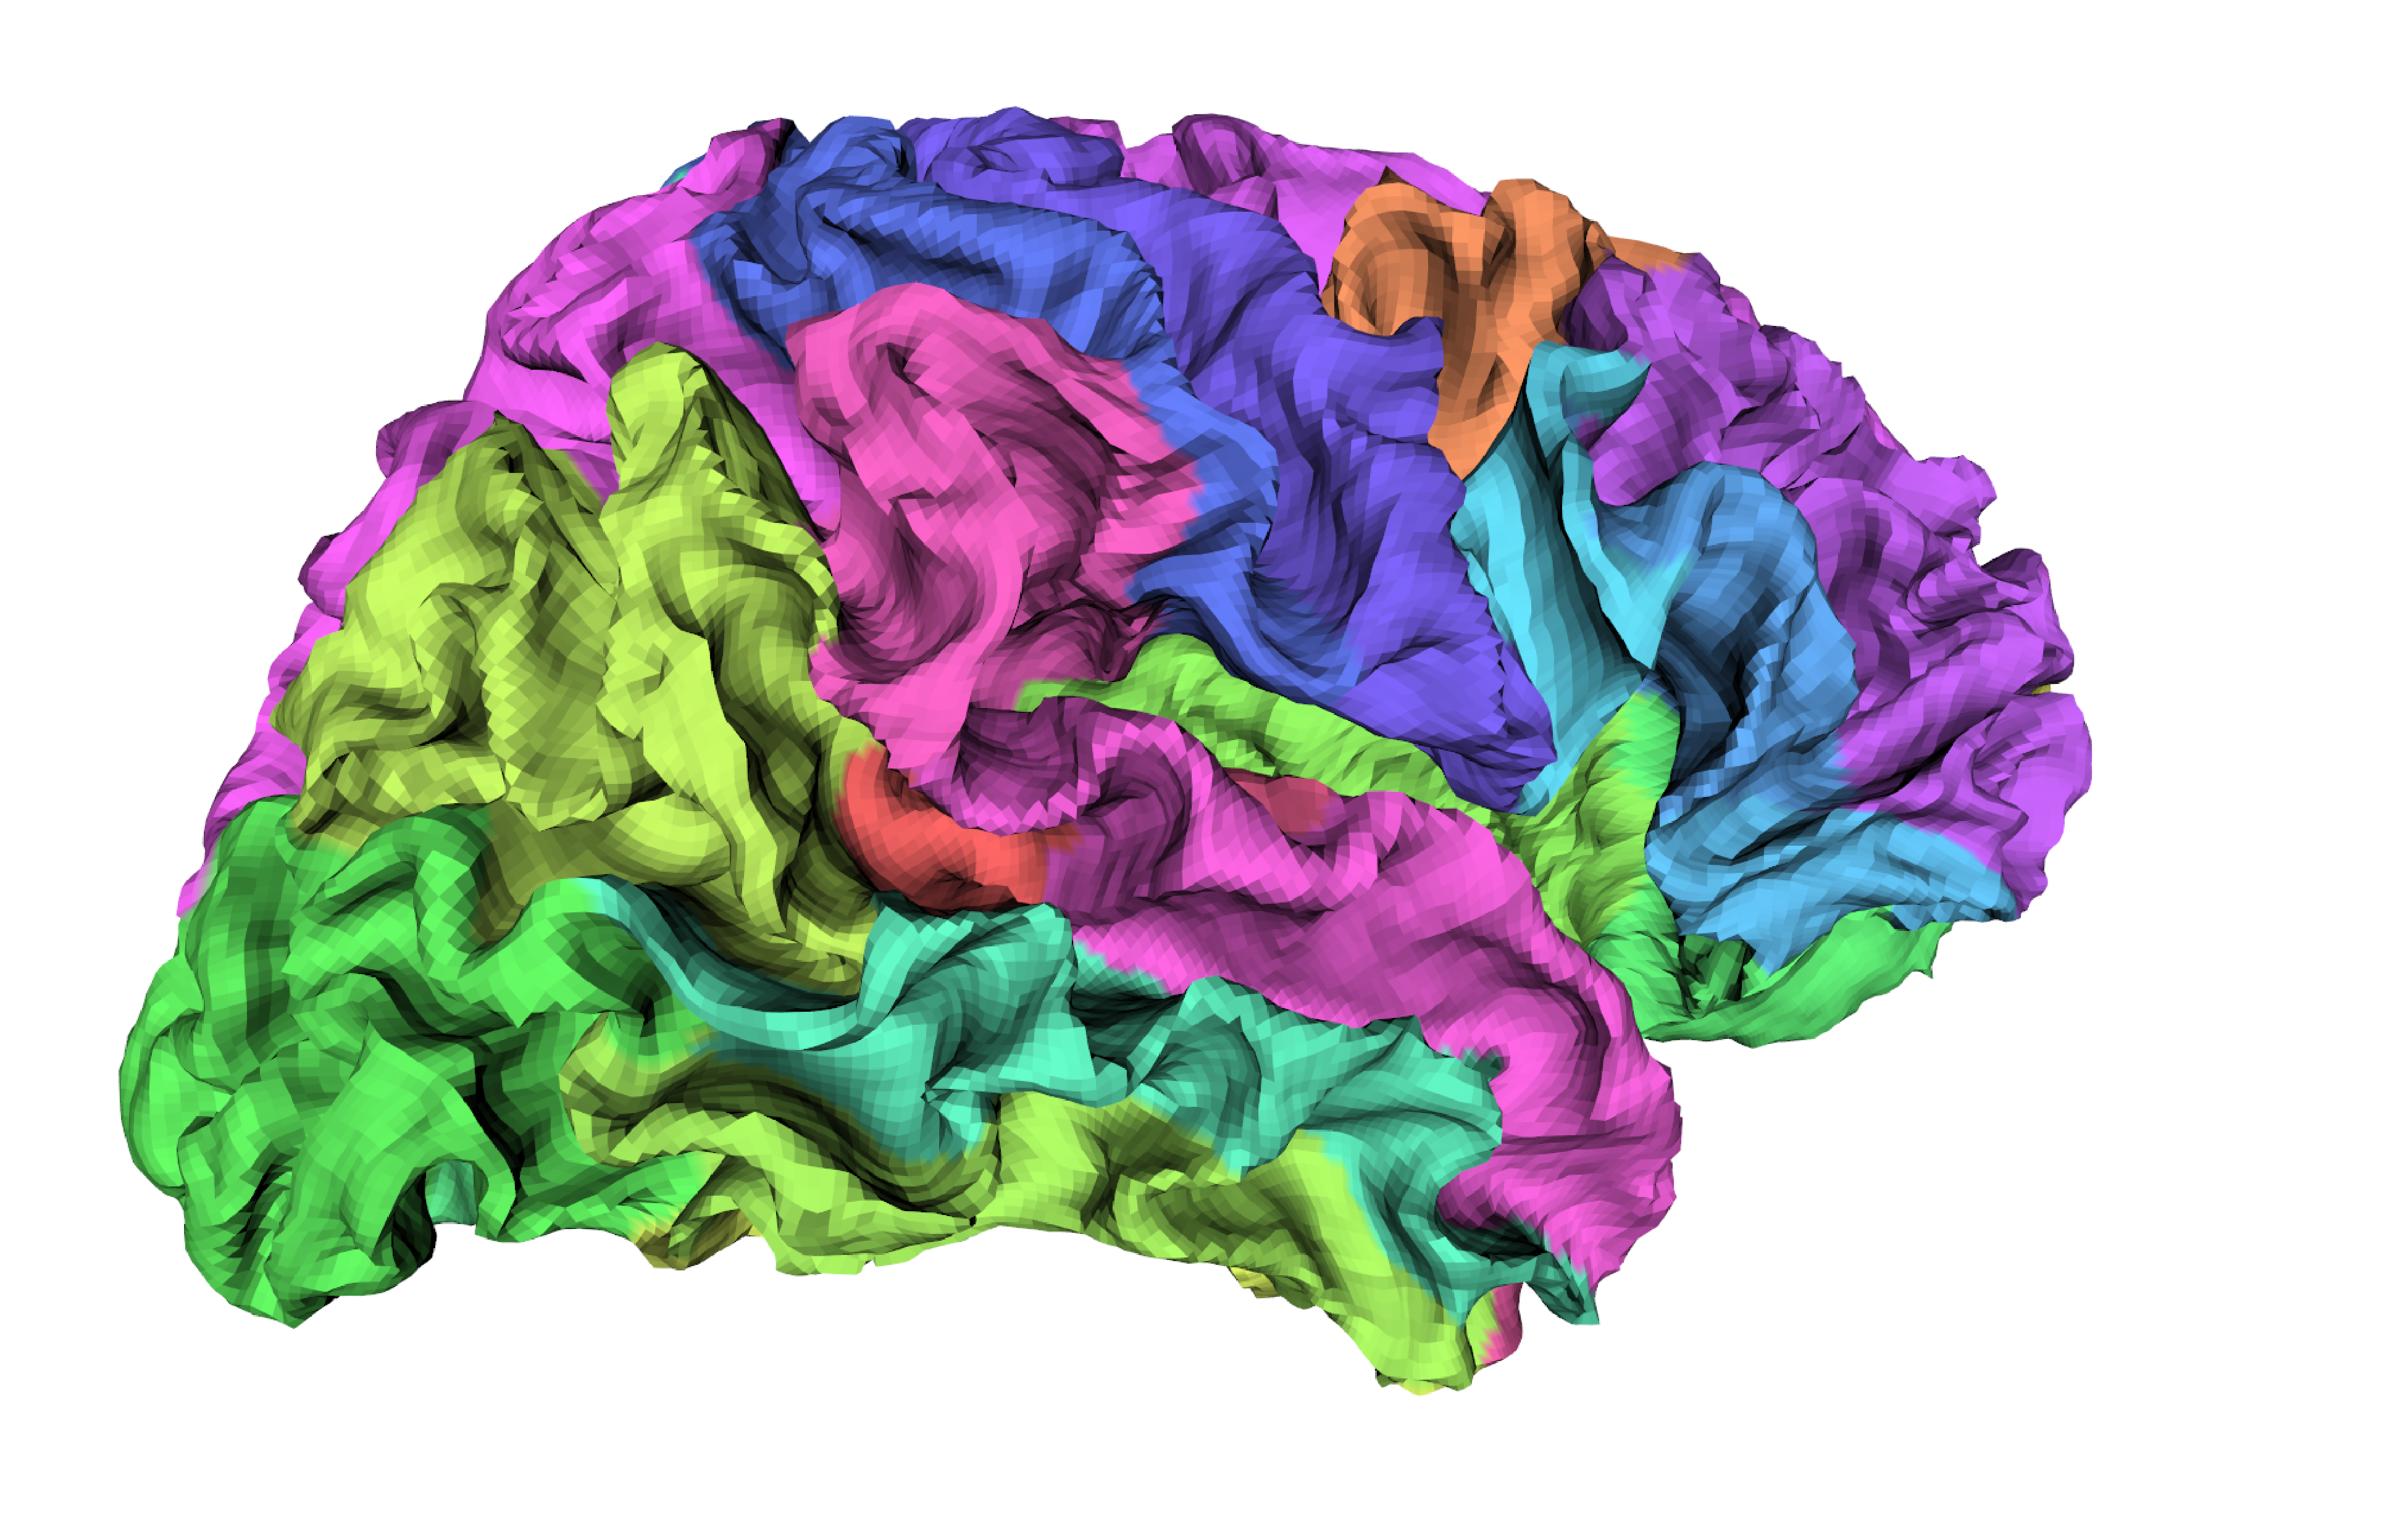
\epsfig{file = rh_whiteMatterInterpolated.eps, width = 8cm}}
 \caption[Comparison of the interpolated and original WM surfaces.]{Comparison of the original and interpolated WM surfaces for the left and right hemispheres.
	  The s-rep has $160^2$ atoms. The interpolated surfaces seem to have wrinkles at some places 
				      but according to the error measurement, they are close to the original ones. 
	                             Moreover, modeling the cortex via s-reps offers new capabilities such as the local coordinate system inside the structure.
	                             This new set of capabilities are not available in the regular representation.}
 \label{fig:OriginalCortex}
\end{figure}
\begin{figure} 
 \subfigure[Original surfaces.]{\epsfig{file = lh_greyMatterOriginal.eps, width = 8cm}
				  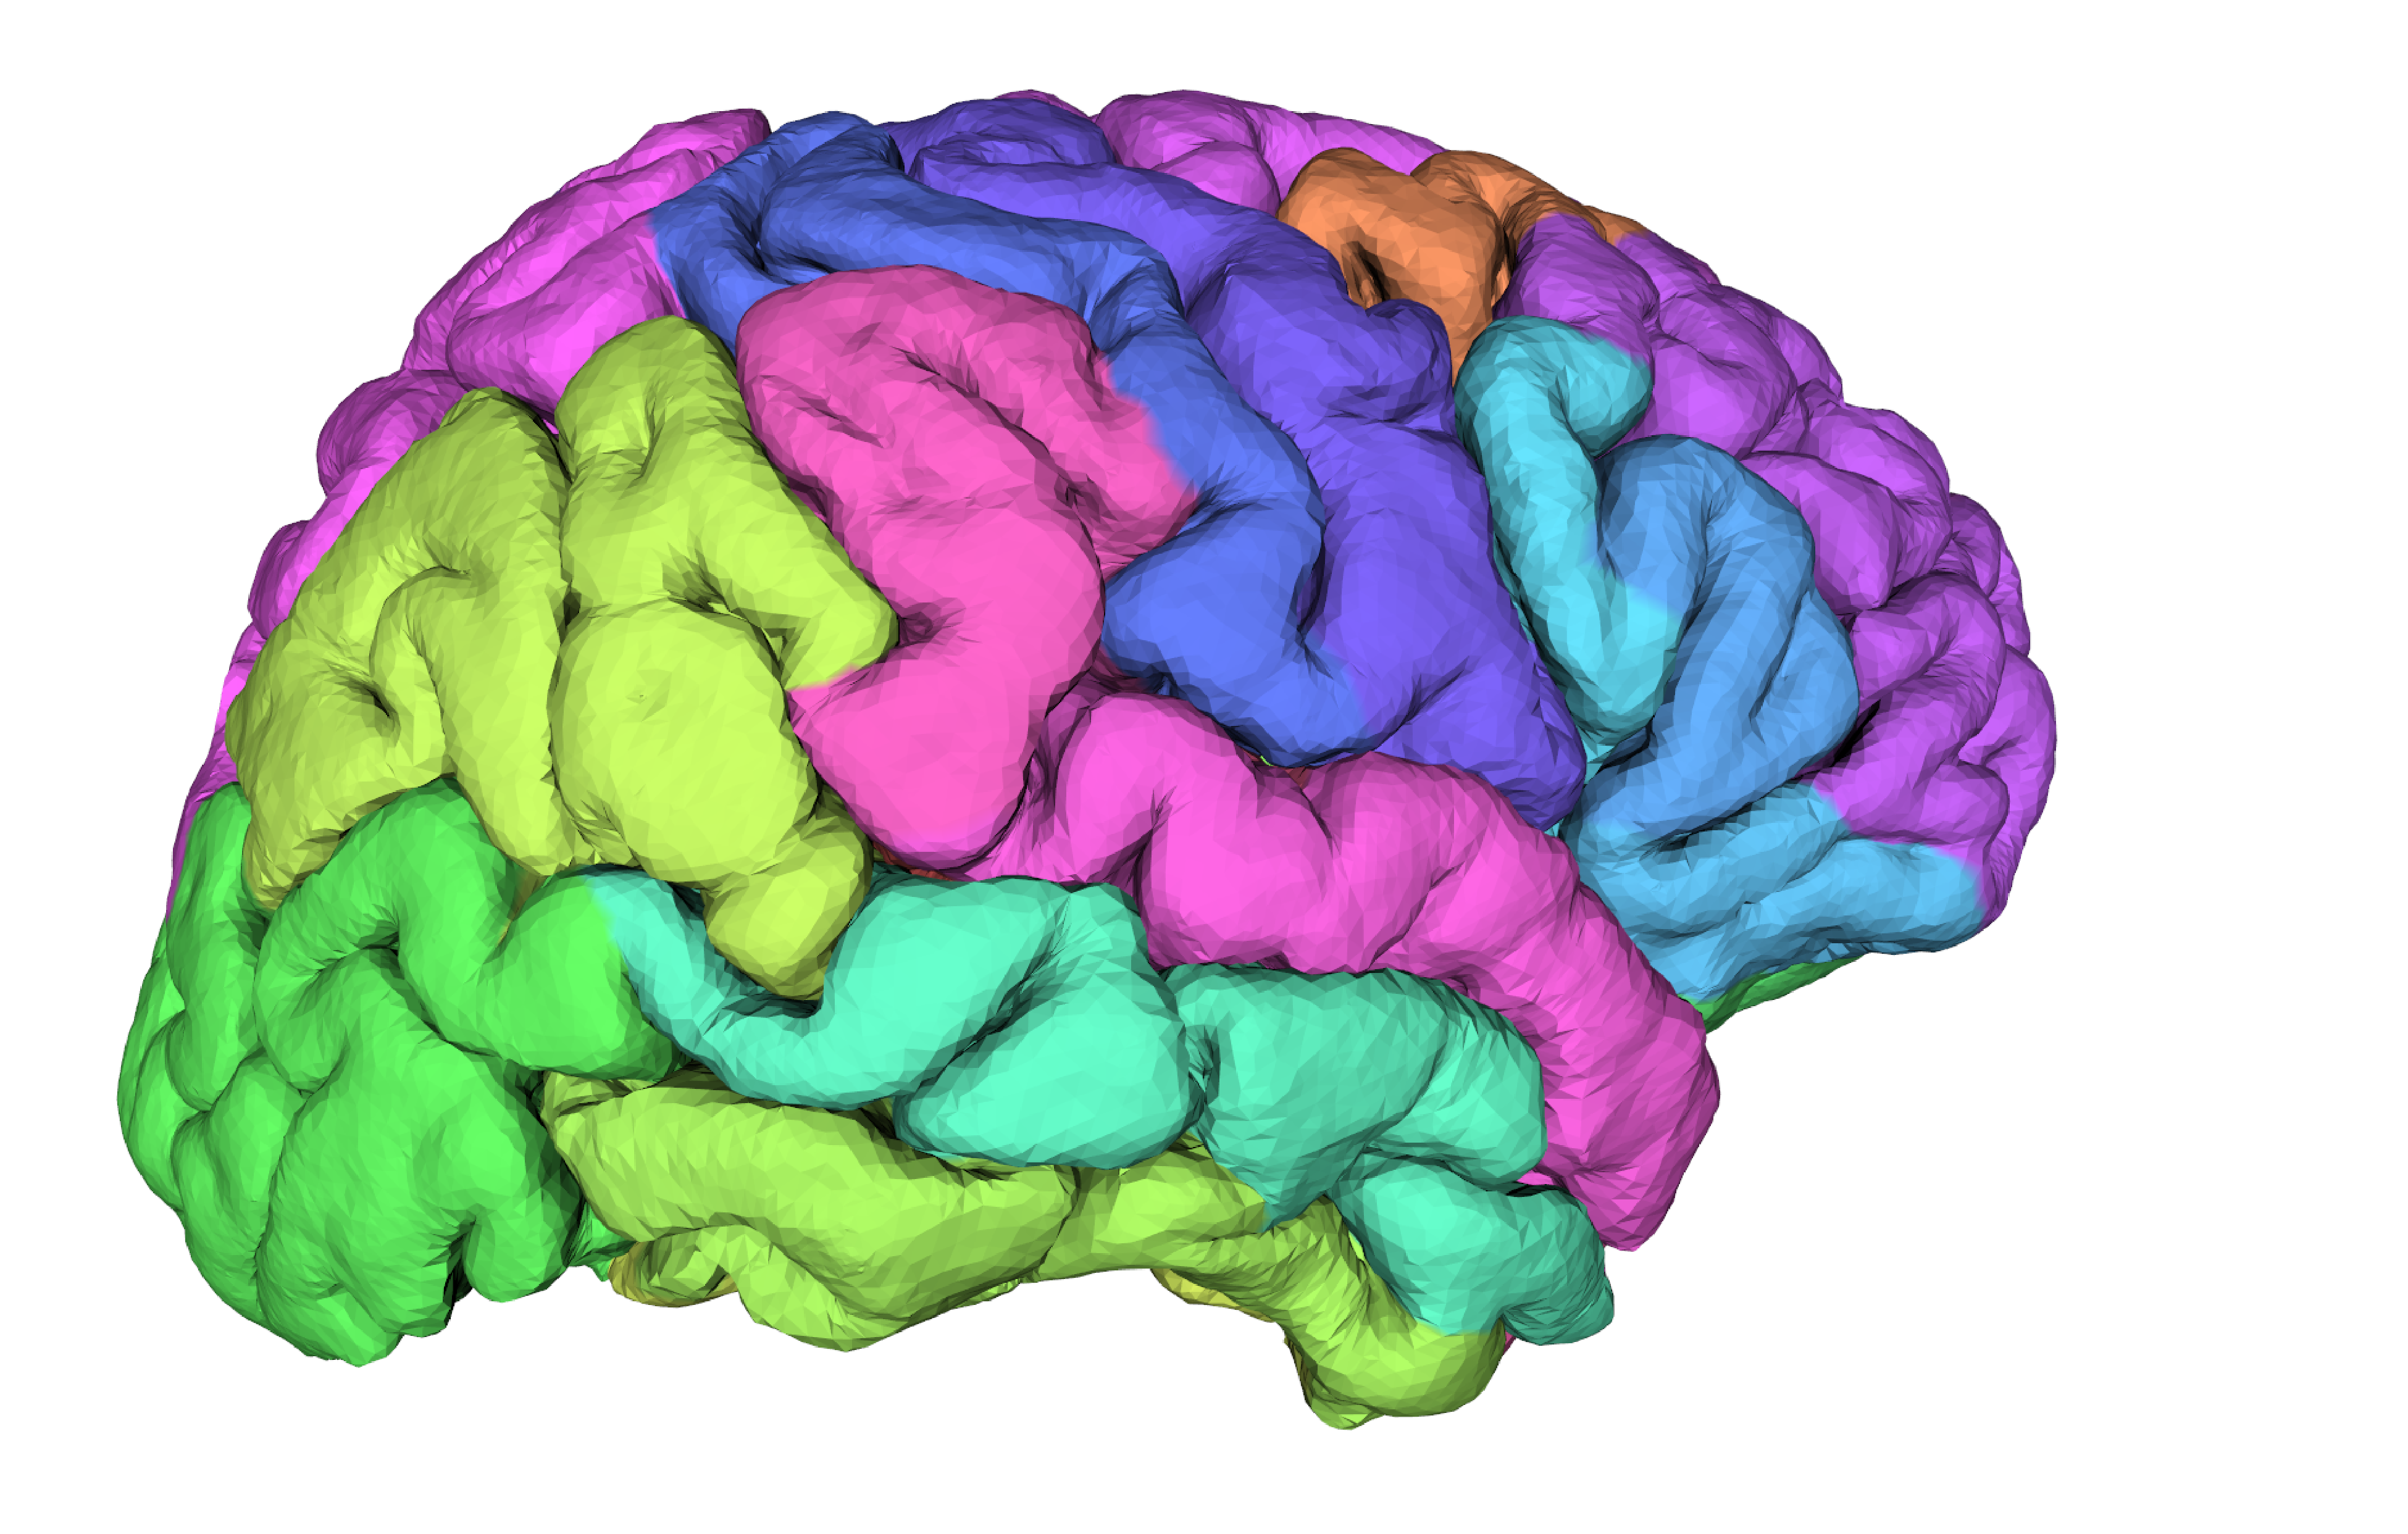
\epsfig{file = rh_greyMatterOriginal.eps, width = 8cm}}
 \subfigure[Interpolated surfaces.]{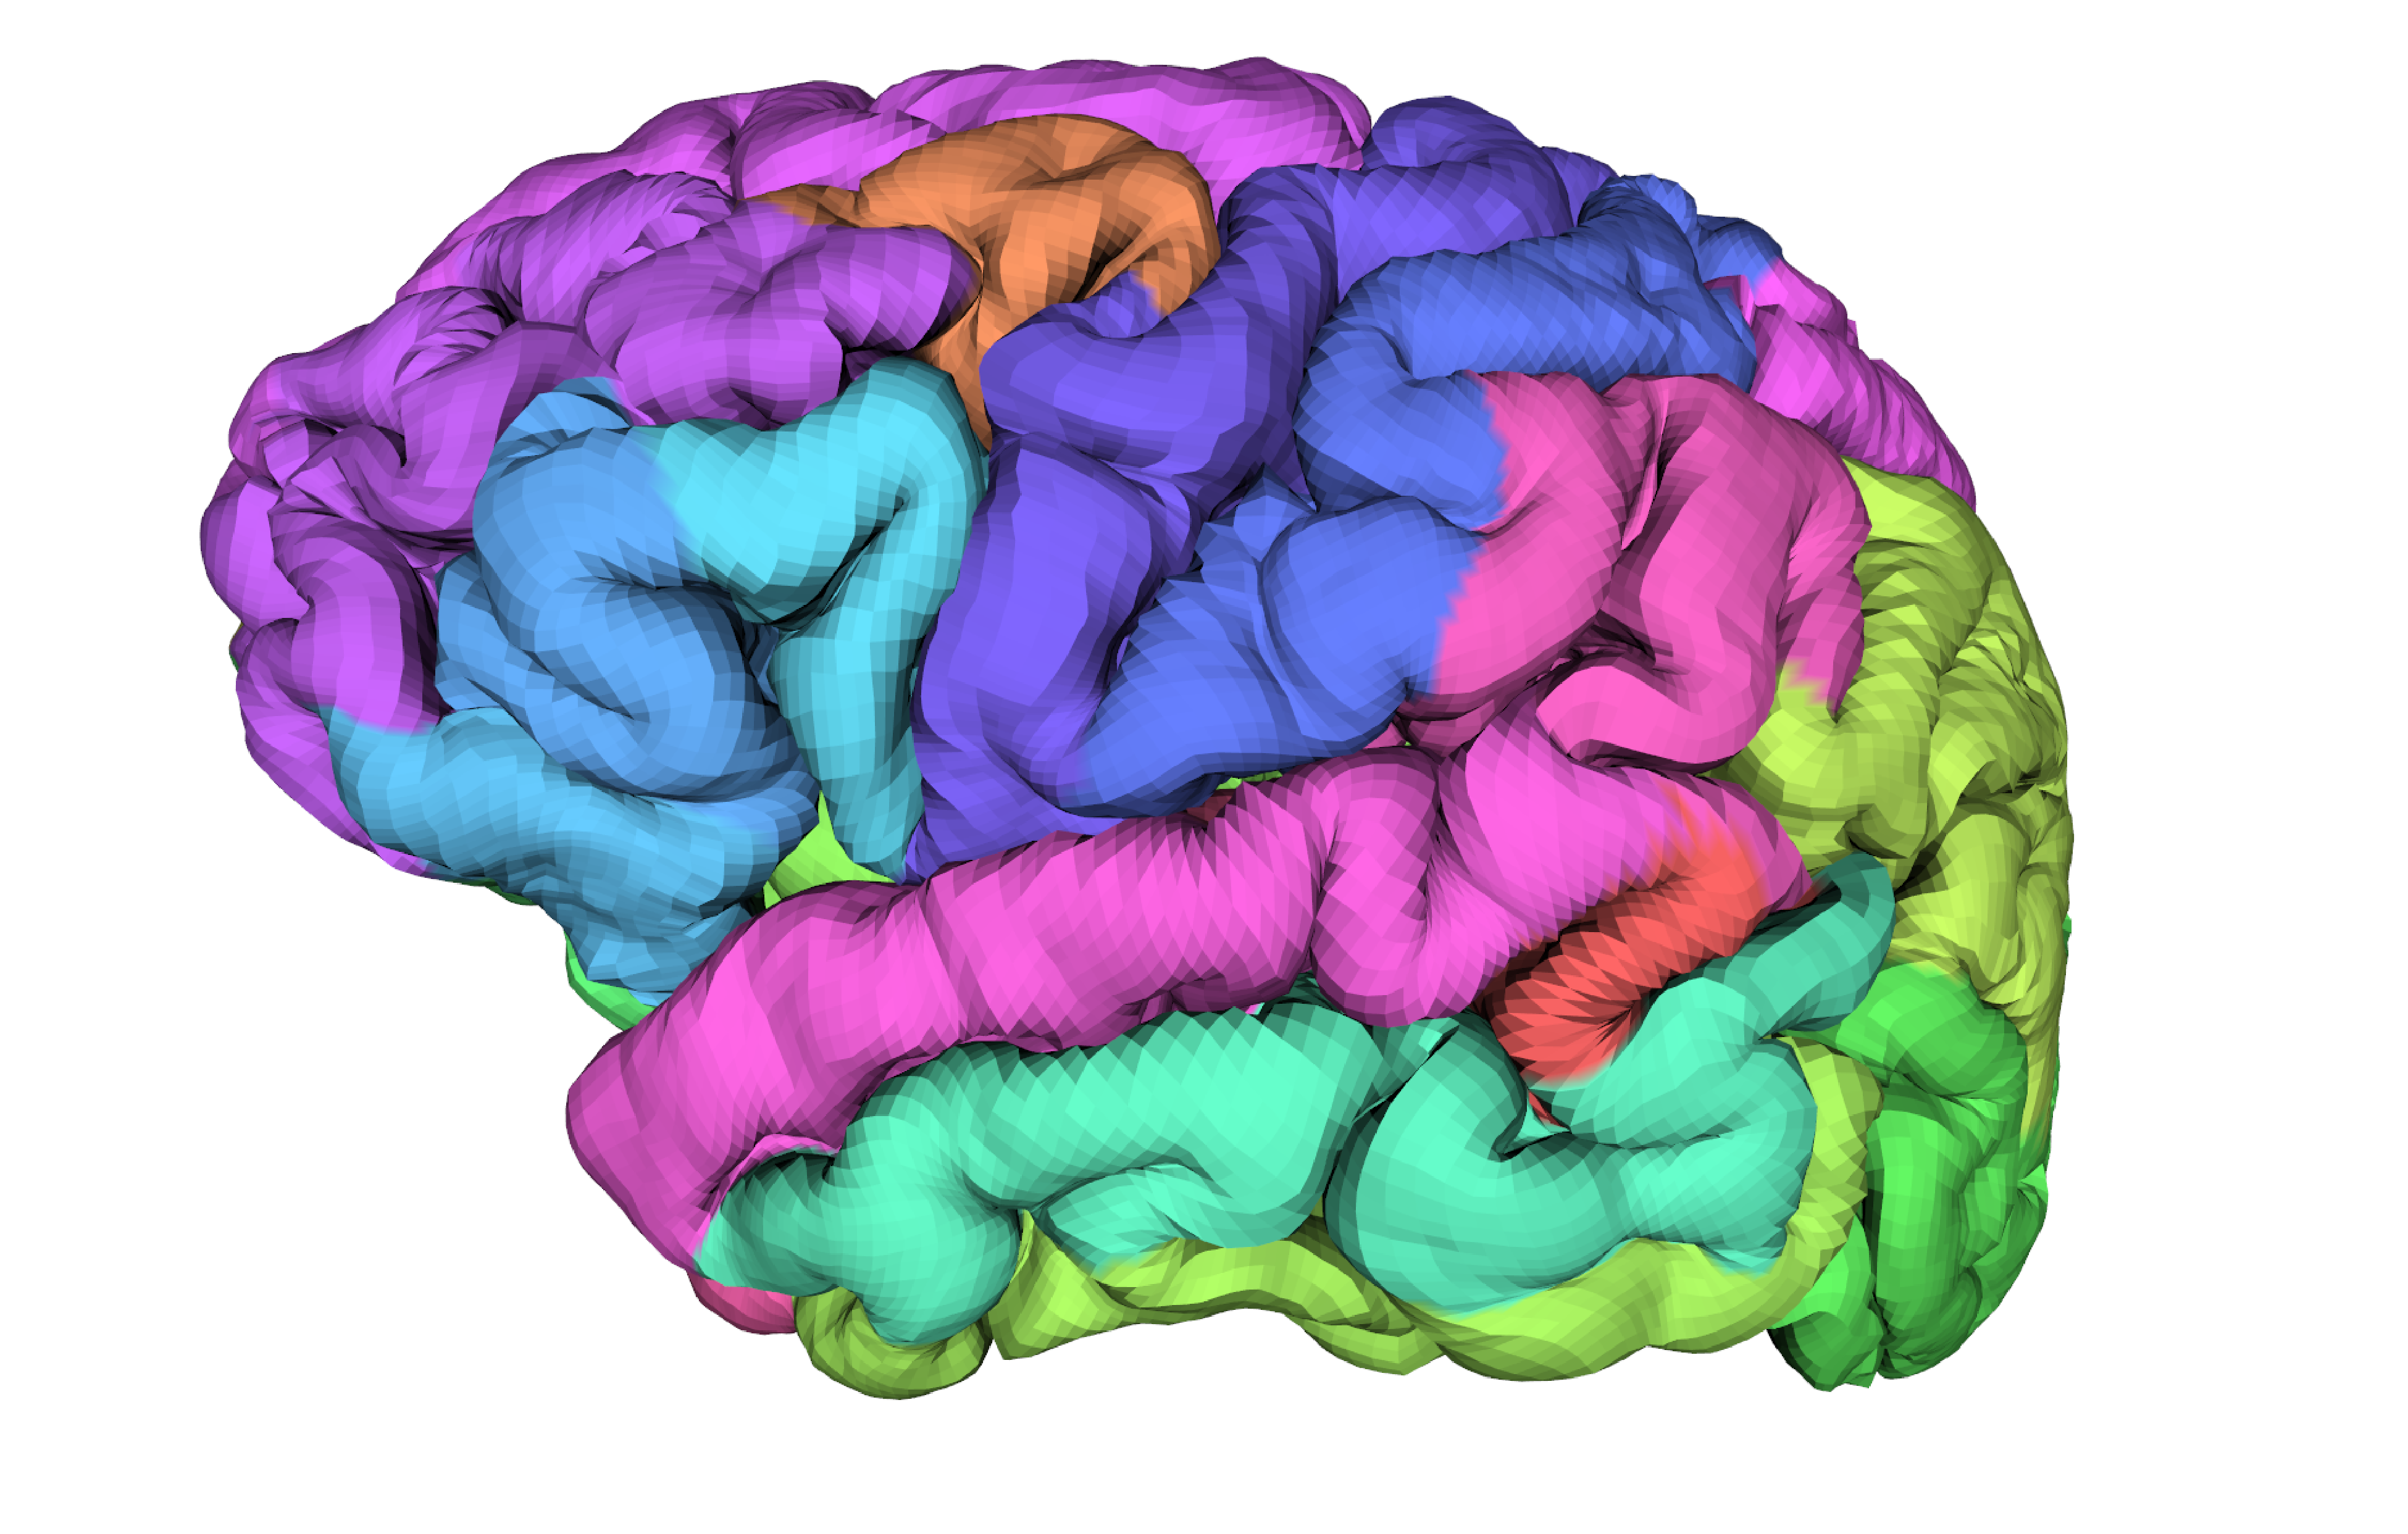
\epsfig{file = lh_greyMatterInterpolated.eps, width = 8cm}
				  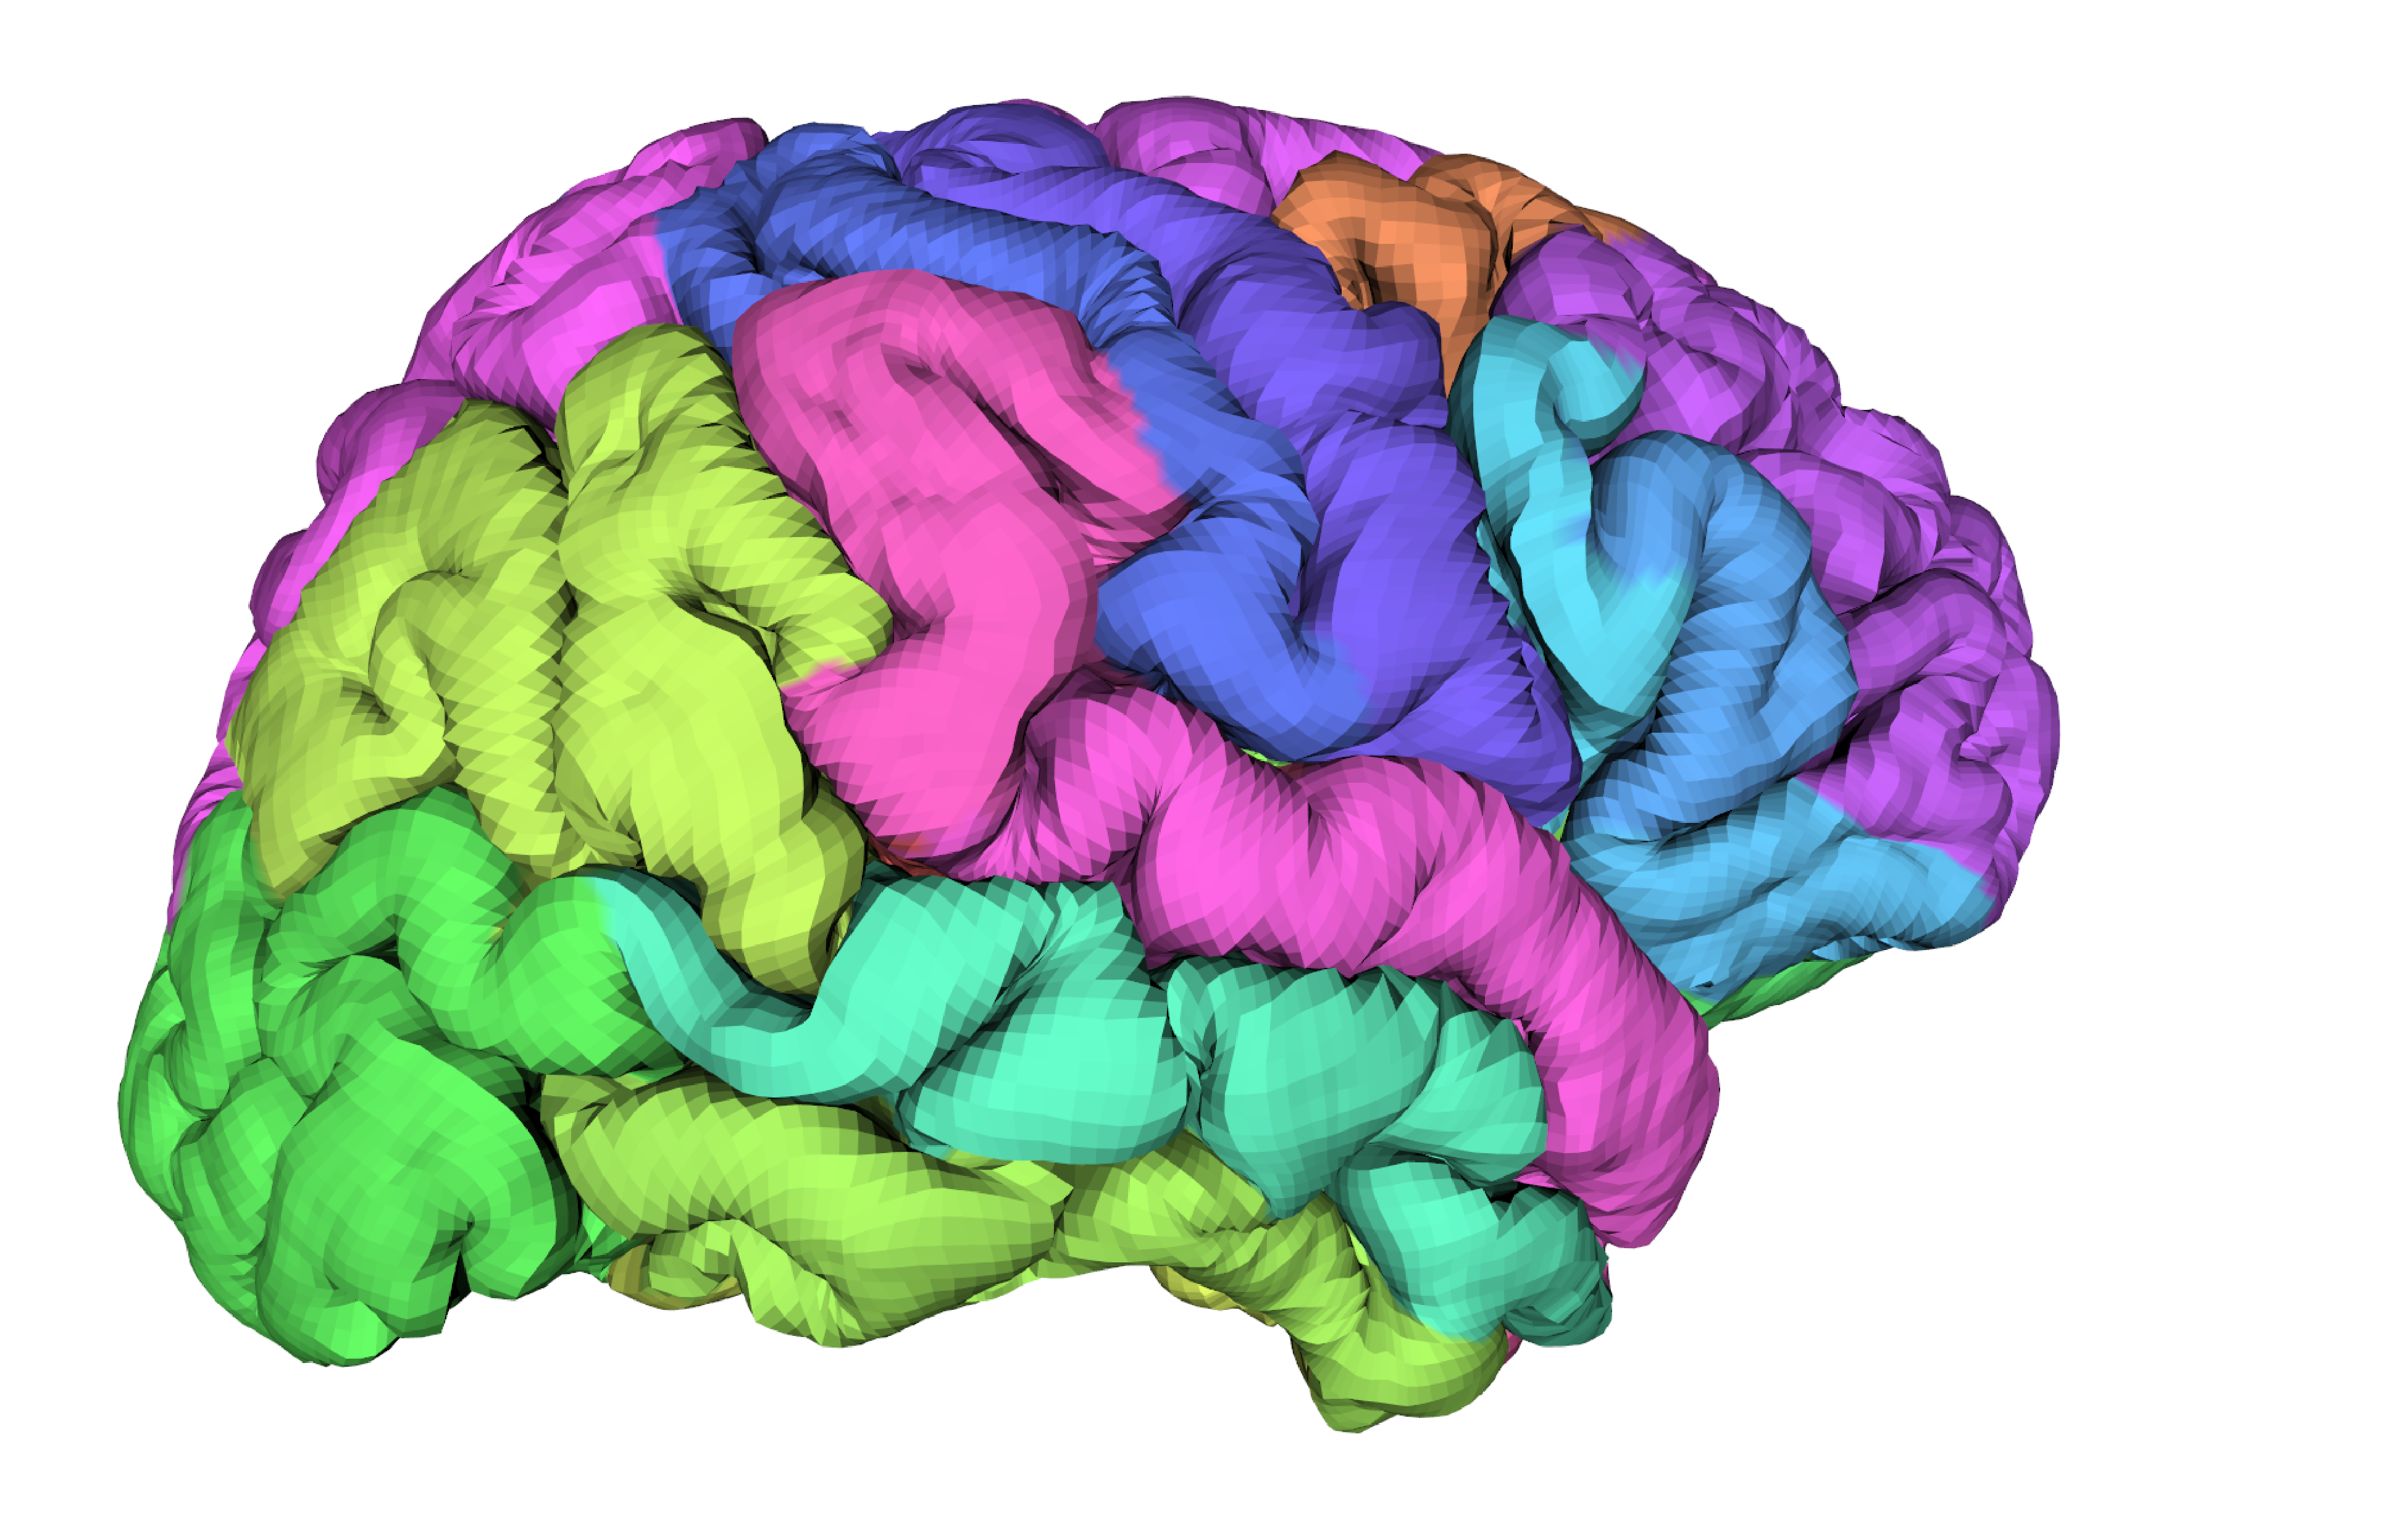
\epsfig{file = rh_greyMatterInterpolated.eps, width = 8cm}}
 \caption[Comparison of the interpolated and original GM surfaces.]{Comparison of the original and interpolated GM surfaces for the left and right hemispheres.			
	The s-rep has $160^2$ atoms. The interpolated surfaces seem to have wrinkles at some places 
				      but according to the error measurement, they are close to the original ones. 
	                             Moreover, modeling the cortex via s-reps offers new capabilities such as the local coordinate system inside the structure.
	                             This new set of capabilities are not available in the regular representation.}
 \label{fig:InterpolatedCortex}  
\end{figure}

In the following section, the s-rep of the cortex is used to evaluate
the changes of cortical width using synthesized data from a base model. 

%\begin{figure}
% \vspace{-0.2cm}
% \centering 
% \subfigure[Gray matter surface]{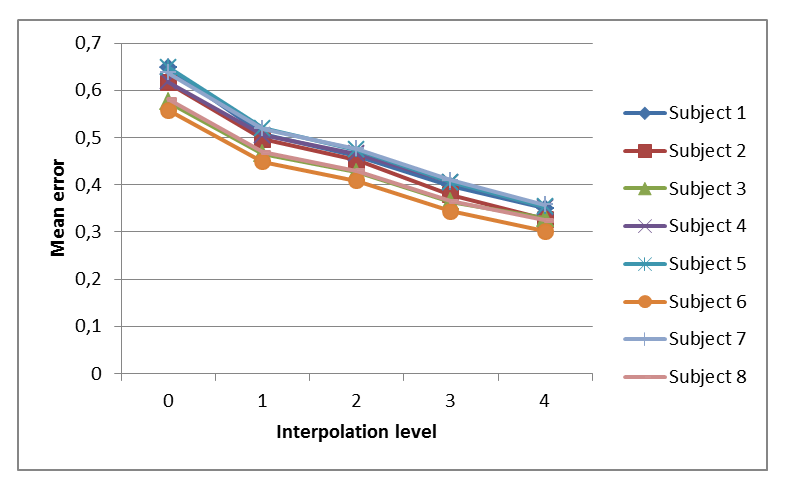
\epsfig{file = lh_greyMatterInterpolationLevel.eps, width = 6cm}}\\
% \subfigure[White matter surface]{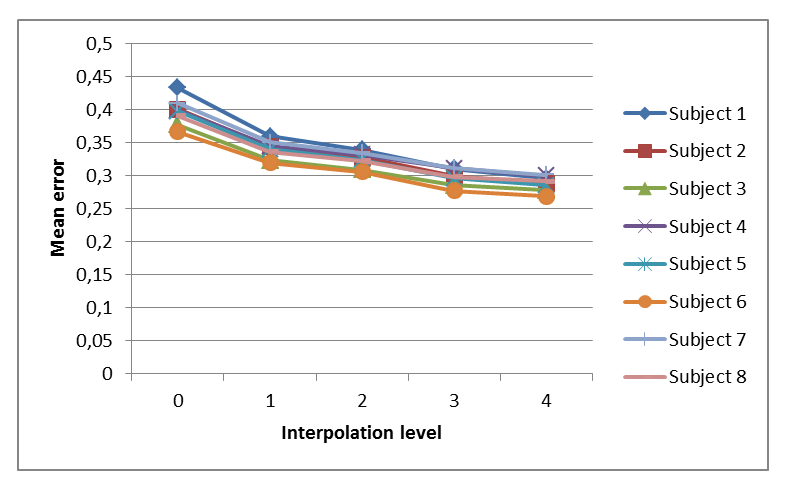
\epsfig{file = lh_whiteMatterInterpolationLevel.eps, width = 6cm}}
% \caption{Mean error for different start points of the log scale.}
% \label{fig:InterpolationLevel}
% \vspace{-0.1cm}
%\end{figure}

\section{Shape statistics of the cortex using CPNS}
\label{sec:Statistics}

%Statistics on objects has been applied to quite a variety of types of geometric model derived from the boundary
%cases:
%1. PCA has been applied to boundary point distribution models (\cite{cootes_training_1992}, \cite{kurtek_parameterization-invariant_2011}). 
%Kendall \cite{kendall_shape_2009} showed this is not correct as this type of models live in a space
%formed by a Cartesian product of a Euclidean space and high dimensional spheres. 
%Further developments yield a technique called PGA (principal geodesic analysis) \cite{angeles_generalized_2010} 
%which produced better statistics than PCA but still not satisfactory. 
%2.
%Deformation-of-atlas models, where the displacement of each voxel in the atlas
%is provided \cite{pennec_statistical_2009}, \cite{arsigny_log-euclidean_2006}). These models have enormous dimension, 
%and the statistical analysis is expensive and unstable with respect to the sampling
%into training cases and to noise in those training cases.
%3.
%Implicit models, such as level surfaces of pseudo-signed-distance functions \cite{clark_automatic_1998},
%that do not live in Euclidean feature spaces but are often analyzed (by PCA) as if they did.
%4.
%Skeletal models such as s-reps, live in abstract manifolds that are curved, 
%composed by a Cartesian product of a Euclidean space and a collection of spherical spaces.
%This type of models have many advantages as they capture information of the surface
%and the interior of the object by providing a local frame and a coordinate system
%created from the atoms sampled on the medial sheet. 
S-reps live in abstract manifolds that are curved,
composed by a Cartesian product of a Euclidean space and a collection of spherical spaces.
Using s-reps to compute shape statistics should yield better shape descriptors as volumetric information
is included into the analysis. 
Previous studies on s-reps of hippocampi have shown 
CPNS to yield lower-dimensional shape space with an efficient collection of modes of variation better than 
PCA-based statistical analysis of other skeletal or non skeletal models \cite{pizer_nested_2012}, \cite{schulz_2012}.
The analysis on the cortex is challenging since its dimension is very high and shape variations could go undetected
by the approach.

\begin{figure}[tb]
  \centering
  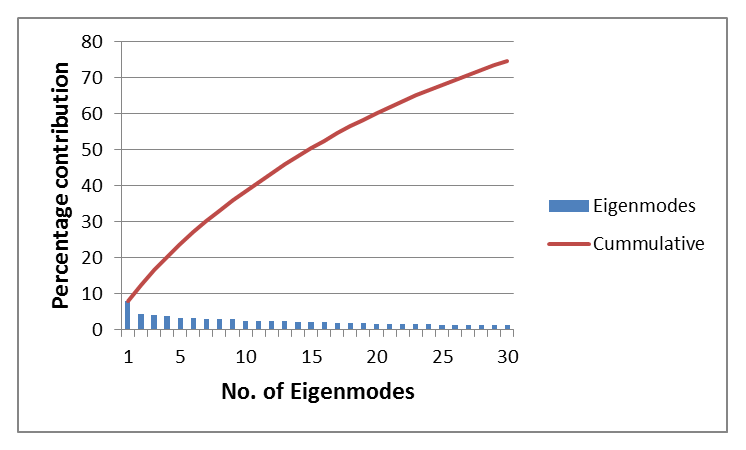
\epsfig{file = lh_CPNS_Eigen30.eps, width = 8cm}    
  \caption[Mean modes of variation for the cortex.]{Mean modes of variation for the cortical representation.}
  \label{fig:Modes}   
\end{figure}


The objective of using CPNS on the cortex is to detect cortical thickness variations.
In order to do this a test case is made using a base s-rep and 60 models derived from the same one.
The cortical thickness is reduced in specific regions of the cortex.
The datasets are created by adding some Gaussian noise to the position of the model, and to every spoke direction and radii in the s-rep. 
Each sample is going to be further modified with a linear variation of the cortical thickness,
specifically on the superior frontal and superior temporal regions of the cortex.
Spoke lengths are reduced $30\%$ of their original length.
If CPNS produces modes of variation, then the first mode should be related to the cortical thickness reduction.

Figure \ref{fig:Modes} shows the plot of the eigenvalues describing the mean modes of variation computed with CPNS.
The first mode is responsible for the largest variation found in the dataset and should correspond to 
thickness reduction in the specific areas. 

Figure \ref{fig:EigenVariation} shows the evolution of the model by manipulating the first mode of
variation. In the figure, the regions of the superior frontal
and superior temporal of the cortex are thinner, and adjacent structures remain constant through the deformation.
This can also be verified by checking the average thickness as shown in figure \ref{fig:thickness}.
As expected the first mode corresponds to the cortical thickness variation.

\begin{figure*}  
  \centering
  \subfigure[$+1.5 \sqrt{\lambda_1}$]{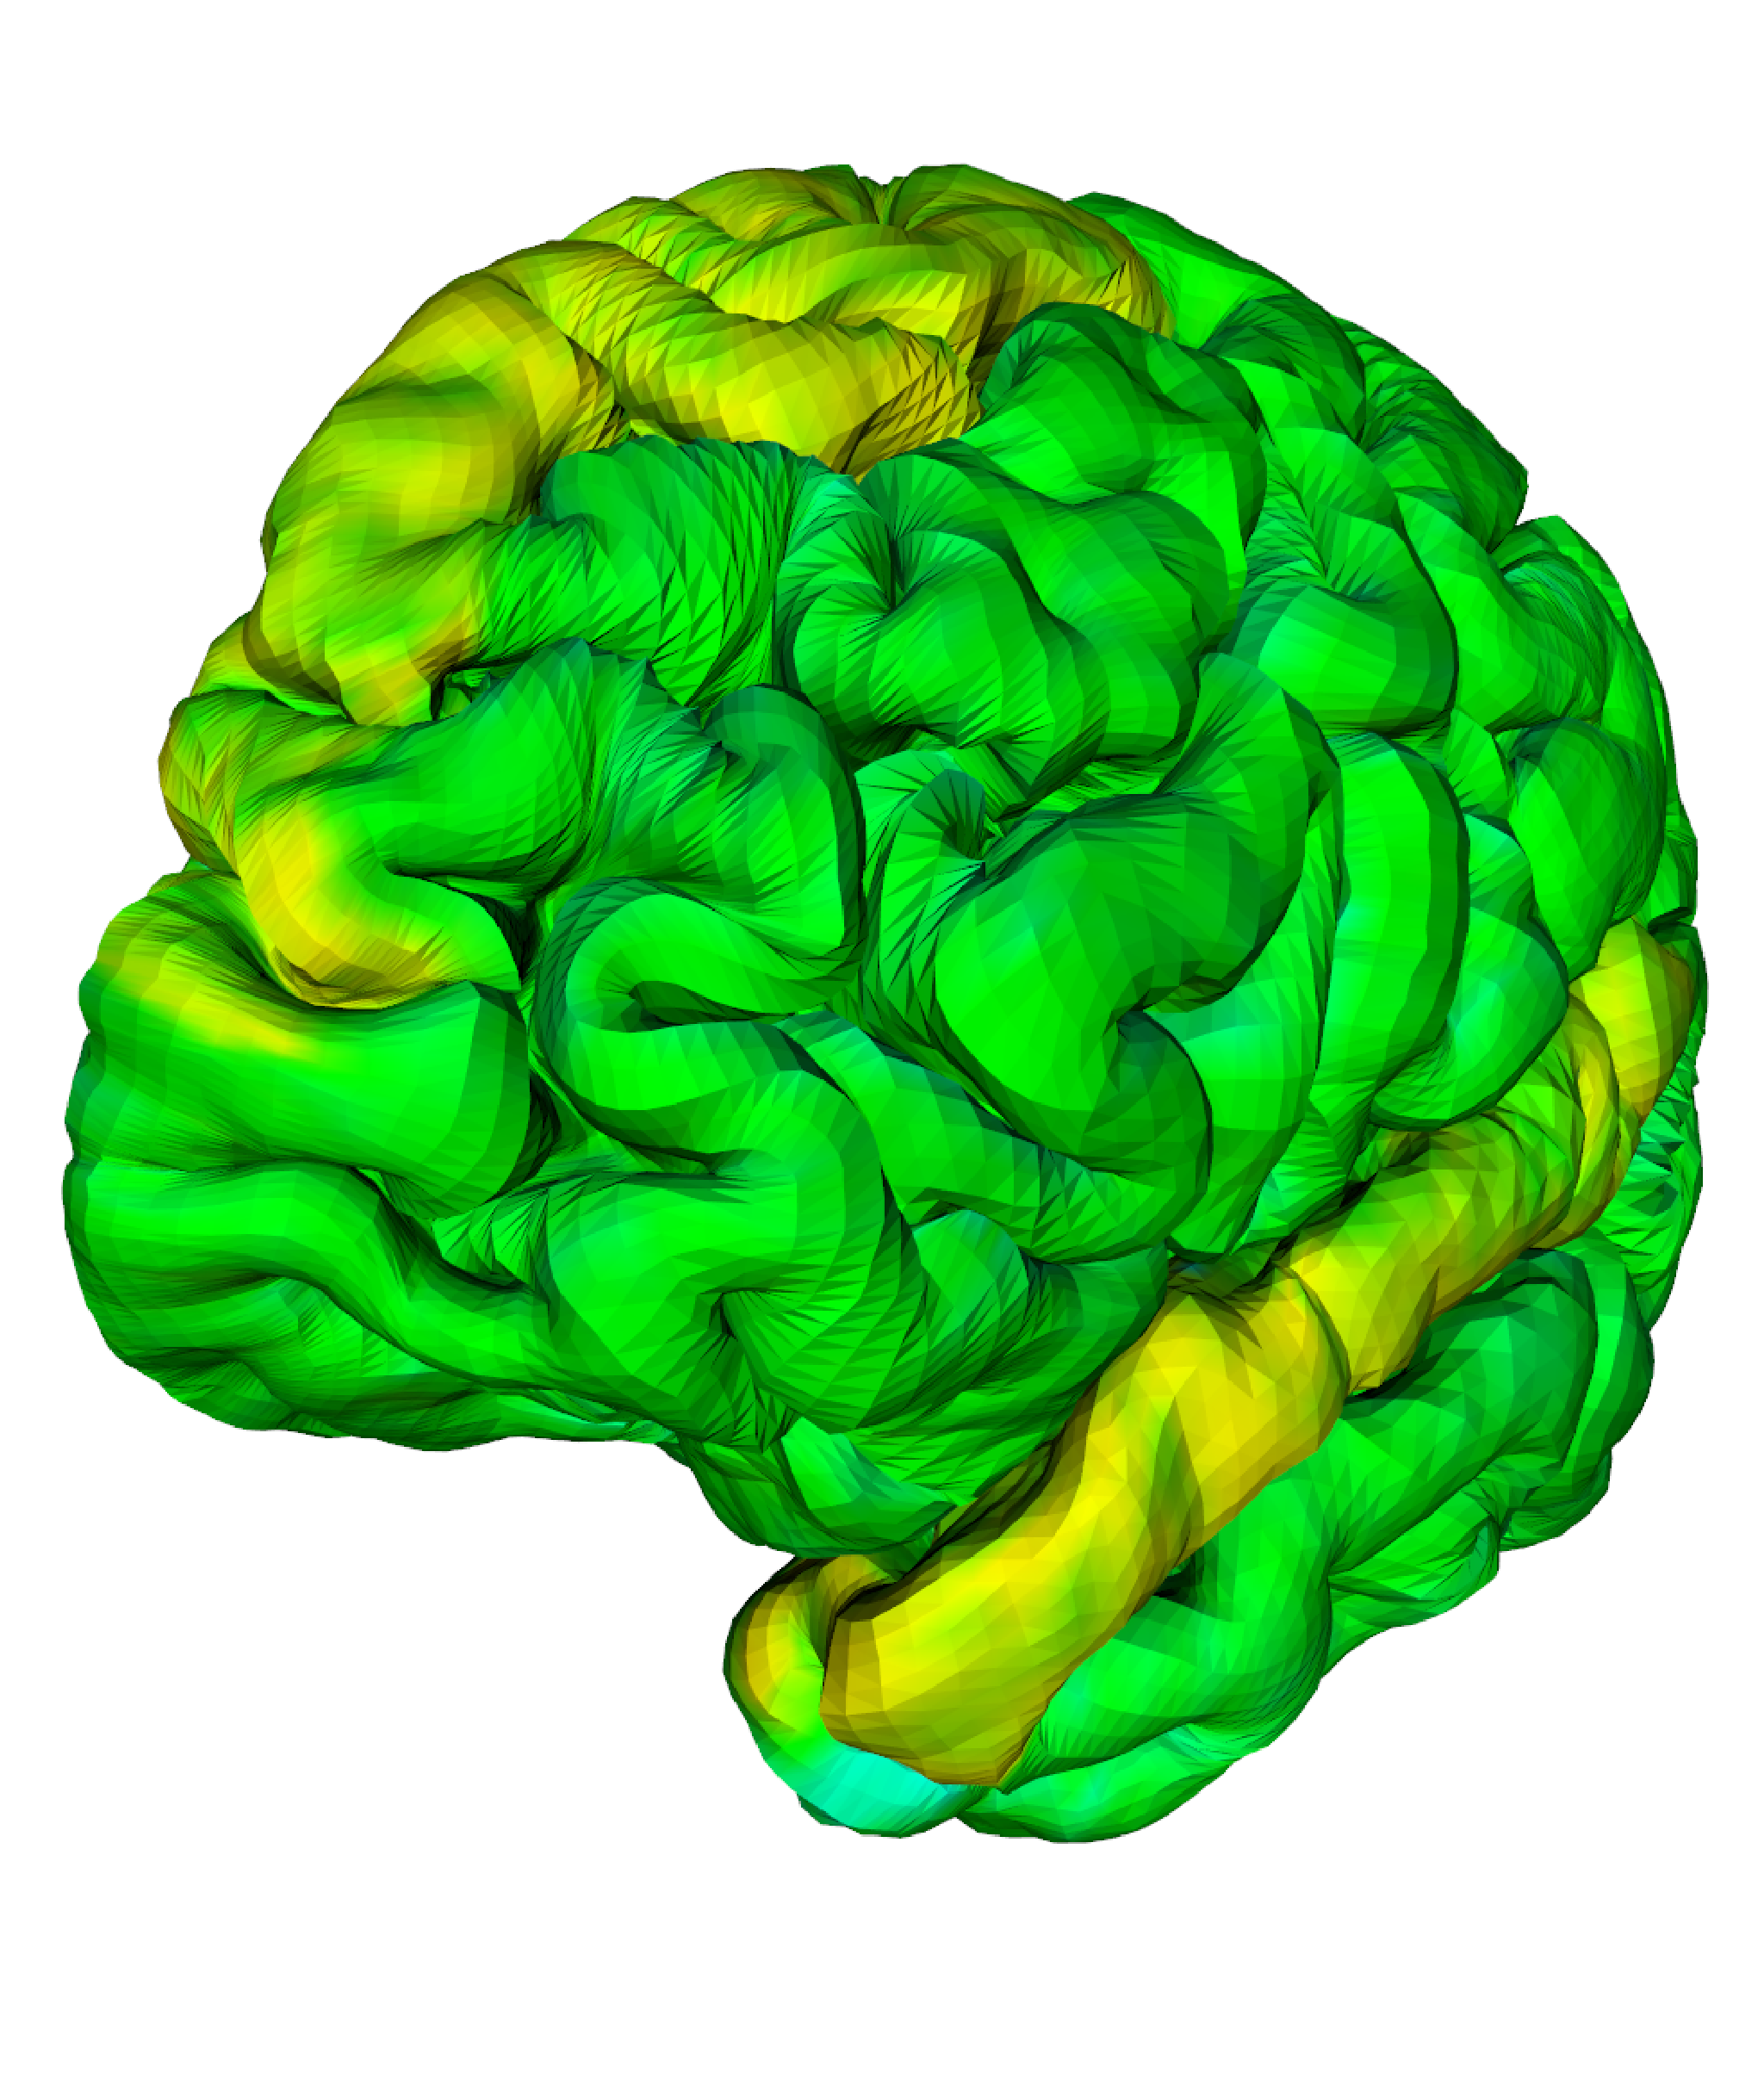
\epsfig{file = lh_EigenVariation30+1.5.eps, width = 3.5cm}}
  \subfigure[$+1  \sqrt{\lambda_1}$]{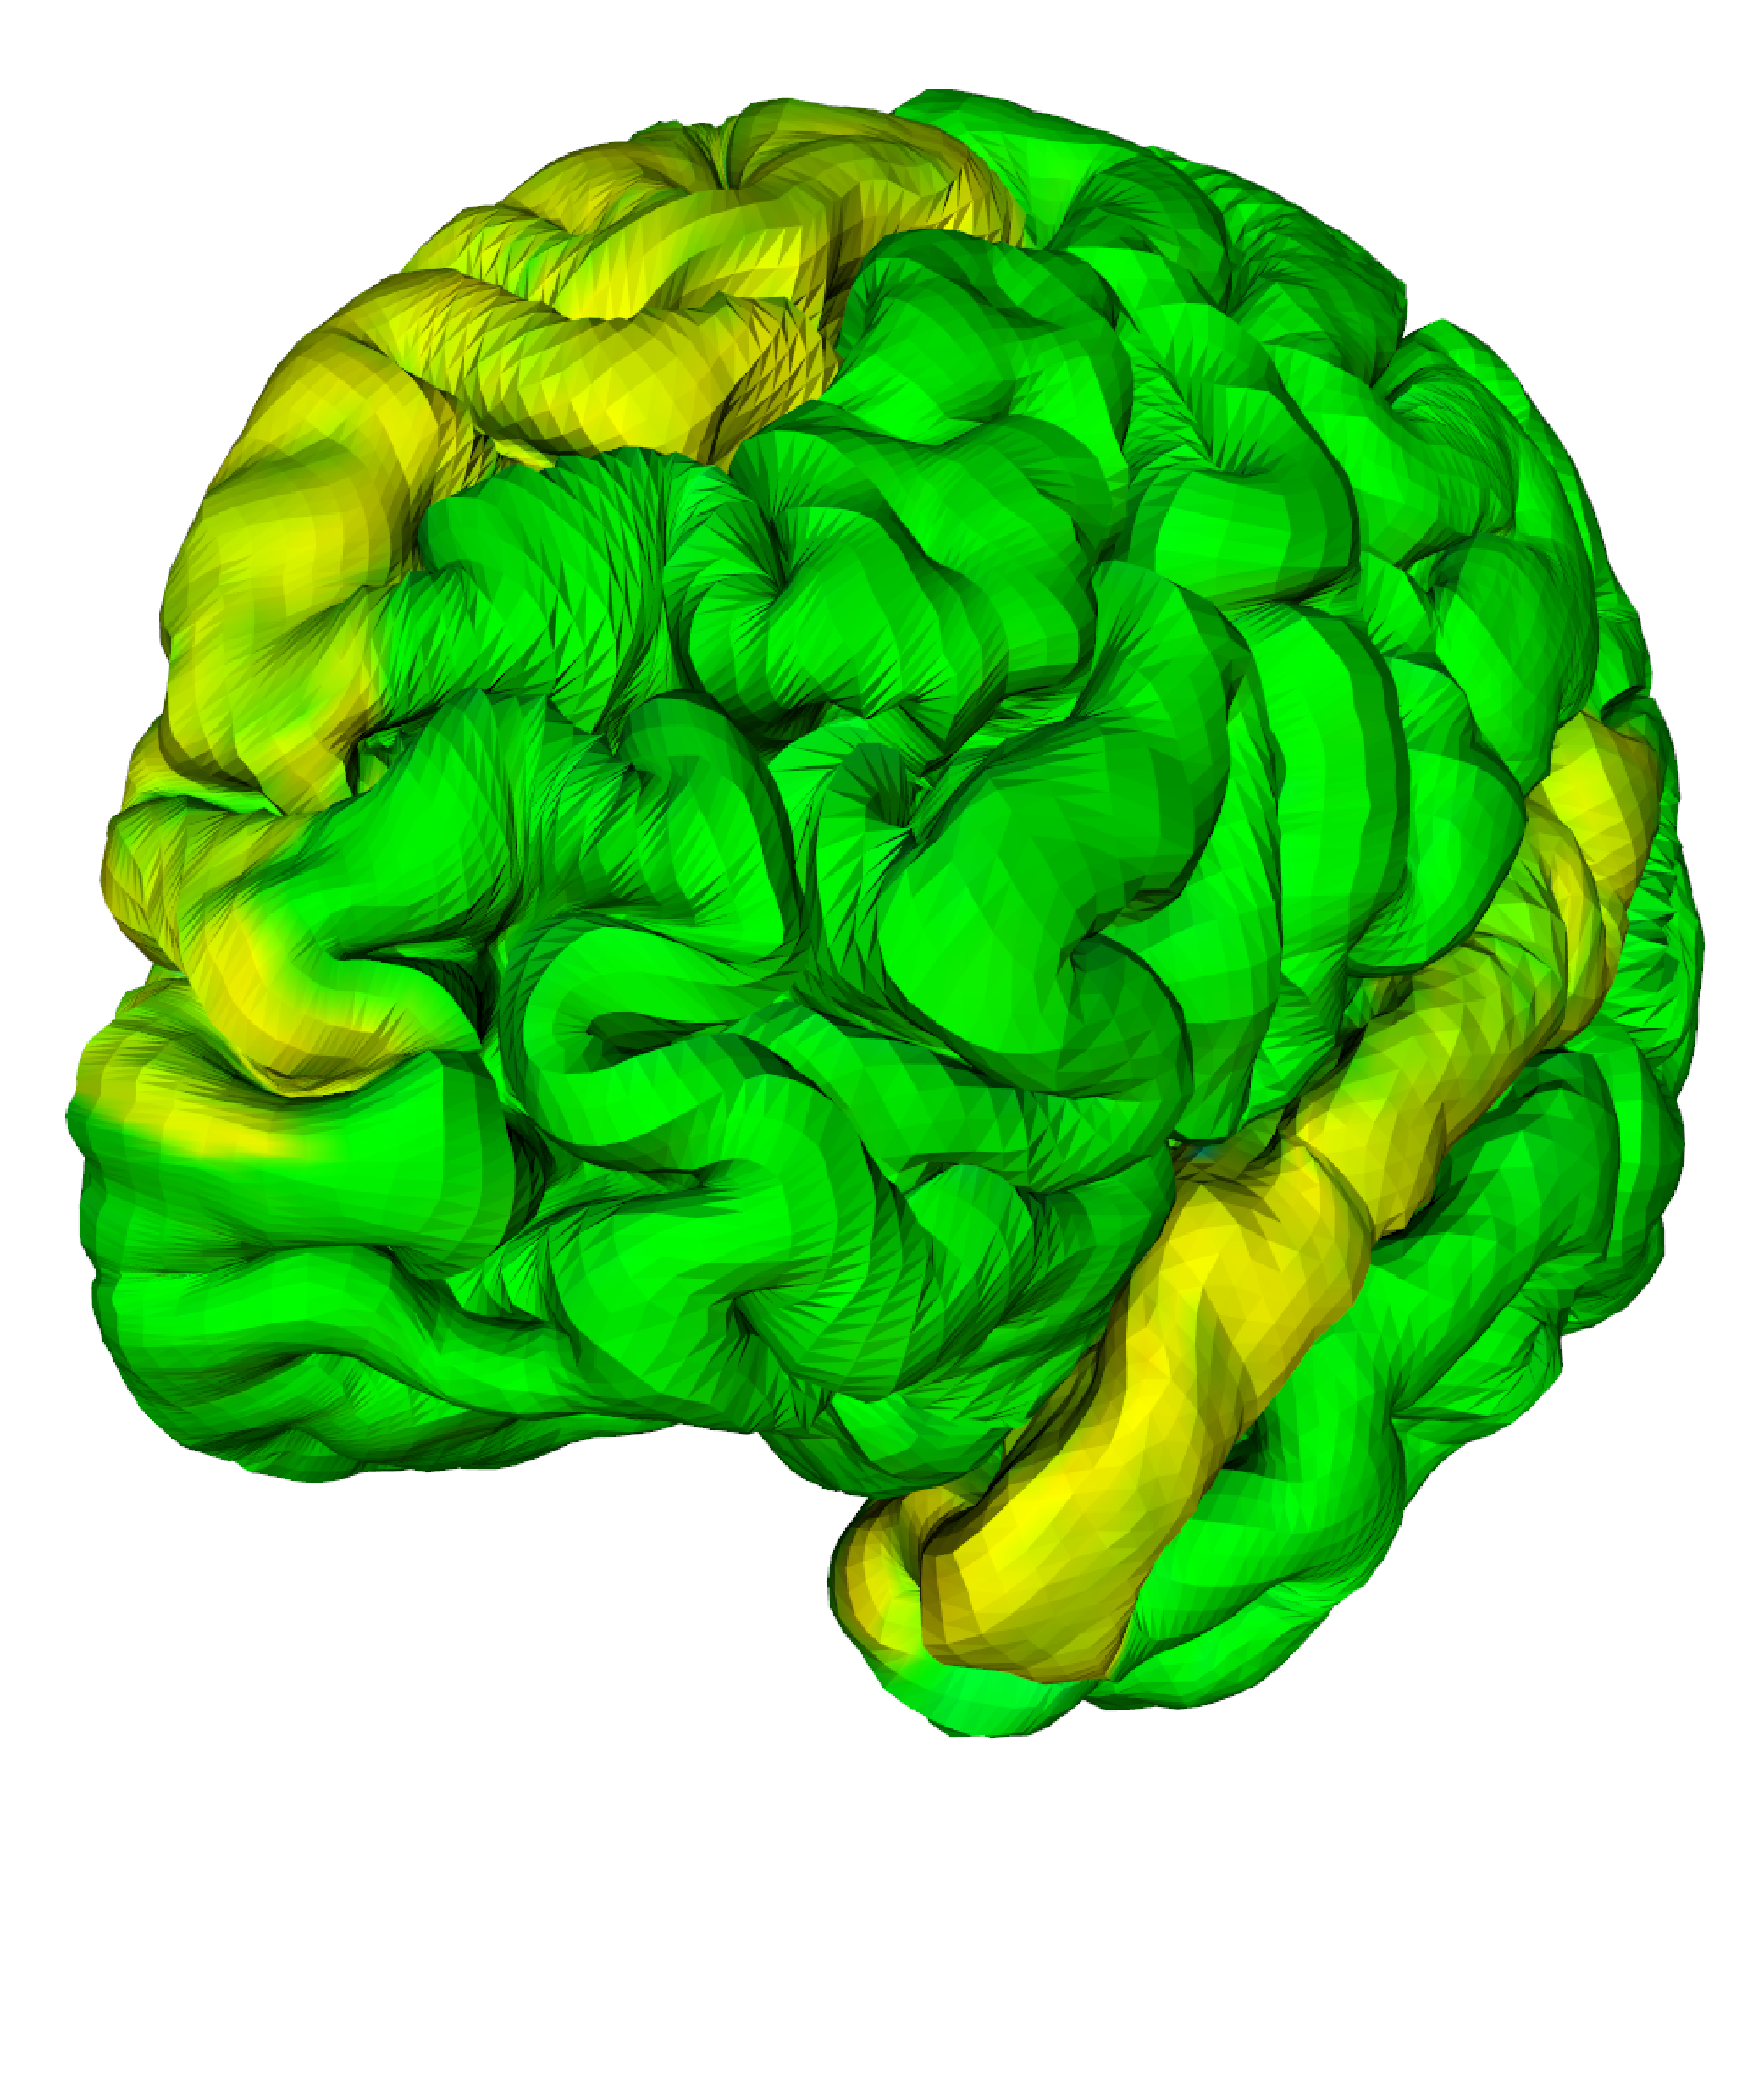
\epsfig{file = lh_EigenVariation30+1.eps, width = 3.5cm}}
  \subfigure[$+0.5 \sqrt{\lambda_1}$]{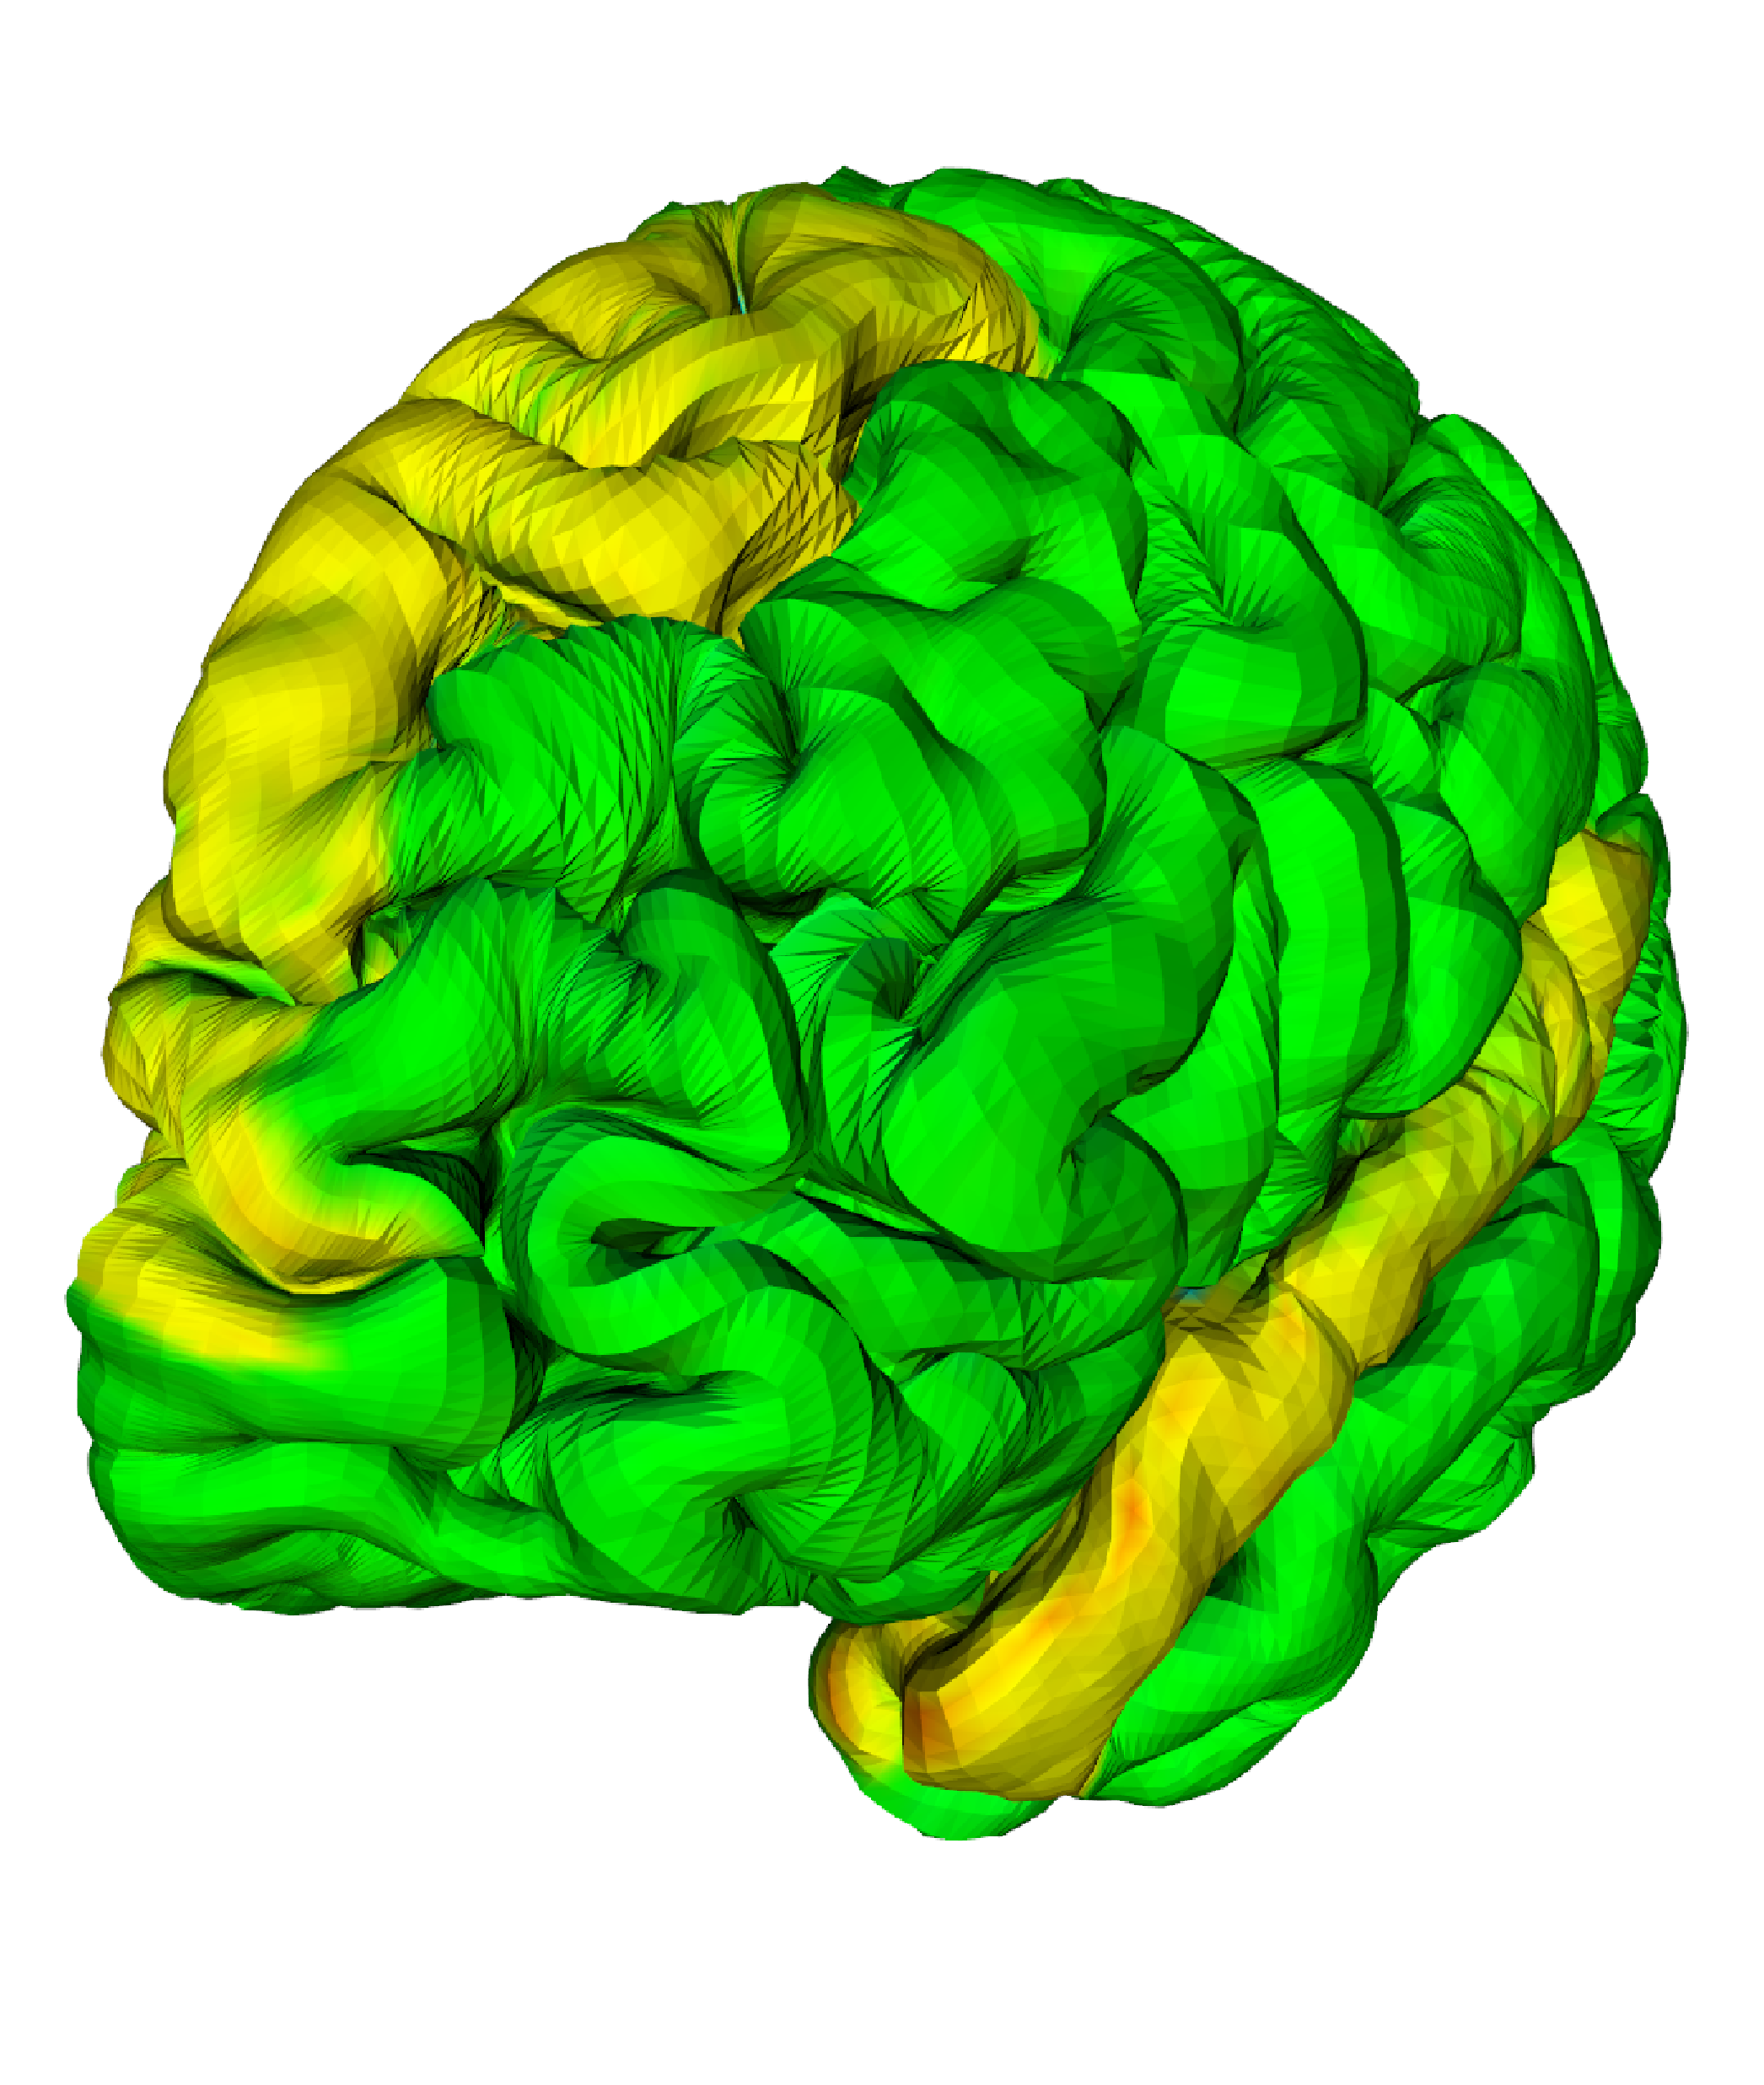
\epsfig{file = lh_EigenVariation30+0.5.eps, width = 3.5cm}}
  \subfigure[Mean]{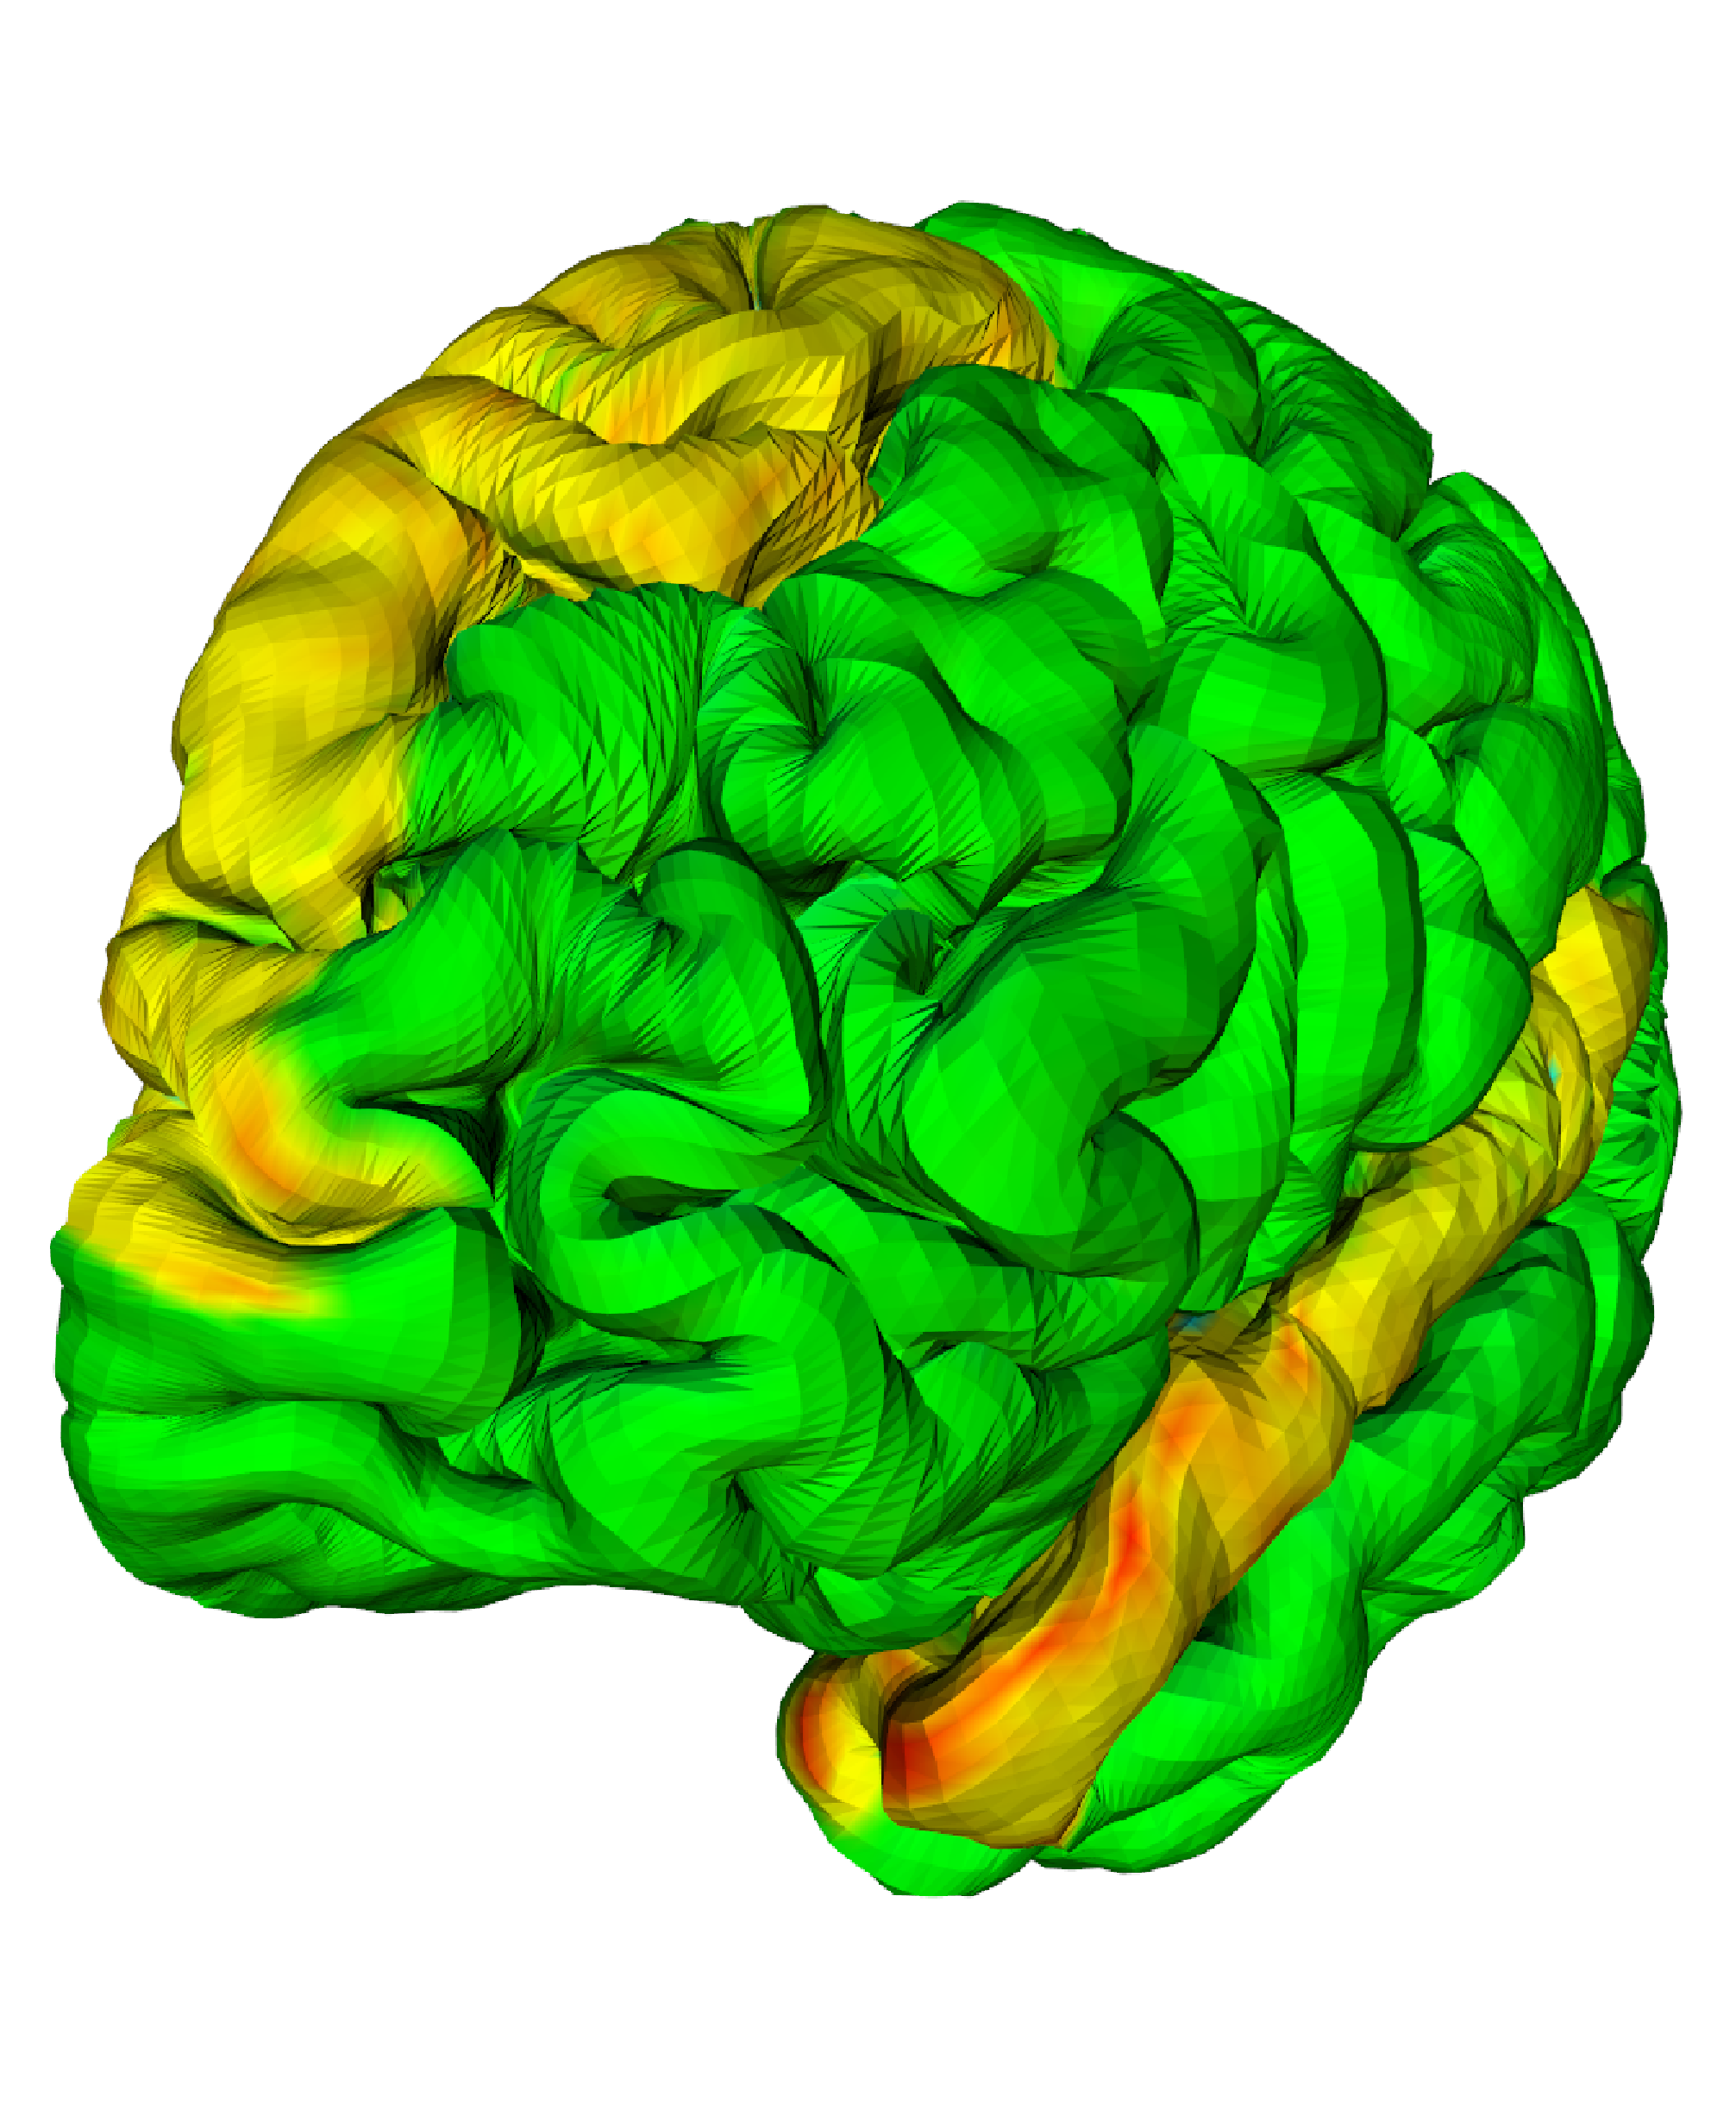
\epsfig{file = lh_EigenVariation30+0.eps, width = 3.5cm}}
  \subfigure[$-0.5 \sqrt{\lambda_1}$]{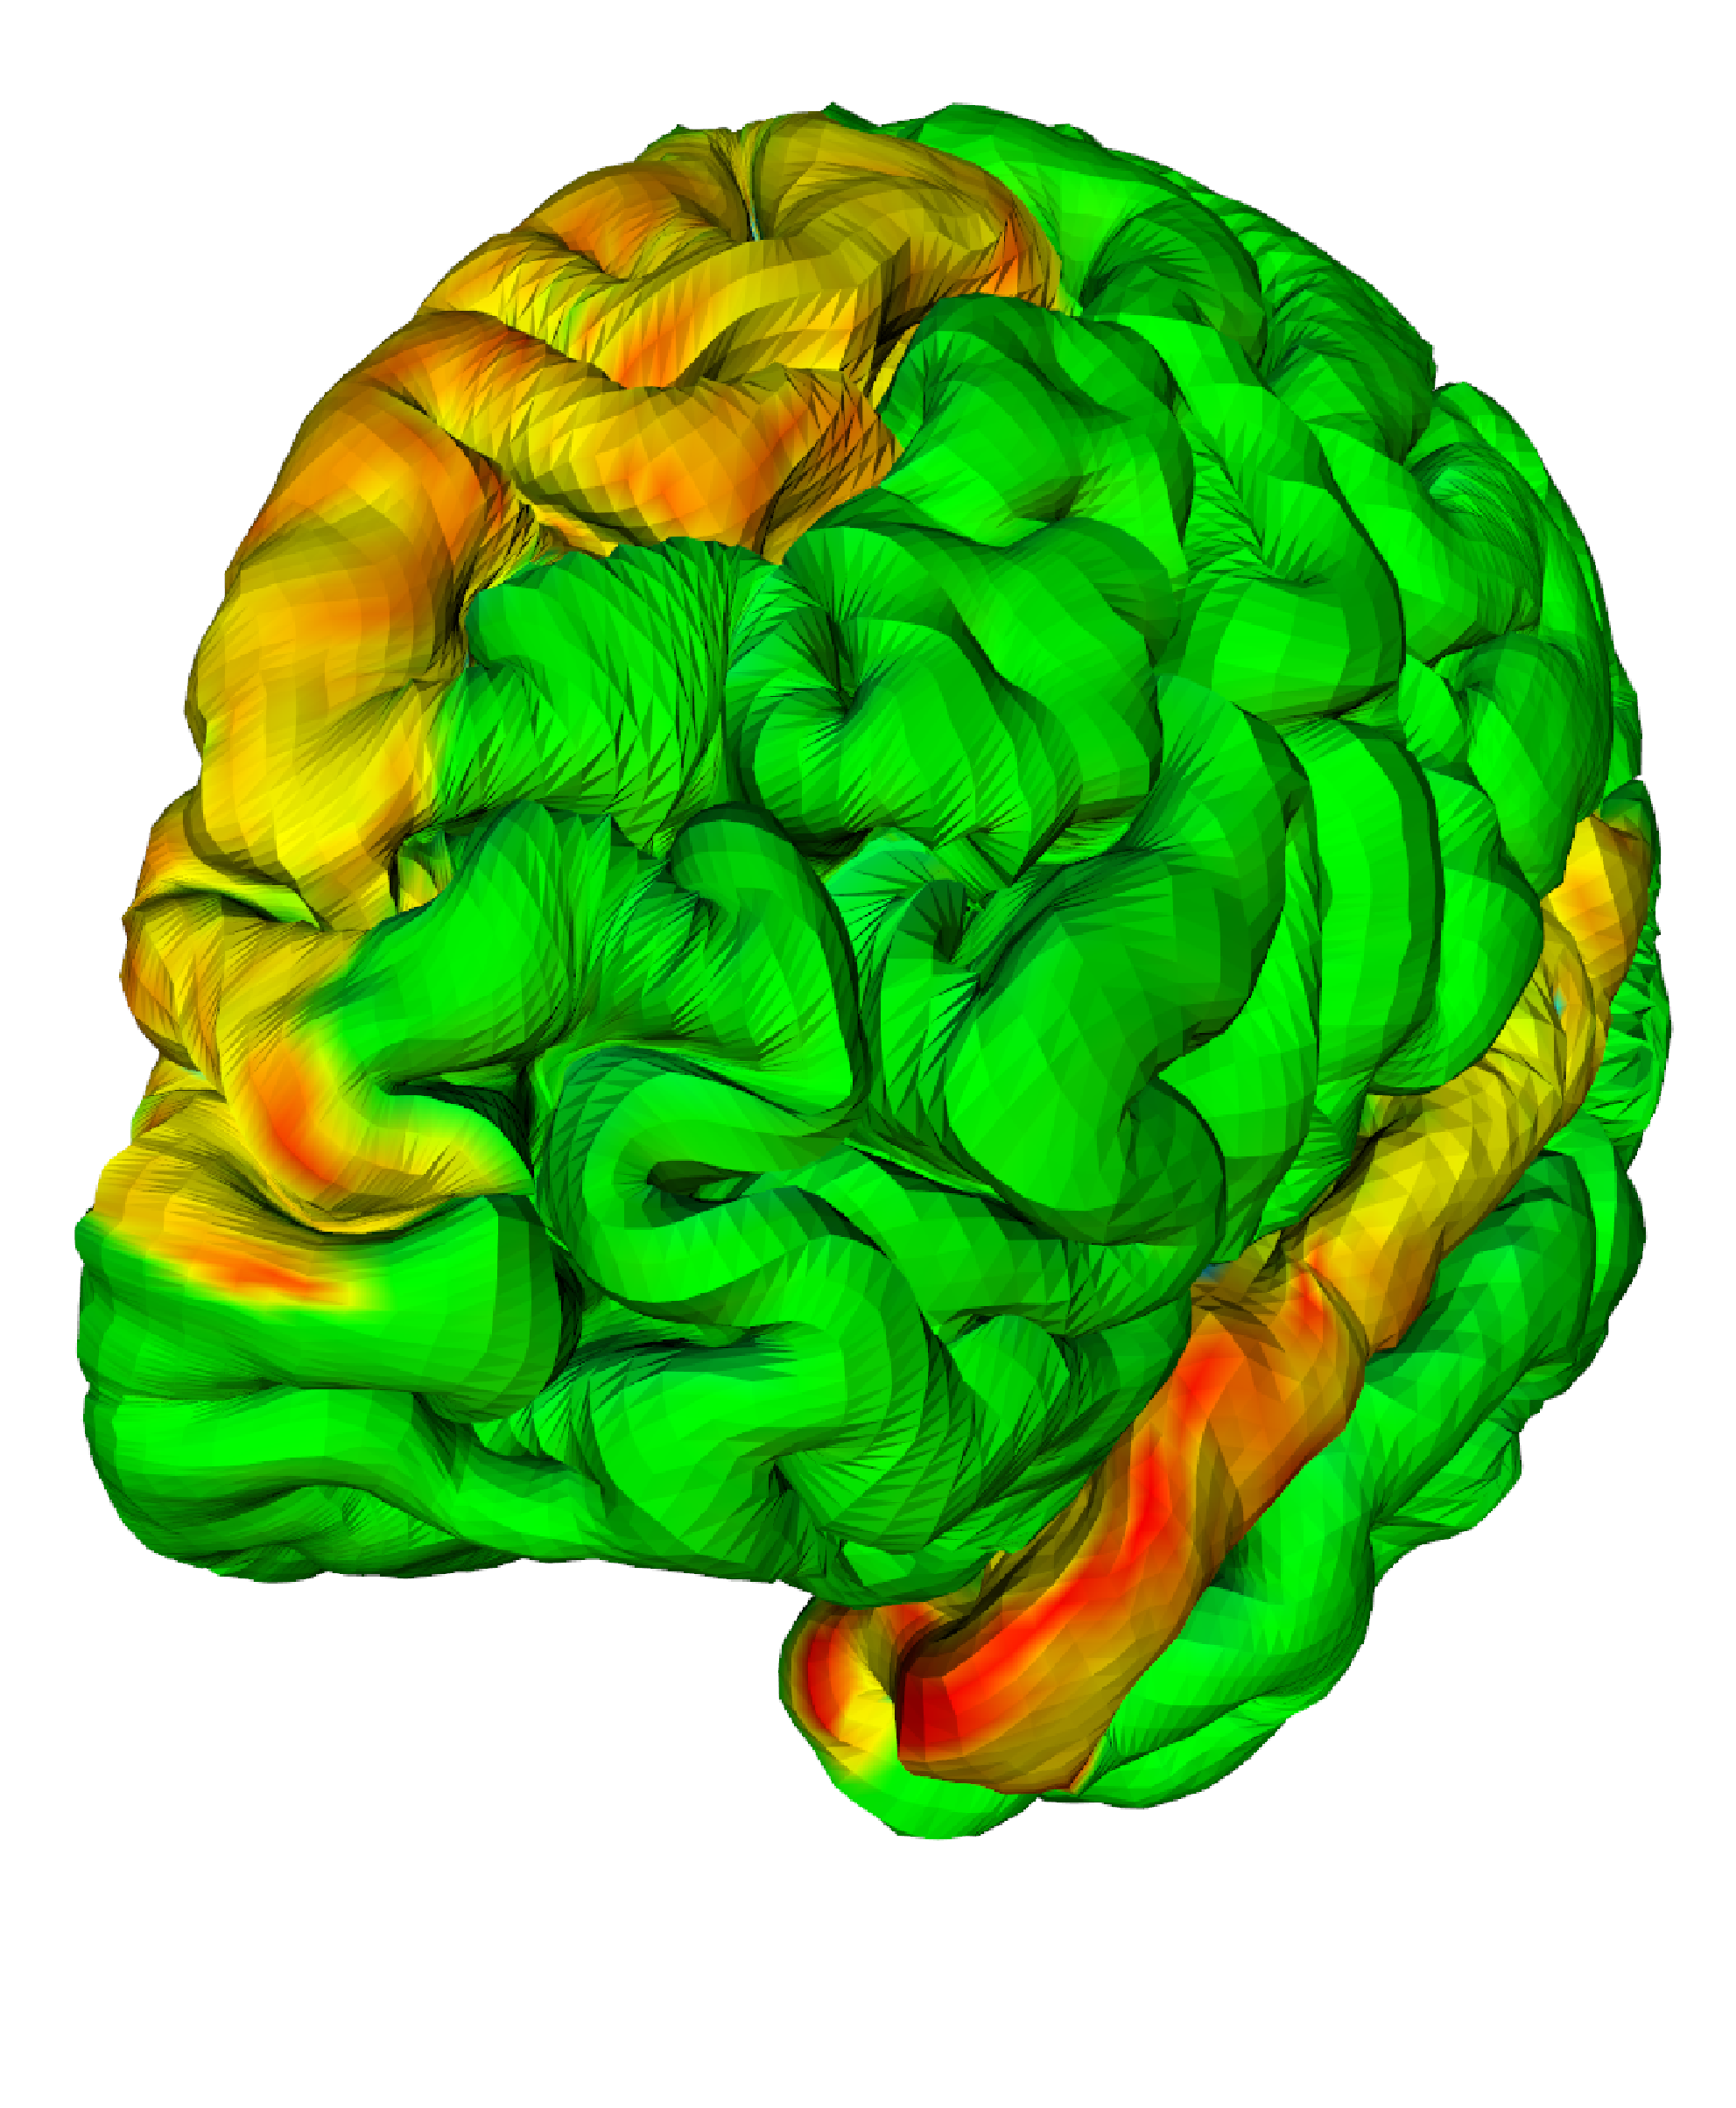
\epsfig{file = lh_EigenVariation30-0.5.eps, width = 3.5cm}}
  \subfigure[$-1 \sqrt{\lambda_1}$]{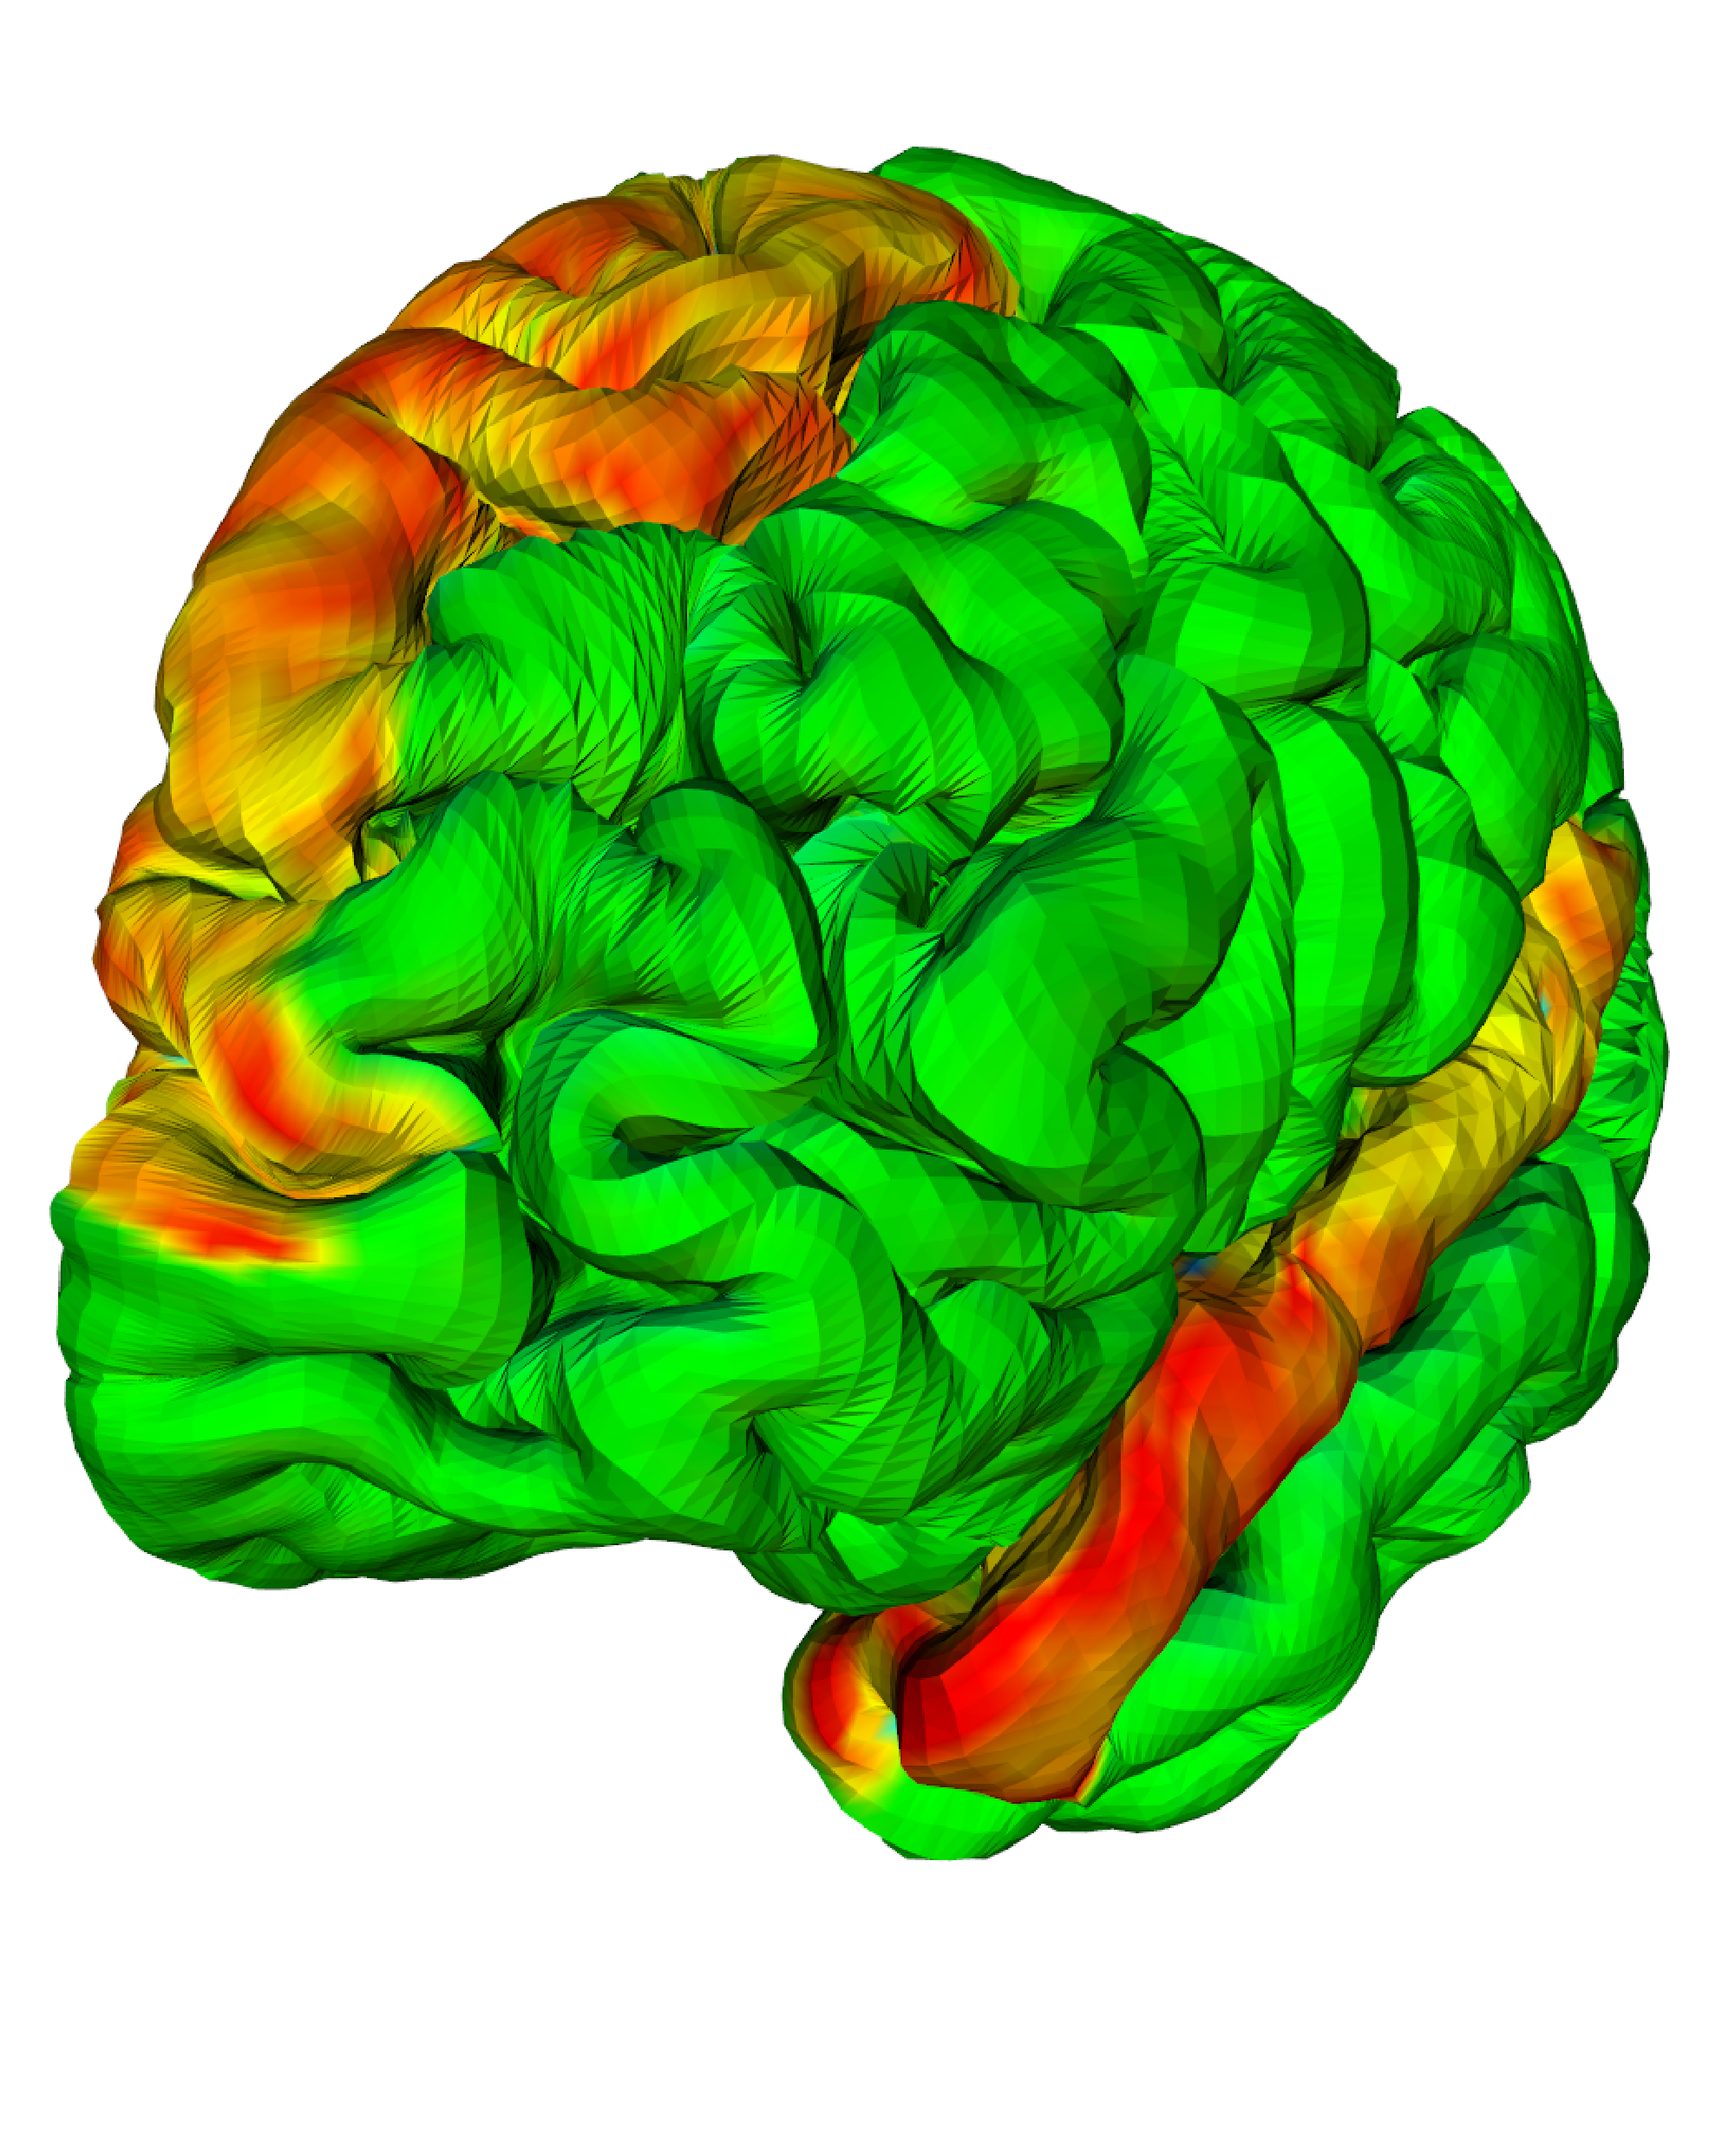
\epsfig{file = lh_EigenVariation30-1.eps, width = 3.5cm}}
  \subfigure[$+1.5 \sqrt{\lambda_1}$]{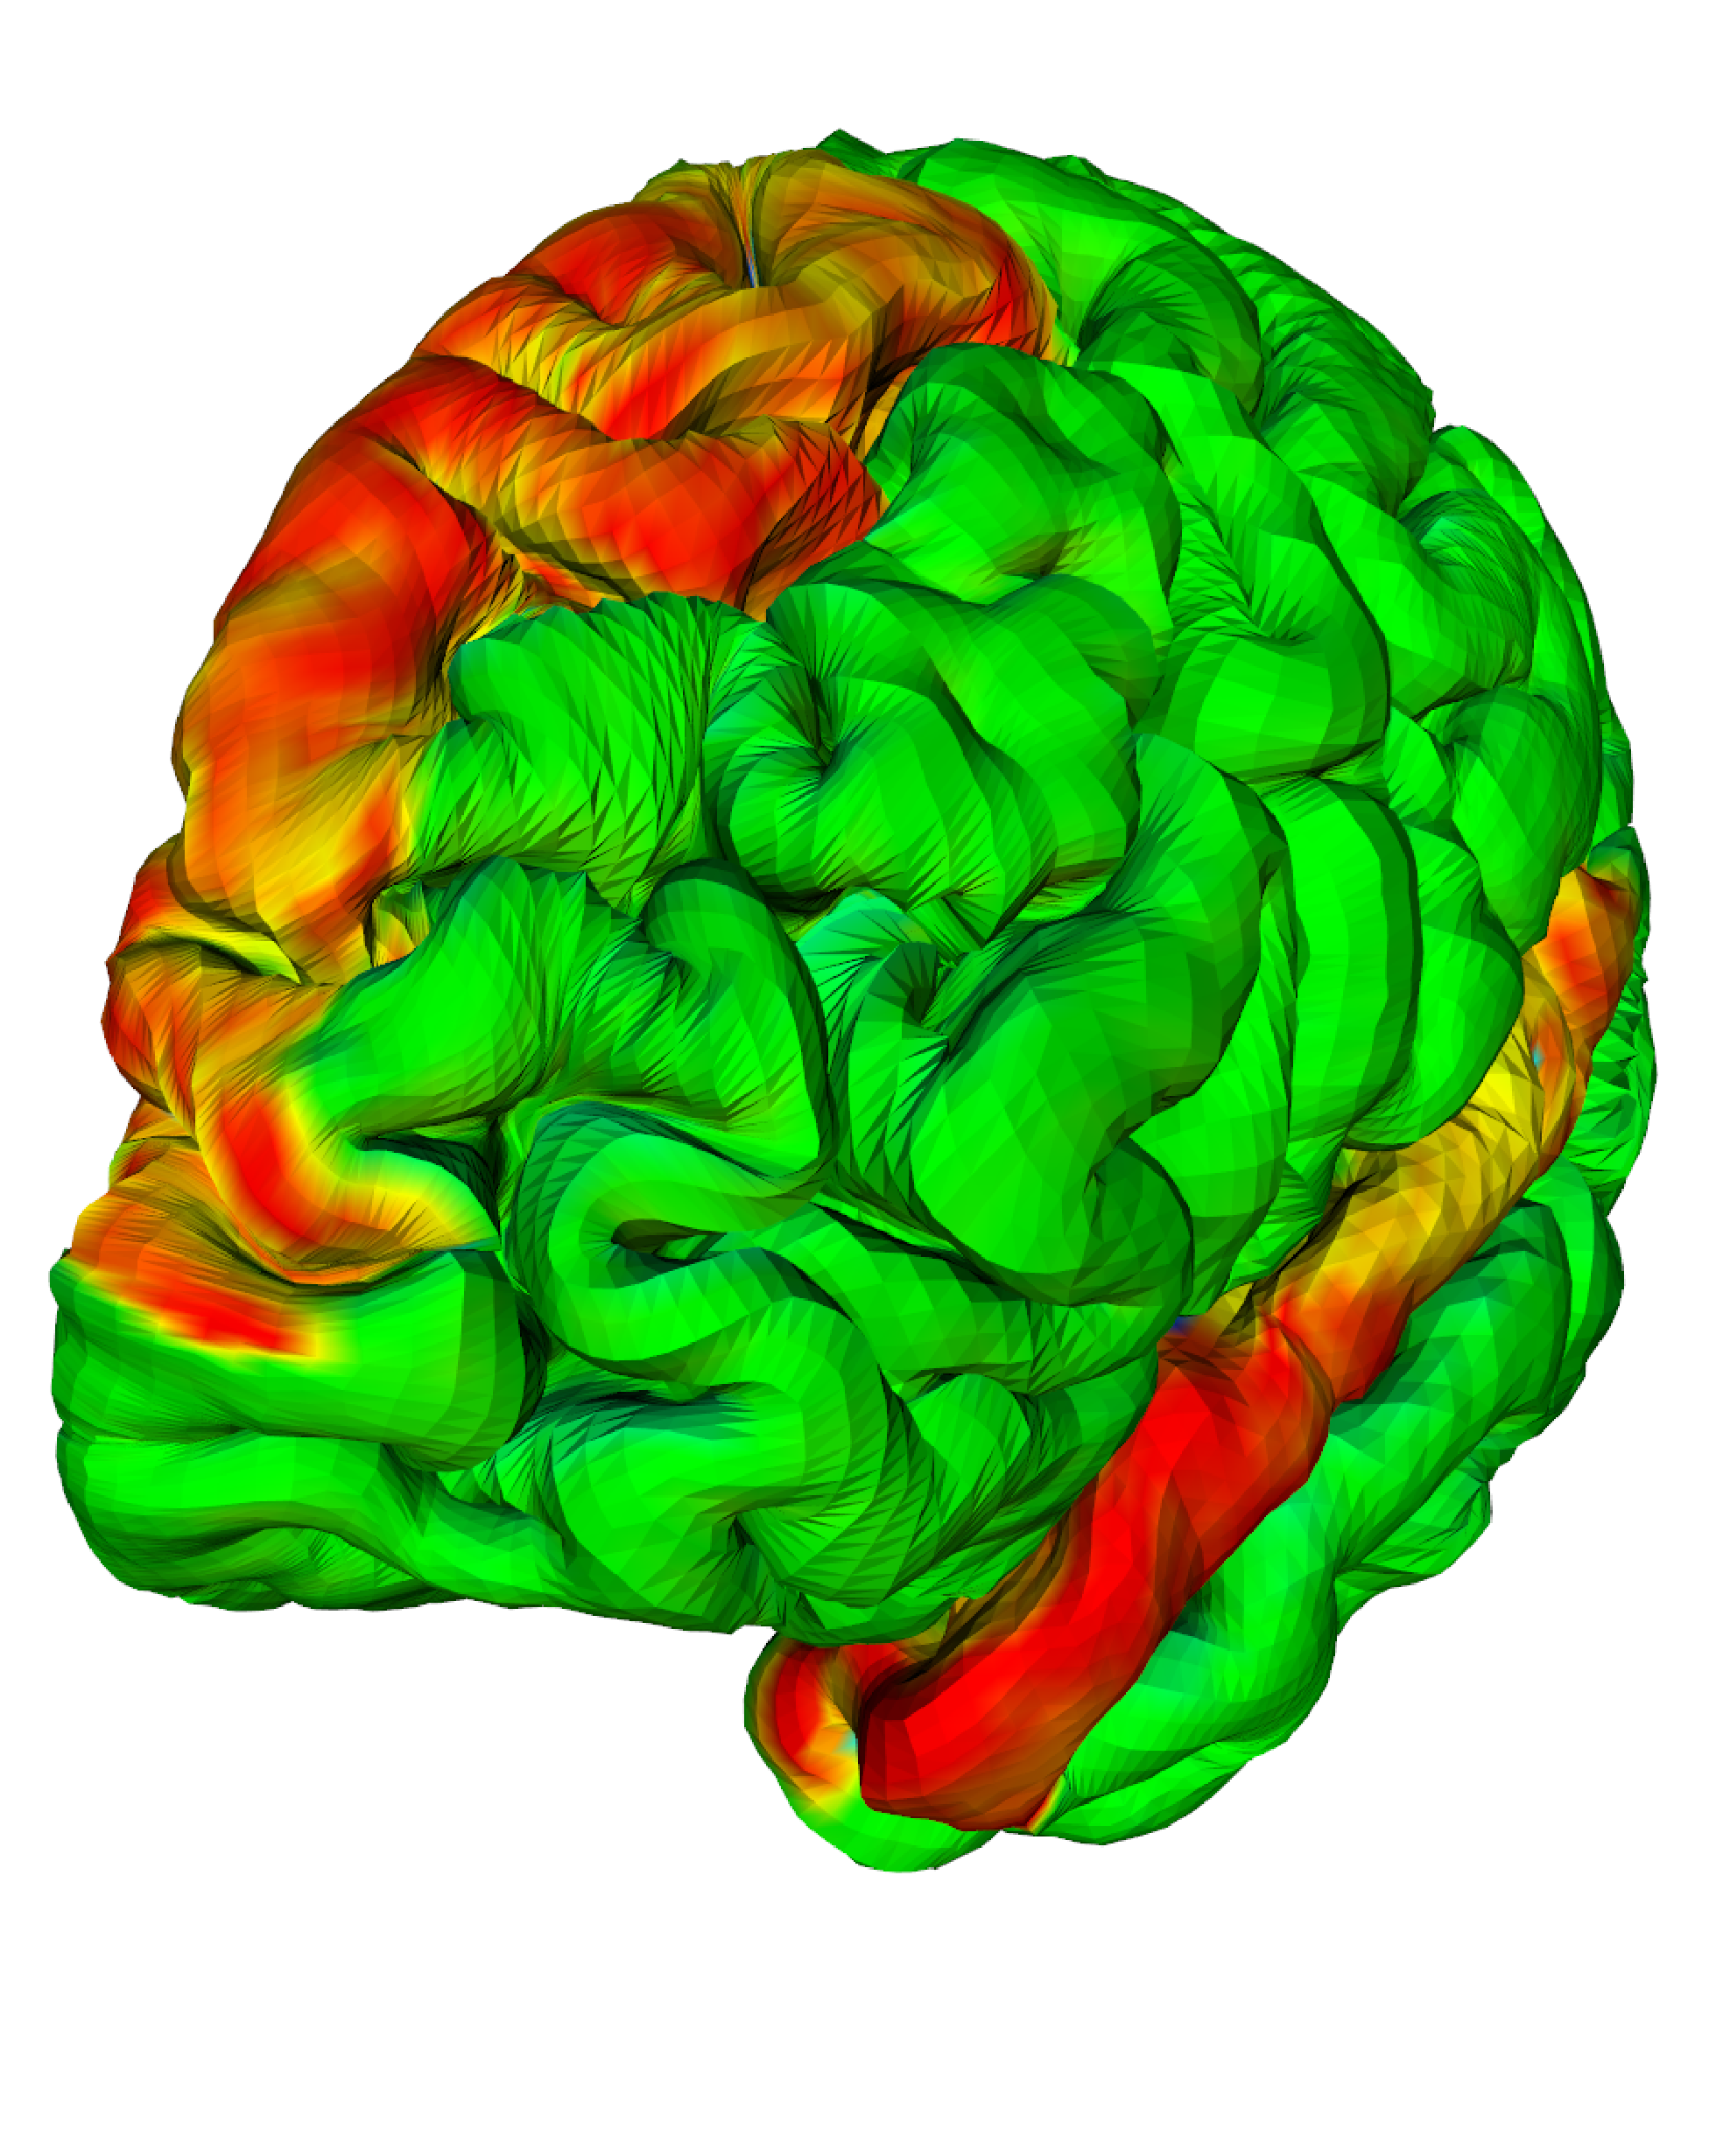
\epsfig{file = lh_EigenVariation30-1.5.eps, width = 3.5cm}}
  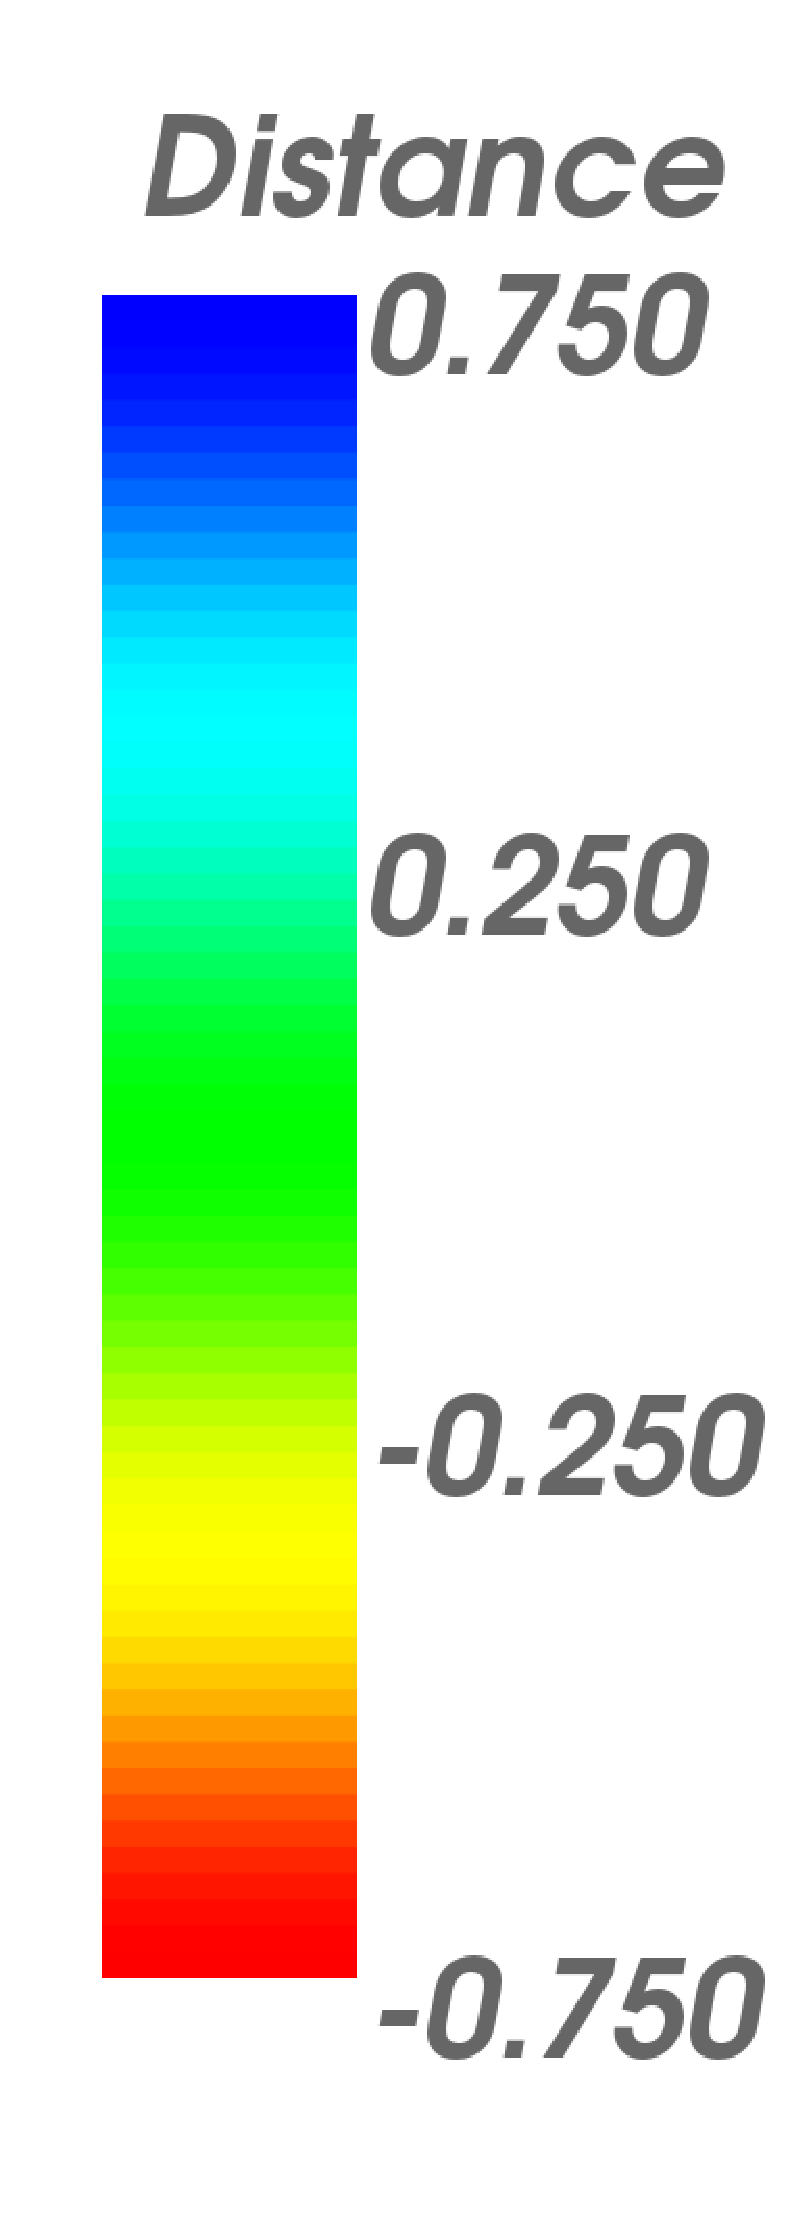
\epsfig{file = lh_EigenVariation30Bar.eps, width = 1.75cm}
  \caption[S-rep deformation using the first mode.]{Deforming the s-rep model using the first mode of variation and comparing it against the base s-rep.}
  \label{fig:EigenVariation}   
\end{figure*}

\begin{figure}[htb] 
  \centering
  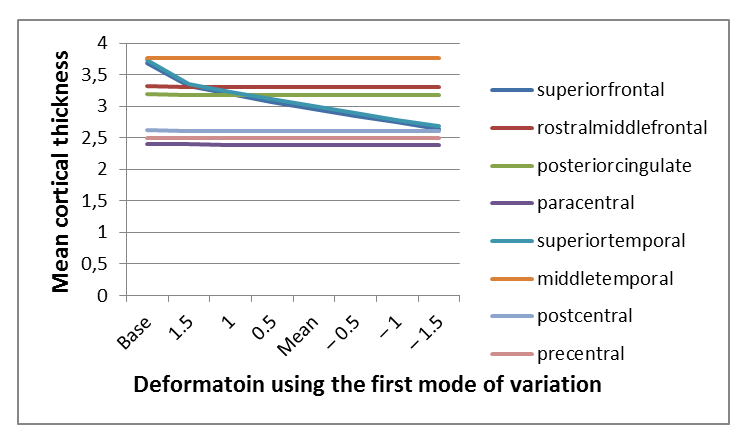
\epsfig{file = lh_EigenVariation.eps, width = 9cm}    
  \caption[Average thickness of the cortex.]{Average thickness for some cortical regions in the cortex. The two regions changing through the deformation
           are the superiorfrontal and superiortemporal.}
  \label{fig:thickness}   
\end{figure}


\section{Conclusion}
\label{sec:Conclusion}

One of the major contributions of this work is to represent the cortex as a folded slab using s-reps. 
S-reps are able to model continuum space. This characteristic can be used 
for the following purposes:
to include information in the cortex at different scale levels; provide 
new ways to analyze cortical columns, the building blocks of the cortical tissue;
analyze cortical lesions in a different space. 

These new advantages will use the local coordinate system $[u,v,\tau]$ provided by s-reps. 

A second contribution is to provide a compact representation of the cortex using CPNS. 
This statistical description models cortical thickness variations with a mean shape, some eigenmodes and a few coefficients.
Previous work with CPNS was done to study shape variations on the hippocampus using a grid size of $8*3$ atoms 
to represent the population of objects.
In this case, the s-rep size is $160 \times 160 $ atoms; nevertheless, CPNS was able to capture the localized thickness variation produced 
in the superior-frontal and superior-temporal regions of the cortex. 
This suggests that the approach could
produce statistics for longitudinal clinical 
cases that are characterized by cortical thickness variations. 
Cortical thinning is a natural process of aging \cite{doi:10.1080/13803390802635174}.
Other clinical cases such as psychosis, schizophrenia, hyperactivity disorder in children and autism
also present abnormal cortical thickness variations.

A third contribution is to model the cortex of different patients using the same underlying skeletal structure.
A test case was done to compute a mean shape of the cortex for the 8 patients used in this study. 
%This characteristic could be exploited if the statisitcs are computed for a crosswise scenario.
%Any approach that computes shape statistics, must have 
%a stable set of points or landmarks across the population and this is achieved using the SS of the s-rep.
Figure \ref{fig:CPNSMean} shows the mean surface for the 8 datasets computed with \textit{Freesurfer} and
CPNS. 
%To compute CPNS with the 8 subjects used in this study, 
%the cortical regions mapped on the sphere 
%are aligned to a generic template. 
%Using the aligned spheres to generate the s-reps
%increases the correspondence of the SS accross the population. 
%Each hub of the s-rep should map to the same region 
%in the cortex in order to perform an accurate 
%statistical analysis of shape with CPNS. 

Unfortunately in this case, CPNS was not able to detect principal modes of variation.
%and yield the set of eigenmodes unusable.
This could be for two reasons. The main one is related to the number of datasets 
used in the study. The dimension of the s-rep 
is too high compared to the sample size.
The second reason could be related to the alignment 
of each of the cortical regions. 
To produce accurate shape statistics, the objects must be aligned correctly.


\begin{figure}  
  \centering
  \subfigure[CPNS mean]{\epsfig{file = cortexCompareCPNS.eps, width = 7.25cm}}
  \subfigure[\textit{Freesurfer} mean]{\epsfig{file = cortexCompareFreesurfer.eps, width = 7.25cm}}
  \subfigure[Overlap]{\epsfig{file = cortexCompareOverlap.eps, width = 8.5cm}}  
  \caption[Mean shape of the cortex: CPNS and \textit{Freesurfer}.]{Mean shape computed from the 8 datasets.}
  \label{fig:CPNSMean}   
\end{figure}

It has been proven that s-reps are suitable 
entities to model the complex shape of the cortex and provide new ways of cortex analysis. 

Future work considers the following possibilities:
the first opportunity is related to shape analysis of the cortex in 
multiple subjects scenarios. The objective is to produce a usable set of coefficients
and eigenmodes that models a population of cortices.
A second opportunity is related to cortex analysis on longitudinal scenarios. 
For this purpose three or more acquisitions of a patient at different time points could be used 
to study the process of aging. 

The work presented here showed that CPNS can detect cortical thinning on a set of cortices; 
a third line of work seeks to describe the folding procedure of the cerebral cortex
using shape descriptors.

The following chapter explains a texture synthesis technique to create volumetric representations using 
2D image samples. The volumes can be used on s-rep models to create 
solid objects.


\newpage


\input{ChapterTexture/ChapterTexture}
\input{ChapterSimulation/ChapterSimulation}
\chapter{Conclusions and perspectives}
%\addcontentsline{toc}{part}{Conclusions and perspectives}
\label{chapter:Conclusions}

\section{Synopsis of the work}

The principal objective of this dissertation was to propose a technique able 
to model internal and external features of organs. 
Describing internal features and 
surface characteristics closes the gap 
between virtual objects and objects in the real world. 
Objects with such characteristics are needed to improve 
existent simulation procedures. 

After reviewing the state of the art techniques for 
shape modeling, it can be concluded that 
s-reps provide features superior to other techniques. 
One of the most important characteristic of this technique
is the possibility to describe the interior of an object. 
This quality was widely used through this dissertation.
It allows including information from different spatial scales
or sources such as histology images and/or physical parameters. 

To prove the capabilities of s-reps, 
the human brain became the target organ to be modeled.
From this task came the 
most important contribution of this dissertation,
which is the procedure to model the 
cerebral cortex using s-reps. 

The cerebral cortex has never been modeled 
with techniques describing internal features. 
From now on, a single non-branching object 
can be used to describe both cortical surfaces plus the interior. 
S-reps provide new ways to analyze cortical columns and analyze cortical lesions in a different parametric space.

Besides describing the shape of the cortex, it was proven 
that a population of cortices can be described by a mean shape, a set of eigenmodes 
and some coefficients. CPNS and the cortex representation 
enabled a compact representation or a statistical description of thickness 
variations in the cortex. 

The second objective of this dissertation, \textit{i.e.}, 
to provide a mechanism to model the volumetric properties of an object,
was fulfilled with a method to synthesize solids. 
This technique is compatible with s-reps and 
allows describing the interior of the object using parameters from various sources such as: 
RGB textured images; images from histology; images from $\mu MR$ and $\mu CT$; and physical parameters. 

A simulation of the brain was done using 
the techniques just described. 
S-reps of the subcortical structures were fitted 
to real MRI images segmented with \textit{Freesurfer}.
The subcortical structures include: amygdala, caudate, hippocampus, lateral ventricles, pallidum and putamen.

Using this set of s-reps, 
the internal properties of the objects were enhanced 
with textures of physical parameters. 
MRI images were simulated using the virtual object and \textit{SimuBloch}. 
The MRIs were validated using the automatic segmentation 
procedure proposed by \textit{Freesurfer}.

\section{Future work}

There are three possibilities identified for future work.
Improvement of the statistical shape description of the cortex, 
improvement of the simulation framework
and working towards the establishment of a technique 
to estimate scalar features based on shape descriptions.

The shape description of the cortex 
with s-reps and CPNS could
provide new research opportunities to
analyze shape variability in control and pathological subjects for crosswise (multiple subjects)
and longitudinal (same subject but multiple acquisitions) scenarios.
The shape description of the cortex could help researchers understand 
brain development and to identify the principal shape variations as the human brain grows. 
%Enhancing current knowledge should lead to novel theories. 

The simulation framework can be improved 
by acquiring better textured samples of physical parameters 
and generating statistical shape descriptions of the organ structures 
modeled with s-reps.

As mentioned in Section \ref{sec:ConclusionsSimu} the full potential of 
the approach to simulate images is not achieved. The textured samples 
do not contain structural information and they have a low resolution. 

With the statistical shape descriptions of organs, 
a completely different set of structures can be generated
using a few coefficients.
Control and pathological shapes can be combined to produce new simulated images.

There are two major applications for this framework, 
the optimization of image acquisition parameters 
and the validation of segmentation algorithms.

Finally, 
a methodology to estimate scalar features based on shape description needs to 
be established. 
For example, we wish to estimate the gray matter anisotropies
in thalamic nuclei based on a fitted s-rep to the structure
and clinical resolution DTI images. 

The nuclei are only visible in a high resolution DTI acquisition. 
Unfortunately, this acquisition cannot be done routinely.
In order to identify this feature, 
a set of patients with DTI and $T1-$weighted image
acquisitions will be used in the study. 

The procedure will use the $T1-$weighted images to fit s-reps.
The fitting produces tight representations of an s-rep
and increases the correspondence between internal positions $[u, v, \tau]$ among thalami.

Shape statistics will be computed using CPNS, 
and a statistical analysis will be done for 
the nuclei density using the coordinate system $[u, v, \tau]$. 
This is possible since the internal positions are in correspondence.

The statistics will contain shape and nuclei density 
descriptions for each position inside the s-rep. 

To estimate the nuclei density in a new thalamus, 
the mean shape produced by CPNS is fitted to the structure.
The nuclei density can be estimated based on 
the shape deformation and the density statistical description. 

This approach could be use to detect other type of scalar features. 

\chapter{Résumé de thèse}
\label{chapter:IntroductionFR}

\section{Introduction}

Les progrès récents sur les modalités d'imagerie et de calcul numériques ont ouvert un nouveau 
domaine d'étude de la variabilité biologique de l'anatomie humaine. Ce nouveau domaine est appelé 
l'\textit{anatomie computationnelle} (CA).

La CA, telle que définie par \cite{Grenander1998}, possède trois aspects principaux : construction de formes 
anatomiques ou modélisation par des points, des courbes, des surfaces et des volumes ; comparaison de ces modèles ; 
et l'analyse statistique de la variabilité de forme.
Les statistiques permettent de déduire et de tester des hypothèses d'états pathologiques. 
Cela se fait à l'aide de tests statistiques qui déterminent la probabilité qu'une hypothèse soit vraie ou fausse. 
Par exemple, un nouvel échantillon pourra être classé comme malade ou sain 
selon son score.

La construction automatique des modèles anatomiques a été le principal intérêt de nombreux groupes de recherche dans le monde entier.
Ces modèles sont basés sur des algorithmes et des équations qui capturent le comportement et/ou l'apparence de l'objet.
En plus des tests d'hypothèse, ces modèles sont également utilisés dans différents types de procédures de simulation, 
par exemple, la simulation d'images médicales.

L'imagerie médicale consiste à acquérir des détails de l'intérieur du corps humain en utilisant différents techniques ou modalités.
Parmi ces modalités on retrouve entre autre : l'IRM (imagerie par résonance magnétique), 
le scanner X, les ultrasons (échographie)  et la TEP (tomographie par émission de positons). 
Elles sont employées couramment en clinique pour diagnostiquer et planifier les traitements des patients avec l'information "vue" dans l'image. Ces dispositifs d'imagerie peuvent être très coûteux, ils nécessitent un entretien régulier et ne peuvent être utilisés que par un personnel qualifié.

Dans ce contexte, la simulation d'image médicale est définie comme le processus de production d'une image de synthèse d'une modalité spécifique à l'aide de la géométrie d'un objet virtuel. 
L'objet virtuel en question pourrait être un organe ou un système d'organes.

L'un des objectifs de la simulation d'image est l'amélioration des dispositifs d'imagerie. 
Cela peut se faire quand la simulation améliore la compréhension des phénomènes d'acquisition, 
ou lorsque la simulation permet d'étalonner un ensemble spécifique de paramètres pour produire un résultat souhaité. 
Une fois une simulation réussie, l'expérience peut s'effectuer sur l'appareil réel.

Une autre utilisation des images simulées est l'évaluation de la performance des algorithmes de traitement d'image, 
dont la segmentation. Avec une image simulée, les résultats d'une segmentation peuvent être comparés directement au modèle d'objets virtuels. 
D'autres types de simulations sont faites pour mieux comprendre les différents processus biologiques comme : la déformation du muscle, le cycle cardiaque, le cycle respiratoire, le pliage corticale etc.

Sachant toutes les applications possibles dans le domaine médical, le défi d'aujourd'hui est de créer un être humain virtuel. 
Pour ce faire, il faut un modèle capable d'intégrer les informations anatomique, physiologique, mécanique, biologique et physique.
Cet homme virtuel pourrait servir à améliorer les procédures de simulation et aussi les tests d'hypothèse pour les états pathologiques.

Le premier objectif de cette thèse est de fournir une technique assez générique capable de 
représenter la forme de divers organes. Cette technique doit être capable d'inclure l'information à différentes échelles spatiales.
Il existe de nombreuses approches permettant de modéliser la forme d'un objet. 
Les modèles déformables sont utilisés couramment et ils sont connus pour leur performance.  
Ils sont notamment en mesure d'automatiser, dans une certaine mesure, 
la segmentation de structures sur une image, et ils sont capables de produire des statistiques 
selon les déformations. Malheureusement, ces techniques ne permettent pas intrinsèquement 
leur utilisation dans un contexte de simulation réaliste d'organes. 

Le deuxième objectif de cette thèse est d'offrir une procedure pour synthétiser des solides, c'est à dire les propriétés 
de la surface et les propriétés internes de l'objet. 
La procédure de synthèse utilise des échantillons de petites dimensions extraits d'images de référence.
Le résultat synthétisé est visuellement et statistiquement similaire à l'image de référence.
Les modèles de texture peuvent provenir de différentes sources telle que des images réelles (CT, IRM ...), 
l'histologie, ou plus complexes tel que des paramètres physiques.
Les solides générés peuvent être utilisés pour améliorer la visualisation et/ou les propriétés 
internes des modèles créés à l'aide de la technique décrite dans 
la partie \ref{sec:3DModelsfr}.

Le troisième objectif est d'utiliser la description géométrique couplée avec les propriétés des paramètres physiques et simuler des images IRM.
Ces images sont validées avec des algorithmes de segmentation utilisés couramment.

Ce résumé de thèse est organisé de la façon suivante.  
La partie \ref{sec:3DModelsfr} résume les caractéristiques les plus importantes de la méthode utilisée tout au long de cette thèse pour la modélisation de forme. Cette technique est appelée s-rep. 
La partie \ref{sec:cortexModelingfr} présente la contribution plus importante de ce travail de thèse.  
Il s'agit d'une méthodologie permettant de créer une représentation de cortex. Le modèle s'inspire du fait que la forme réelle du cortex est proche de celle d'une ``crêpe'' pliée. 
La plupart des méthodes n'utilisent que l'information surfacique.
La partie \ref{sec:textureSynthesisfr} résume la procédure pour synthétiser les solides.
La partie \ref{sec:conclusionsfr} conclut ce résumé et annonce quelques perspectives à suivre.

\section{Représentation des objets en 3D}
\label{sec:3DModelsfr}

Les progrès technologiques ont permis le développement de modèles 3D de haute qualité. Ces modèles sont utilisés dans divers secteurs de l'industrie.
Ils décrivent l'apparence de l'objet d'une façon mathématique et ils peuvent être utilisés dans l'animation, le prototypage et la simulation.
La géométrie de l'objet est au cœur de ces procédures.

Aujourd'hui, le défi est de créer des modèles d'objets adaptés pour les procédures de simulations réalistes.
Ils doivent fournir les mécanismes permettant d'inclure les informations de diverses sources, à différentes échelles spatiales et permettant également de travailler avec plusieurs objets.
En plus, leur forme doit être représentative d'une population.
Cela implique la mise en place d'une méthodologie pour calculer la moyenne des formes et une description de la variabilité dans une population.
Actuellement, il n'y a aucun formalisme bien établi pour manipuler la forme, ni pour calculer une forme moyenne.
%Ceux sont plutôt difficiles tâches en vision par ordinateur.
% De façon généralisée, il devrait y avoir plus d'efforts pour comprendre
% Comment les mécanismes de la perception humaine
% traitent de forme comme ils le font très bien, mais ils ne sont pas complètement compris.

Élaborer un modèle avec les caractéristiques mentionnées ci-dessus, ouvre la possibilité d'améliorer les procédures existantes de simulation; d'acquérir une meilleure compréhension des systèmes du corps humain; d'améliorer l'analyse automatisée sur les images médicales et également d'améliorer la médecine personnalisée.
Les interventions médicales (non invasives) pourraient être planifiées à l'aide des modèles ``patient spécifique'' s'ils ont été créés à partir d'information acquise sur des images médicales.
La modélisation 3D se divise en deux catégories : modélisation de surfaces et modélisation de volume.
Les modèles de surface représentent la couche externe de l'objet uniquement. 
Ils sont stockés comme un ensemble de primitives telles que des points, des arêtes ou des polygones qui définissent la frontière de l'objet.
Au cours des 20 dernières années, la plupart des recherches en représentation ont été faites sur cette catégorie car  plus facile à manipuler.
La modélisation des surfaces peut être divisée en deux sous-catégories : représentations de points saillants et représentations de frontières ou b-reps.

En revanche, les modèles solides représentent l'extérieur et l'intérieur de l'objet.
Ils se divisent principalement en deux sous-catégories: les modèles basés sur la déformation d'un atlas et les représentations médianes.
% Malheureusement, des modèles solides nécessitent plus de puissance informatique et ont été utilisés principalement à des fins de recherche.
Cette section fait un résumé des représentations médianes car c'est la technique utilisée pour les développements de cette thèse. 
Cette approche offre aussi des avantages pour décrire l'intérieur d'un objet,  ce qui n'est pas le cas de nombreuses autres méthodes.
Le chapitre \ref{chapter:3DModels} donne une revue complète des techniques de représentations.

\subsection{Représentations médiane}
\label{sec:quasiMedialfr}

\begin{chapquote}{Harry Blum}
Pour une notion si simple comme l'emplacement d'un objet, la description par son contour ou périmètre est particulièrement pauvre.
\end{chapquote}

Le concept de représentation médiane a commencé avec \cite{blum1967transformation}.
Blum a remarqué que pour toute forme, il était possible de calculer son axe médian. 
En le faisant, les objets pouvaient être décrits depuis l'intérieur vers l'extérieur, contrairement  aux techniques qui cherchent à modéliser l'extérieur de l'objet uniquement.

Pour expliquer ce concept Blum a utilisé une analogie de ``champ en feu'', où la formation de l'axe médian se fait en mettant le feu à la couche externe de l'objet. Le feu se propage uniformément vers l'intérieur de l'objet et lorsque les fronts se rencontrent, nous trouvons l'axe médian.%, une notion liée aux courbes de niveau.
Suite à ce concept, la définition d'un axe médian est:
\begin{definition}
L'axe \textbf{médian} est la collection de points intérieurs équidistants avec au moins deux points sur la frontière de l'objet.
\label{def:medialAxisfr}
\end{definition}

Parallèlement au MA (axe médian) une MAT (transformation de l'axe médian) est générée:

\begin{definition}
La \textbf{transformation d'axe médian} est la distance de chaque point de l'axe médian à la frontière la plus proche de l'objet.
\end{definition}

Dans le contexte de l'analogie ``champ en feu'', la MAT ajoute à chaque point de l'axe une valeur équivalente à la durée de combustion depuis la frontière jusqu'à ce que les deux fronts se rencontrent dans le MA.
La MAT a été critiquée vu que des petites perturbations sur la frontière produisent des changements significatifs sur le MA, ce qui ne rend pas une description pratique de la forme d'un objet.
Cette instabilité a fait l'objet de nombreuses recherches qui visaient à produire un meilleur calcul du MA.
L'idée est d'identifier les sous-ensembles significatifs qui composent le MA en échangeant l'exactitude contre la stabilité.

En général, pour accroitre la stabilité, un élagage du MA est fait par un seuil et un critère qui détermine la ``substance'' et la ``connexion''. La substance étant la partie concrète de l'objet, et la connexion, comment les pièces sont reliées.
Pour avoir une meilleure compréhension de cette notion on peut imaginer une main.
Une main est composée par une paume (un bloc) et des doigts (des protubérances) ou considérez-la comme une collection d'objets connexes. 
La substance est connectée d'une telle manière que nous percevons une main.
L'objectif est donc de trouver ces connexions.

Différents auteurs proposent des approches pour calculer un MA stable : voir les méthodes de
\cite{culver1999accurate}, \cite{amenta2001power}, \cite{katz2003untangling}, \cite{miklos2010discrete}.

Un MA stable est un descripteur de forme puissant qui produit représentations compactes de la forme et de la surface d'un objet.
Les concepts ``point central'' et positions à l'intérieur et par rapport à l'objet sont décrits plus efficacement à l'aide du MA.

En 2D, le MA est créé à partir des centres des cercles de rayon maximal ayant au moins deux points en commun avec la frontière de l'objet. L'union des centres de ces cercles forme le MA.
En 3D le MA est composé des feuilles générées avec les centres des sphères de rayon maximum inscrites dans l'objet.
De manière générale, le MA s'étend dans les dimensions supérieures, où il est défini à partir d'hypersurfaces générées avec les hypersphères de rayon maximum inscrites dans l'objet.

Une question importante liée aux représentations médianes est de savoir si les analyses statistiques sont viables sur une population d'objets.
La principale difficulté consistera à produire la correspondance des structures.
Pour utiliser une représentation médiale pour l'analyse statistique de la forme, la construction du MA s'effectuera d'une manière différente: le MA doit avoir une structure stable pour la population d'objets que nous voulons étudier.

Si nous prenons en considération comment le MA est construite, nous voyons que la procédure est une approche haut-bas. Elle commence à la frontière de l'objet et en utilisant la procédure pour inscrire des sphères, le MA est obtenu.
La deuxième alternative consiste à construire le MA dans le sens inverse.
\cite{styner2001medial} propose une approche bas-haut pour construire le MA.

Pour résumer, la méthode de Styner calcule un MA moyen d'une population d'objets suivi d'un échantillonnage de la moyenne en utilisant une grille régulière des points. 
La grille de points est ajustée à la moyenne. Le résultat est utilisé comme le nouveau MA.

Pour calculer la moyenne du MA, une PDM (modèle de distribution de points)  est créée à partir des représentations en SPHARM (harmoniques sphériques) des MA calculés pour chaque objet dans la population.
Une PCA (analyse des composantes principales, voir Annexe \ref{sec:apendixPCA}) est faite sur la PDM. Cette analyse permet de calculer une moyenne, dans ce cas un MA moyen.
Enfin, la grille de points ou m-rep (définition donnée ci-après) est ajustée à la moyenne par la minimisation d'une fonction de distance sur les points.
Une série de tests est exécutée pour évaluer si le m-rep représente correctement chaque objet, ainsi que la population en général.

Un m-rep est un objet continu qui définit le MA d'un objet comme un ensemble d'espaces topologiques \cite{pizer1999segmentation}, \cite{yushkevich2003continuous}, \cite{pizer2003deformable}.
La MS (feuille médiale en 3D, équivalent à MA en 2D) est paramétrée par $MS (u, v)$ où $u$ et $v$ peuvent prendre toutes valeurs comprises entre $[0, 1] \in R$.
La MS est un ensemble continu $C^2$ d'atomes médians avec une surface implicite $y_{0}$ pour la surface supérieure et $y_{1}$ pour la surface inférieure.

\begin{equation}
MS (u, v) = \{x, r, n_0, n_1\}
\label{equ:medialSheetAtomFR}
\end{equation}

L'équation \ref{equ:medialSheetAtomFR} définit un atome pour chaque $(u, v)$ sur la MS,
$x$ correspond à la position sur la MS, $n_0$ et $n_1$ sont des vecteurs et $r$ est la longueur de ces deux vecteurs ($n_{0, 1}$ sont des vecteurs normalisés).


Un autre type d'atome se trouve sur les bords de l'objet, nommé atome de crête.
La crête est chargée de joindre les surfaces supérieures et inférieures pour produire un contour fermé.

Pour décrire un m-rep informatiquement, un ensemble discret d'atomes est utilisé.
Par la suite, le mot m-rep fait référence à la version discrète de l'objet.
Les m-reps utilisent les mécanismes d'interpolation décrits dans \cite{thall2004deformable}, pour reconstruire la surface de l'objet.
La surface interpolée est en correspondance aux normales décrites par les vecteurs $n_0$ et $n_1$.
La surface est $C^2$ continue partout.
% De méthode de ce Thall surface permet de calculer les atomes médianes interpolées.

En résumé, les m-reps sont des structures qui décrivent efficacement la géométrie d'un objet d'une manière multi-échelle.
Ils peuvent être utilisés pour la segmentation des images médicales \cite{pizer2005method} et pour effectuer des analyses statistiques sur la variabilité de forme \cite{fletcher2004principal}.
La méthode employée par m-reps pour produire des statistiques est appelée PGA (analyse des géodésiques principales) une généralisation de la PCA (analyse en composantes principales).

La PGA décrit les variations sur les espaces sphériques avec des grands cercles.
Malheureusement, les données porté par un modèle m-rep sont décrites sur des petits cercles et 
la description de la variabilité avec une PGA n'est pas optimale.
Une méthode plus appropriée peut être développée en prenant en compte cette information.

La section suivante fait un résumé des s-reps, la technique développée et utilisée tout au long de cette thèse.

\subsection{Représentations quasi-médianes}

Les représentations quasi-médianes \cite{pizer_nested_2012} ou s-reps, diffère des représentations 
médiane dans le critère strictement médial imposée sur chaque atome. 
C'est-à-dire, la position d'un atome n'est pas nécessairement le centre d'une sphère maximal inscrite dans la forme.
Dans un s-rep, les atomes situés au centre d'une sphère maximale sont favorisés dans le processus d'optimisation 
mais des petits écarts sont tolérés, 
ce qui signifie que les rayons (vecteurs vers la surface) peuvent avoir différentes longueurs;
Cela se fait dans l'objectif d'améliorer l'ajustement du s-rep à un objet donné.

Les s-reps sont des objets continus, définies comme un locus (lieu central) de vecteurs $(p, S)$ 
avec la queue situé à $p$ et une direction qui pointe vers $p + S$. 
Ils sont paramétrés par $(u, v)$ tels que la feuille squelettique ($SS=$\textit{Skeletal Sheet}) est définie comme 
$SS = \{p (u, v): \in \forall (u, v) [0, 1] \} $, 
les vecteurs $SP = \{S (u, v): \in \forall (u, v) [0, 1] \} $ et la frontière de l'objet est 
$BO = \{p (u, v) + S (u, v): \in \forall (u, v) [0, 1] \} $.
L'union des queues des vecteur forme le locus squelettique comme un feuille entièrement plié, 
c'est-à-dire, la partie supérieure de la feuille est paramétrée par $v \in [0, 0.5] $ et la face inférieure par $v \in [0,5; 1]$.
Selon cette définition, tous les points à l'intérieur de l'objet sont accessibles par au moins un vecteur; 
il faut faire attention aux coins de l'objet car ils sont atteints par plusieurs 
vecteurs mais ils permettent à la SS de se plier et créer cette représentation d'objet avec une description interne.

Les longueurs des vecteurs sont définis comme $r (u, v) = |S (u, v) | $ et les directions des rayons comme $U (u, v) = S (u, v) / r (u, v) $.

La section \ref{sec:internalCoordinates} explique en détaille les notions sur la description interne d'un objet et la génération des cartes $X2U$, qui permettent le passage d'une coordonnée physique à une coordonnées s-rep.
Ces cartes seront utilisées dans la section \ref{sec:MRISimulationfr} pour améliorer les propriétés des s-reps avec de l’information volumétrique.

%\begin{figure}
%\centering
%\subfigure[slabular]{\epsfig{file = s-repSlab.eps, width = 16 cm}}
%\subfigure[quasi-tube]{\epsfig{file = s-repTube.eps, width = 16 cm}}
%\caption[SLAB de type s-rep.]{Image extraite de \cite{pizer_nested_2012}. Dalle S-rep, intérieur, objet de remplissage. Paramétré par \in [0, 1] $ (u, v, \tau)$
%chaque point à l'intérieur de l'objet sont accessibles par un seul a parlé.
%De même, une figure de tube est para maitrisé par $(u, \phi, \tau)$, $\phi$ est la rotation autour de la courbe de l'espace qui définit la MA.}
%\label{Fig:srepFigure}
%\end{figure}

D'une façon similaire aux m-reps, les s-reps sont représentés avec un ensemble discret d'atomes.
Par la suite, s-rep fait référence à la version discrète de l'objet.
Les s-reps utilisent les mécanismes d'interpolation décrits dans \cite{damon2003smoothness},
\cite{han2006interpolation}, \cite{damon2008swept}. 
Avec ces mécanismes d'interpolation, la surface de l'objet ainsi que tous les positions internes de l'objet peuvent être trouvées.

En plus de la modélisation de forme en utilisant les mécanismes d'interpolation, le but est de produire des s-reps utilisables pour des analyses statistiques.
Pour calculer des statistiques sur un ensemble d'objets, la SS d'un s-rep doit rester stable dans chaque instance de la population d'objets.

Les résultats statistiques sont robustes quand les points saillants des objets sont en correspondance dans la population.

Tout d'abord, un s-rep est créé à partir d'une image binaire.
Cela est obtenu par des méthodes de segmentation automatiques ou manuelles
appliquées à des images médicales d'une certaine modalité.

Avec cette image binaire, une transformé de distance est calculé. 
La transformé de distance associe une valeur de distance à chaque point de l'image au point plus proche de la frontière de l'objet. 
Les points à l'intérieur de l'objet ont des valeurs négatives, les points à l'extérieur de l'objet ont des valeurs positives, et les points dans la frontière sont égaux à 0.

Un processus d'ajustement est utilisé pour aligner le s-rep à l'image binaire. 
Ce processus est guidée par le calcul des gradients dans la transformé de distance.
L'ajustement a principalement 3 étapes: la première étape consiste à aligner le s-rep sur l'image ; 
la deuxièmement étape consiste à déplacer chaque atome séparément (le mouvement d'un atome modifie la surface) ; 
la troisième étape consiste à modifier les longueurs des vecteurs vers la surface.

Avec cette procédure, une figure squelettique de base peut être placée sur un ensemble d'images binaires. 
Le processus d'ajustement crée la meilleure représentation pour 
l'image binaire et augmente la correspondance des positions d'objet à travers la population.

L'ensemble des s-reps contient un squelette stable et modélise les objets dans la population,  
La méthode CPNS (composite principal nested spheres, 
voir annexe \ref{sec:apendixCPNS}) est utilisé pour le calcul de statistiques de forme.

CPNS produit une forme moyenne et un ensemble de modes propres.
Toutes les formes dans la population peuvent être modélisées avec la forme moyenne,  les modes propres et un ensemble de coefficients.
En général, il est possible d'obtenir des statistiques robustes pour la forme des objets 
en 3D à l'aide des représentations médianes.
 
La section suivante fait un résumé pour expliquer la mise en œuvre de représentations médiales.

\subsection{Modélisation d'objet avec s-reps}
\label{sec:s-repImplementationfr}

\subsubsection{Interpolation de la feuille médiane}

L'interpolation de la feuille médiane est faite avec splines cubiques d'Hermite.
Pour produire l'interpolation, les dérivées partielles pour chaque atome sur la SS, et la normale doivent être définies.

Sois $s_{rep} = \{(p_i, S_i) : i \in N\}$ et $N = m \times n$, un s-rep est représenté par une grille discrète d'atomes.
L'interpolation utilise les quatre points de contrôle dans chaque quadrangle de la grille.

%A quad est défini comme
% $MMO {i, j} = \{S (i/n, j/m), S ((i+1)/n, j/m), S ((i+1)/n, (j + 1) /n), S (i/n, (j + 1) / m): J'ai \in [1, n], \in j [1 m] \}] $)),
Les équations \ref{equ:pDerivativeUFr} et \ref{equ:pDerivativeVFr} indiquent 
comment calculer la dérivée partielle pour un atome dans le sens de $u$ et de $v$ sur la SS. 
$\Delta u = 1/m$ et $\Delta v = 1/n$ correspondent à la longueur de déplacement. 
$\Delta u$ est le déplacement le long de la direction $u$ vers le prochain atome sur 
la grille des atomes discrets, de même pour la direction $v$.

\begin{equation}
 \partial p(u, v)_u = \left \{ \begin{array}{ll}
                      p(u + \Delta u, v) - p(u , v) & u = 0\\
                      \big (p(u + \Delta u, v) - p(u - \Delta u, v)\big )/2 & 0 < u < 1 \\
                      p(u, v) - p(u - \Delta u, v) & u = 1
                     \end{array} \right .
\label{equ:pDerivativeUFr}
\end{equation}

\begin{equation}
 \partial p(u, v)_v = \left \{ \begin{array}{ll}
                      p(u, v + \Delta v) - p(u, v) & v = 0\\
                      \big (p(u, v + \Delta v) - p(u, v - \Delta v) \big ) /2 & 0 < v < 1 \\
                      p(u, v) - p(u, v - \Delta v) & v = 1
                     \end{array} \right .
\label{equ:pDerivativeVFr}
\end{equation}

L'équation \ref{equ:sheetNormalFr} donne une approximation à la normale d'un atome à la SS.
La normale est calculée à partir des vecteurs situés à la même position sur la SS mais directions opposées.

\begin{equation}
  \begin{array}{cc}
   N(u, v) \approx \frac{S(u, v) - S(u, 1 - v)}{||S(u, v) - S(u, 1 - v)||}  & u  \in [0, 1], v \in [0, 0.5] \\
  \end{array}
\label{equ:sheetNormalFr}
\end{equation}

\begin{equation}
 H_{control} = \left [ \begin{array}{cccc}
                    p_{11} & p_{12} 			& \partial p_{{11}_v}^T & \partial p_{{12}_v}^T \\
                    p_{21} & p_{22}			& \partial p_{{21}_v}^T & \partial p_{{22}_v}^T \\
                    \partial p_{{11}_u}^T & \partial p_{{12}_u}^T	& h_{0} & h_{0} \\
                    \partial p_{{21}_u}^T & \partial p_{{22}_u}^T	& h_{0} & h_{0} \\
                    
                   \end{array} \right ]
  \label{equ:hermiteControlFr}
\end{equation}

Pour interpoler la SS, un matrice d'Hermite est défini dans l'équation \ref{equ:hermiteControlFr}, où $\partial p(u,v)^T = \partial p(u,v) - (\partial p(u,v) \cdot N(u, v))N(u,v)$ est la projection des dérivés discrets dans les directions $u$ où $v$ sur les plans de la tangente qui sont déterminés par les normales $N(u,v)$. 
L'interpolation de la SS dépend des normales et des dérivés discrets; $h_{0}$ est un vecteur rempli de $0$.

\begin{equation}
 \begin{array}{l}
  H_1(s)= 2s^3 - 3s^2 + 1\\
  H_2(s)= -2s^3 + 3s^2\\
  H_3(s)= s^3 - 2s^2 + s\\
  H_4(s)= s^3 - s^2\\
 \end{array}
\label{equ:weightFunctionsFr}
\end{equation}

\begin{equation}
 p(u, v) = \left [ \begin{array}{cccc} H_1(\hat u) & H_2(\hat u) & H_3(\hat u) & H_4(\hat u) \end{array} \right ]
                H_{control}
           \left [ \begin{array}{c} H_1(\hat v) \\
				     H_2(\hat v) \\ 
				     H_3(\hat v) \\ 
				     H_4(\hat v) 
		    \end{array} \right ]
\label{equ:interpolatedPointFr}
\end{equation}

La position interpolée d'un atome quelconque sur la SS est indiquée dans l'Équation \ref{equ:interpolatedPointFr}, en utilisant un patch de control de matrice de Hermite et les fonctions de poids définies dans l'Équation \ref{equ:weightFunctionsFr}.
$\hat u = (u - floor(u)) / \Delta u$, où $floor(u)$ retourne la coordonnée $u$ de l'atome à $p_{11}$, de même pour $\hat v$.

De manière similaire, l'interpolation des vecteurs peut être faite à l'aide de fonctions d'Hermite. 
Au lieu d'utiliser les points de contrôle
$p (u, v)$, les vecteurs $S (u, v)$ sont utilisés. 
En conséquence, les dérivés discrètes sont calculées pour chaque vecteur, 
aucune projection n'est faite en utilisant les normales à la SS ; 
l'interpolation des vecteurs ne dépend que des dérivés discrètes.

La surface supérieure et inférieure peut être générée à l'aide des mécanismes décrits ci-dessus.
Les surfaces supérieures et inférieures se rencontrent à la crête de l'objet.
La section suivant explique comment effectuer l'interpolation de la crête pour produire la surface complète de l'objet.

\subsubsection{Interpolation de crête}
\label{sec:crestInterpolationfr}

Pour interpoler la crête, nous voulons créer une surface qui ne s'effondre pas vers l'intérieur de l'objet, \textit{i.e.}, sa section doit être convexe dans la direction principale et préserver la continuité $C^2$. 
La surface doit aussi correspondre aux dérivés partiels afin de produire une surface lisse.

La méthode d'interpolation de crête est expliquée en montrant comment interpoler les longueurs $r$ entre deux vecteurs selon un angle $\theta$.
La fonction $r(\theta)$ renvoie la longueur à un angle donné.
De façon similaire, nous voulons interpoler la section transversale de la crête
avec l'angle thêta qui paramètre le parcours du vecteur qui pointe vers la surface supérieure 
jusqu'au vecteur qui pointe vers la surface inférieur.

La même problématique peut être étendue à trois dimensions où l'interpolation produit une courbe dans l'espace.
Afin de produire une surface interpolée, la section transversale se déplace le long de la crête où se situe le bord de la SS.

\begin{equation} 
 \frac{\partial^2 r(\theta)}{\partial \theta} = q_0  +  q_1  \theta + q_2  \theta^2   
 \label{equ:curvaturefr}
\end{equation}

La première étape consiste à définir une fonction quadratique de la courbure, comme montré dans l'équation \ref{equ:curvaturefr}, nous voulons avoir une courbe convexe interpolée.
En intégrant cette équation deux fois, nous trouvons la fonction qui donne la longueur pour $\theta \in [0, \theta_{max}]$.

\begin{eqnarray} 
  \frac{\partial r(\theta)}{\partial \theta} &=& \int_0^{\theta_{max}} \frac{\partial^2 r(\theta)}{\partial \theta} \partial \theta \\
  \frac{\partial r(\theta)}{\partial \theta} &=& \frac{\partial r_0}{\partial \theta} + q_0  \theta + \frac{1}{2}  q_1  \theta^2 + \frac{1}{3}  q_2  \theta^3  \\
  r(\theta) &=& \int_0^{\theta_{max}} \frac{\partial r(\theta)}{\partial \theta} \partial \theta \\
  r(\theta) &=& r_0 + \frac{\partial r_0}{\partial \theta}  \theta + \frac{1}{2}  q_0  \theta^2 + \frac{1}{6}  q_1  \theta^3 + \frac{1}{12}  q_2  \theta^4  
\end{eqnarray}

Nous allons commencer par résoudre les coefficients de $q_1$ et $q_2$, en utilisant le système d'équations $r(\theta)$, $\partial r(\theta)/\partial \theta$ et $\partial^2 r(\theta)/\partial \theta$, comme indiqué dans l'équation \ref{equ:solveQ1fr}.

\begin{eqnarray} 
q_2 &=& \frac{6}{\theta_{max}^4} (2 \partial r_{end} \theta_{max} + q_0 \theta_{max}^2 - 6 r_{end} + 6 r_0 + 4 \partial r_0 \theta_{max}) \\
q_1 &=& \frac{-6}{\theta_{max}^3} (-\partial r_{end} + r_0 + \partial r_0 \theta_{max} +  \frac{q_0}{2} \theta_{max} + \frac{q_2}{12} \theta_{max}^4)
\label{equ:solveQ1fr}
\end{eqnarray} 

Il existe une solution au problème pour chaque $q_0$, mais la solution optimale se trouve lorsque $q_0$ minimise tel qu'indiqué dans l'équation \ref{equ:minimizeCurvaturefr}.

\begin{equation}
 \partial r_{end} =  -1 \partial r_{end} = 0 \partial r_{end} = 1 r_0 \theta \partial r_0
\end{equation}

\begin{equation}  
  \hat q_0 = \operatorname*{arg\,min}_{q_0} \sum_{\theta = 0}^{\theta_{max}} \frac{\partial^2 r(\theta)}{\partial \theta}
  \label{equ:minimizeCurvaturefr}
\end{equation}

Pour produire un courbe dans l'espace, la méthode est appliquée séparément aux coordonnées $[x, y, z]$.
En utilisant l'information discrète donnée par le s-rep,
il est possible de récupérer les positions $p_0$, $p_{fin}$ et calculer les dérivées discrètes 
$\partial p_0$ et $\partial p_{fin} $ qui sont les paramètres nécessaires pour l'ajustement de la courbe.
Les atomes de crête du s-rep forment une boucle autour de l’objet où les positions de crête sont données par $cp_n$ et $n$ est le nombre de positions de crête.
Les dérivées directionnelles sont calculées comme $\partial cp_j = (cp_{j + 1} - cp_{j - 1}) / 2$ qui sont projetés sur le plan tangent, donné par les normales de la SS à chaque atome $\partial \hat {cp_j} = \partial cp_j - (\partial cp_j \cdot N_ {cp_j}) N_ {cp_j} $.

Le même mécanisme d'interpolation est utilisé pour les vecteurs en haut, crête et en bas, par conséquence, pour un $t$ donnée, il est possible de trouver le vecteur de haut $CS(t)^1$, le vecteur de crête $CS(t)^0$ et le vecteur de bas $CS(t)^{-1}$; plus la position sur la crête de l'objet.

Enfin l'interpolation est faite pour cet ensemble de vecteurs, ce qui permet de produire 
la surface de crête interpolée de haut vers le bas.

La section suivante expose la représentation des coordonnées internes d'un s-rep afin de permettre 
l'inclusion des propriétés internes volumiques.

\subsubsection{Coordonnées internes d'un s-rep}
\label{sec:internalCoordinatesfr}

Les coordonnées internes d'un objet sont décrits par des cartes $X2U$.
Ces cartes permettent la requête des coordonnées spatiales $[x, y, z]$ et retourne des coordonnées relative à l'objet $[u, v, \tau]$.
Les cartes $X2U$ serviront dans la section \ref{sec:MRISimulationfr} pour mapper les solides générés avec la méthode décrit dans la section \ref{sec:textureSynthesisfr}.
Cela est possible parce que les solides sont synthétisés dans un cube. Chaque point dans le cube peut être liée à $[u, v, \tau]$, fournissant ainsi, un mécanisme pour mapper un solide dans un s-rep.

Pour créer un carte $X2U$, chaque vecteur dans la SS (la feuille squelettique) du s-rep  est représenté par une coordonnée $[u, v]$.
$\tau$ est utilisé pour représenter la longueur du vecteur jusqu'à la surface.

Grâce aux mécanismes d'interpolation de la SS et des vecteurs (haut, bas et crête), la fonction $U2X(u, v, \tau) = [x, y, z] | (u, v, \tau) \in [0, 1]) $ donne la position en coordonnées  physiques $[x, y, z]$ correspondant aux coordonnées $[u, v, \tau]$ de l'objet.
$v \in [0, 0.5] $ fait référence aux vecteurs dans la face supérieur et $v \in [0,5; 1]$ fait référence aux vecteurs dans la face inférieure du s-rep par rapport à la SS.

En utilisant la fonction $U2X$, la carte $X2U$ de l'objet est créée.
Avec un carte $X2U$, l'accès aux coordonnées d'objet est fait avec une complexité  de $O(1)$.

\subsection{Conclusions}
\label{sec:3dRepConclusionfr}

Les s-reps sont capables de modéliser l'espace continu dans un objet.
Il est donc possible d'inclure de l'information volumique à la représentation géométrique.
On pourrais envisager des représentations multi-échelle de cette information.
Cette caractéristique est utilisée pour inclure les paramètres nécessaires pour effectuer une simulation d'IRM.

En plus des possibilités de description interne d'un objet, les s-reps sont adaptés pour le calcul de la variabilité statistique de forme sur une population d'objets modélisée avec la même SS.
Ce calcul de variabilité statistique est fait avec CPNS.
Par conséquence, tous les objets dans la population peuvent être décrits avec quelques coefficients, et la forme moyenne et les modes propres obtenus avec l'analyse via CPNS.

La section suivant explique une nouvelle méthodologie pour modéliser le cortex du cerveau avec s-reps.
Avec cette structure une analyse statistique est menée à l'aide du CPNS, ce qui prouve que les s-reps sont bien adaptées pour modéliser des structures complexes.

\section{Modélisation du cortex par de s-reps}
\label{sec:cortexModelingfr}
\subsection{Introduction}
\label{sec:introductionfr}

Le cortex cérébral à la forme d'une feuille pliée de tissu neuronal avec 
des interconnexions compactes qui permettent le traitement de l'information par le cerveau.
Il joue un rôle important dans la mémoire, l'attention, la perception, la pensée, le langage et la conscience.
Des avancées ont été réalisées pour comprendre la structure et la fonction du cortex.
\cite{lorente1934studies} suggère que le cortex est formé par des petits cylindres qui contiennent des chaînes verticales des neurones ;
Ces structures ont été appelées colonnes, et correspondent aux groupes de cellules perpendiculaires à la surface corticale.
Cette hypothèse a été confirmée dans les études physiologiques faites par \cite{mountcastle1998perceptual}.

Le cortex est une feuille stratifiée avec une structure cellulaire plus ou moins uniforme.
Aujourd'hui, l'organisation en colonne est le modèle établi pour expliquer le traitement de l'information dans le cortex.

Presque deux tiers de la surface corticale est caché dans les sillons. Il est difficile 
d'effectuer des analyses statistiques et la visualisation du cortex.
Différentes procédures ont été élaborées pour déplier et mapper la surface corticale sur différents espaces (gonflés, sphériques ou aplatis)
\cite{drury_computerized_1996}, \cite{hermosillo_unfolding_1999}, \cite{fischl_cortical_1999}, \cite{pons_area_2004}.
Cela permet à la surface corticale d'être analysée et visualisée. 
Des méthodes statistiques peuvent aussi être appliquées sur ces espaces.
\textit{Freesurfer} 
(un outil automatisé pour la reconstruction de la surface corticale du cerveau à l'aide des données d'IRM structurelles) 
utilise la procédure de gonflement et d'aplatissement de \cite{fischl_cortical_1999}.

De la même façon, l'évolution du cortex a été un sujet de grand intérêt.
Une grande partie des efforts a aidé à comprendre comment le processus de pliage se produit.
Les pliages sont uniques à chaque cerveau et un repliement anormal est lié aux problèmes 
neurologiques comme la schizophrénie, l'épilepsie, l'autisme et le syndrome de Down.
Pour une revue récente sur les théories de pliage voir \cite{filas2013mechanisms}.

Il y a de nombreuses possibilités ouvertes de recherche dans le développement des modèles du cortex.
Comme indiqué par Javier de Felipe \cite{defelipe2012neocortical}, 
``il est encore nécessaire d'atteindre une meilleure compréhension fondamentale sur les colonnes corticales et 
comment elles sont utilisées dans les processus du cortex. En conséquence, il est important de traduire 
ces dernières avancées techniques et découvertes en neurosciences en applications pratiques pour les neuroscientifiques, 
les cliniciens et pour ceux qui s'intéressent à l'anatomie comparative et évolutif du cerveau''.

Compte tenu de ces faits, l'un des objectifs de cette thèse est de fournir un outil qui modélise la forme du cortex et se rapporte à la structure physique réelle.
La section \ref{sec:s-repImplementationfr} définit un s-rep avec les mécanismes d'interpolation correspondants pour paramétrer l'intérieur de l'objet en $[u, v, \tau]$.
Les s-reps peuvent être utilisés pour modéliser les informations anatomiques et physiologiques des différentes couches du cortex.
Cette information peut être incluse naturellement à l'aide de la coordonnée $\tau$.

En plus de fournir une description de forme, les s-reps ont été utilisés avec succès pour le calcul statistique sur la forme et le calcul de la forme moyenne sur une population d'objets.
%, Cela se fait à l'aide du CPNS une méthode analogue à l'APC \cite{pizer_nested_2012}.
Avec cette description statistique, il semble possible de classifier des objets selon sa forme.
% La majorité n'utiliser les informations de surface ; en revanche, la structure du squelette apporte
% stabilité aux statistiques et augmente la correspondance de l'information dans l'ensemble de la population d'objets.
%S-reps ont été utilisés pour modéliser les structures du cerveau interne comme l'hippocampe \cite{pizer_nested_2012}.
Les objets modélisés avec s-reps jusqu'à présent sont simples. La plupart d'entre eux ont une
forme de type arrondi ou allongé comme celle de l'hippocampe \cite{pizer_nested_2012}.

Il est démontré que les s-reps sont capables de représenter une structure pliée et complexe comme le cortex.
La feuille de l'objet ne crée pas de branches et capture la majorité des plis du cortex.
Avec cette structure, une analyse statistique de la variabilité de la forme est faite sur le cortex.

La section suivante fait un résumé qui explique comment créer un s-rep du cortex.
La procédure utilise une représentation sphérique du cortex \cite{fischl_cortical_1999} où la surface de la matière blanche (WM) et la surface de la matière gris sont liées à une sphère.
Le pliage du s-rep dans le cortex est fait avec la projection de la SS (feuille squelettique du s-rep) dans une sphère et l'ajustement de cette SS à la représentation sphérique du cortex.
Grâce à la relation entre la sphère et les surface corticales, le s-rep est plié à l'intérieur du cortex.
% La procédure pliante utilise une fonction
% qui minimise la distance d'un ensemble de points plus proche dans les surfaces de WM et GM.
% La procédure est effectuée pour chaque atome. Il maintient
% la topologie et la régularité des quads
% ou quadrangles qui forment les SS de la s-rep (définition quatre dans l'équation \ref{equ:Quad}).
Avec la figure squelettique à l'intérieur du cortex, les méthodes d'interpolation indiquées dans la section précédente peuvent reconstruire la surface de la GM et la surface de la WM.
La section \ref{sec:Evaluation} évalue la qualité des surfaces interpolées.
La section \ref{sec:Statistics} à l'aide du CPNS (décrit dans l'annexe \ref{sec:apendixCPNS}),
fait une analyse statistique sur une population d'objets. 

\subsection{La véritable forme du cortex}

Le cortex est une feuille très pliée. Son épaisseur varie à travers des régions corticales.
Malheureusement, le cortex est souvent représenté à l'aide de surfaces et il est difficile 
de représenter les caractéristiques internes.
Pour reconnaître la vraie forme du cortex qui ressemble à une crêpe pliée,
Nous proposons une procédure pour créer un s-rep du cortex.

La procédure comprend cinq étapes :

\begin{enumerate}[(a)]
\item Une cartographie du cortex sur une sphère s'effectue à l'aide de la méthode de \cite{fischl_cortical_1999}.
Cette sphère est tournée vers le Nord en utilisant le corps calleux.
\item La grille régulière ou la SS d'une s-rep de base est transformée en une « grille circulaire logarithmique ».
\item La « grille circulaire logarithmique » est transformée en une sphère (avec un trou au pôle Nord).
\item La SS sur la sphère est ajustée à la cartographie du cortex sur la sphère.
\item La SS est repliée dans la forme du cortex. Au cours de la procédure de pliage, l'épaisseur du cortex (longueur de chaque vecteur du s-rep) est déterminée.
\end{enumerate}
Les détails de chaque étape sont décrites dans la section \ref{sec:s-repFittingCortex}.

Une fois le s-rep du cortex est créée, les surfaces corticales peuvent être reconstruites à l'aide des mécanismes d'interpolation.
La qualité des surfaces est évaluée dans la section \ref{sec:Evaluation}.

La section \ref{sec:Statistics} utilise CPNS sur le s-rep du cortex et vise à déterminer si une variation d'épaisseur corticale peut être détectée.
Un cas de test est fait à l'aide d'une s-rep de base et 60 modèles dérivés de celle-la.
L'épaisseur corticale est réduite dans certaines régions du cortex.
L'ensemble de données est créé en ajoutant un peu de bruit gaussien 
à la position du modèle et à chaque direction des vecteurs du s-rep.
Chaque échantillon va être modifié avec une variation linéaire de l'épaisseur corticale, 
plus précisément sur la région frontale supérieure et la région temporale supérieure du cortex.
Si CPNS produit des modes de variation, le premier mode devrait être lié à la réduction de l'épaisseur corticale.

Comme prévu, après l'analyse statistique il est déterminé que le premier mode propre correspond à la variation de l'épaisseur corticale.
D'une façon similaire à PCA, une modèle du cortex dans la population peut être modélisée 
avec une liste des coefficients $b_n$ et les vecteurs propres $P_n$ produit par CPNS. 

Le modèle du cortex est déformé uniquement dans le premier mode de variation avec 
\begin{equation}
 b_n = \left\{
		  \begin{array}{lr}
			  c \in [-1.5, 1.5], & n = 1 \\
			  0, & otherwise
		  \end{array}
		  \right. 
\end{equation}
Quand ce nouveau modèle est comparé contre le modèle de base, on retrouve des variations dans la zone supérieure frontale et temporale supérieure du cortex. 

La section suivante fait un résumé sur la représentation du cortex avec s-reps et les résultats obtenus.

\subsection{Conclusions}

L'apport principal de ce travail est de représenter le cortex par la méthode de s-reps comme une feuille 
épaisse et pliée.
Les s-reps ont des caractéristiques qui permettent d'inclure de l'information à une échelle donnée, 
de fournir une nouvelle façon d'analyser les colonnes corticales et
d'analyser les lésions corticales dans un espace topologique différent.
Ceci est permis par le système de coordonnées volumique $[u, v, \tau] $ porté par les s-reps.

Une deuxième contribution consiste à fournir une représentation compacte du cortex à l'aide de la méthode CPNS.
Cette description statistique modélise les variations d'épaisseur corticale avec une forme moyenne, certains modes propres et quelques coefficients.
CPNS est capable de détecter des variations d'épaisseur localisée 
dans les régions du cortex supérieur-frontale et supérieur-temporale.
Ceci suggère que l'approche peut produire des statistiques pour les cas cliniques 
longitudinal (même patient, plusieurs acquisitions dans le temps)
caractérisées par les variations d'épaisseur corticale \cite{doi:10.1080/13803390802635174}.
D'autres cas cliniques tels que la psychose, la schizophrénie, 
l'hyperactivité chez les enfants et l'autisme présentent des variations anormales de l'épaisseur corticale.

Il a été prouvé que les s-reps sont adaptés à la modélisation de formes complexe comme celle du cortex et de fournir 
un nouveau moyen d'analyse.

%Les travaux futurs considèrent les possibilités suivantes:
%Analyse de la forme du cortex avec plusieurs patients. L'objectif est de produire un ensemble utilisable des coefficients et modes propres qui modélisent une population de cortex.
%Une deuxième possibilité est liée à l'analyse du cortex sur les cas longitudinaux.
%À cette fin, trois ou plusieurs acquisitions d'un patient à différents moments pourraient servir à étudier les processus de vieillissement.

Le travail présenté montre que la méthode CPNS peut détecter un amincissement cortical sur un ensemble de modèle s-rep du cortex.

La section suivant décrit une technique de synthèse de texture permettant de créer des représentations volumique 
à partir d'échantillons d'images 2D. Les texture 3D peuvent être utilisés avec les s-reps pour créer des modèles volumiques.

\section{Synthèse de texture pour la représentation d'objets en 3D}
\label{sec:textureSynthesisfr}

\subsection{Introduction}

%Une approche de synthèse de texture sert à améliorer les propriétés des objets.
L'objectif est de produire des volumes de paramètres physiques.
Ces volumes peuvent être placés à l'intérieur d'un s-rep pour représenter ses propriétés physiques.
Avec un simulateur d'image et une description des objets, des images simulées peuvent être générées.
Pour comprendre la méthode de synthèse de la texture 3D, il est nécessaire de comprendre les propriétés de texture que l'on cherche 
à modéliser.

Les objets dans le monde réel ont un grand nombre de propriétés visuelles.
Parmi ces propriétés il y a la luminance, la couleur et les caractéristiques de surface 
comme la réflectivité et la rugosité.
Les variations spatiales plus ou moins rapides et régulières de ces caractéristiques 
produisent des images dites texturées.

Le système visuel humaine a la capacité de distinguer les régions texturées.
Ce phénomène est connu comme la ségrégation de texture ;
Il nous permet de distinguer une grande variété d'objets et matériaux avec peu d'effort.

On peut distinguer des régions texturées même s'il n'y a aucune frontière visible dans l'image.
Ce type d'observations ont conduit à la \textit{conjecture de Julesz}, 
une hypothèse qui cherche à déterminer si la perception 
humaine de textures est sensible aux différences dans les statistiques 
de première et de seconde ordre. 
% (moyenne, variance, coefficient d'asymétrie, kurtosis) et deuxième ordre. 
% (deuxième de moment angulaire, contraste, corrélation, homogénéité, entropie).
Julesz a conclut que des images 
avec des statistiques identiques jusqu'au troisième ordre 
pouvaient être distinguées par notre système visuel \cite{julesz1978visual}.

Cependant des contre-exemples à la conjecture de Julesz ont conduit à utiliser essentiellement
les statistiques du premier et deuxième ordre dans les méthodes d'analyse et de synthèse de 
texture.

\begin{definition}
Les textons sont des microstructures fondamentales dans les images naturelles et ils 
sont les éléments de base dans la perception visuelle (pré-attentive).
\end{definition}

L'analyse de texture par les textons a permis de réduire 
l'information redondante et de produire des  représentations compactes de texture plus facile à manipuler.
Cette technique a été appliquée dans une grande variété de domaines qui incluent la segmentation et 
la reconnaissance d'objets \cite{leung2001representing}, l'édition d'image et de vidéo, la fusion et la complétion \cite{wexler2004space}.
Elle a fourni des éléments pour aider à comprendre la fonction 
des neurones dans les systèmes biologiques de vision. 
Elle a permis des progrès dans la neurophysiologie de la perception de texture \cite{olshausen1997sparse}, \cite{landy2004visual}.

En informatique, appliquer des textures aux modèles géométriques est la clé pour améliorer la représentation d'objets en 3D. 
Les objets texturés deviennent plus réalistes et ils sont plus agréables pour notre système visuel.

Pour appliquer une texture à un objet 3D, la première étape est d'acquérir des échantillons suffisamment 
larges pour couvrir toute la surface de l'objet.
Pour atteindre cet objectif, il faut des méthodes capables de synthétiser une texture sur des grands surfaces.

Une texture peut être modélisée par un mélange d'approche stochastique et d'approche structurelle.
Les textures naturelles se trouvent quelque part entre les deux car elles contiennent des aspects stochastiques et réguliers.
Les textures structurelles ont des motifs réguliers quasi périodique comme un sol pavé.
Les textures stochastiques n'ont pas une structure régulière identifiable.
Il y a deux approches pour synthétiser une texture, les méthodes procédurales et les méthodes basées sur un motif de base.

Les approches procédurales cherchent à modéliser la texture à l'aide de fonctions de bruit.
Ces méthodes exploitent les caractéristiques stochastiques des textures.
Il est possible d'atteindre une grande variété de résultats par la ``structuration'' du bruit.

Les approches basées sur de motifs dépendent de l'hypothèse de localité et de stationnarité de la texture.
Supposons que nous pouvons analyser une image texturée avec une petite fenêtre de taille fixe.
La localité signifie qu'un nouveau pixel peut être prédit à partir des informations sur une seule fenêtre spatiale 
et la stationnarité de texture signifie que les statistiques spatiales de la texture sont invariantes sur plusieurs fenêtres.
Ce type de méthodes possède de nombreuses propriétés souhaitables.
Il suggère qu'un petit échantillon de texture peut être utilisé pour reproduire 
les caractéristiques stochastiques et structurelles sur une image plus grande.
L'inconvénient est le temps de synthèse du résultat.

Le premier défi d'une approche stochastique consiste à préserver l'aspect initial du motif.
Cela peut être fait en reproduisant les caractéristiques de la texture à des endroits aléatoires 
dans une image et les discontinuités non réalistes.
Un deuxième défi consiste à synthétiser la texture sur une surface à l'aide des propriétés comme l'orientation ou l'échelle.

Dans cette thèse, une approche stochastique pour synthétiser des textures volumique est utilisée.
Les textures 3D portent l'information volumique et modélisent les propriétés internes d'un objet.
Elles peuvent être utilisées pour effectuer des simulations de dispersion, 
améliorer le rendu volumique d'un objet ou révéler des caractéristiques internes.
La méthode de synthèse 
utilise des échantillons d'images 
2D texturées et produit un texture 3D avec les mêmes caractéristiques.

Les textures 3D seront utilisées sur des modèles d'organes pour générer la géométrie 
et la distribution des paramètres nécessaires pour la simulation d'IRM.
Ces paramètres sont obtenus à l'aide de la relaxométrie, 
une technique qui mesure les propriétés physiques et chimiques des matériaux.
En plus de générer des distributions des paramètres physiques, 
la méthode de synthèse peut être utilisée pour améliorer les propriétés visuelles des objets.

Quelques textures sont générées pour certaines structures du cerveau.
Elles contiennent les paramètres physiques correspondants à chaque tissu acquis dans les images de relaxométrie.
Les textures ont quatre canaux : $T_1$, $T_2$, $T_2^*$ et $M0$ (deux constantes de relaxation, 
l'inhomogénéité du champ local et la densité des protons).
Les textures générées sont appliquées sur les modèles de structures cérébrales.
Ces modèles seront utilisés pour simuler une image d'IRM,
comme expliquée dans la section \ref{sec:MRISimulationfr}.

La section suivante explique la technique de synthèse de texture utilisée dans cette thèse.

\subsection{Synthèse de texture solide basé sur optimisation}

La synthèse de texture par optimisation a été proposée par \cite{kwatra:2005:SIGGRAPH}.
La méthode par optimisation est basée sur le modèle MRF (Markov Random Field). 
Si la localité et la stationnarité sont satisfaites, 
une mesure globale d'énergie peut être conçue en comparant les voisinages de la texture d'entrée et de sortie.
L'énergie est définie à partir de la distance des voisinages 
dans le volume 3D aux voisinages les plus proches dans le motif de base. 

La somme sur tous les voisinages définit l'énergie totale de la texture de sortie.
La solution de la procédure de synthèse est trouvée quand l'énergie est minimale.

La synthèse de texture par optimisation est très flexible.
Elle a l'avantage de créer des modèles à l'aide d'un ou plusieurs échantillons, 
car un échantillon différent peut être utile pour contraindre la vue perpendiculaire à un axe ($[x, y, z]$).
L'approche peut utiliser des textures multicanal comme RVB (rouge, vert et bleu) et de cartes 
de distance pour coder les régions non structurées \cite{Lefebvre:2006:ATS:1141911.1141921}.

L'approche est définie par l'équation suivante :

\begin{equation}
 E(o, \{e\} ) = \sum_{t} \sum_{i \in \{x, y, z\}} \sum_{u \in N_i(t)} w_{t, i} ( o_{t, i, u} - e_{t, i, u} )^2
 \label{equ:imagenergyfr} 
\end{equation}
\begin{equation}
 w_{t,i} = || o_{t, i} - e_{t, i} ||^{-1.2}
 \label{equ:neighweightfr}
\end{equation}

La mesure de distance compare les voisinages $x$ $y$ et $z$ d'un texel $t$ dans l'objet $o$ contre les voisinages de l'échantillon
de texture $e$.
Quand cette distance est minimisée à l'aide d'une méthode de moindres carrés pondérés itératifs (IRLS),
le résultat est une augmentation de la similitude entre l'échantillon et l'objet synthétique.

La procédure commence avec une résolution grossière et assigne des valeurs aléatoires de l'échantillon à l'objet synthétique.
Ensuite, il alterne entre une phase de recherche où les voisinages plus proches sont trouvés  et une phase d'optimisation 
où la moyenne pondérée de chaque texel est calculée.
Lorsque l'optimisation converge, il passe à un niveau de résolution plus fin à l'aide d'une interpolation linéaire.

Pour les détailles d'implémentation voir la section \ref{sec:solidTextureImplementation}. 
La qualité des textures est évaluée dans la section \ref{sec:solidTextureImplementation}.
La section suivante donne une conclusion de l'approche.


\subsection{Conclusion}
\label{sec:conclusions}

La méthode de synthèse permet de créer des tissus organiques réalistes à partir des petits échantillons 
acquis par un microscope ou d'autres sources d'acquisition comme l'imagerie SR$\mu$ CT, $\mu MR$ ou relaxométrie.
La qualité des textures est démontrée quantitativement du point de vue statistique et morphologique.
% Ces derniers tests ont montré que la texture 3D zèbre-point peut être utile pour la simulation, notamment dans le cadre de simulation brownienne.

Le chapitre suivant explique la simulation d'IRM.
Les textures solides sont mises à l'intérieur des s-reps (voir section \ref{sec:solidRep}) pour représenter leurs propriétés physiques.
En utilisant les échantillons texturés, des textures 3D sont synthétisés et appliqués aux différentes s-reps.
Les nouvelles représentations sont utilisées pour créer une IRM simulée.


\section{Simulation d'IRM du cerveau à l'aide des s-reps texturés}
\label{sec:MRISimulationfr}

\subsection{Introduction}

L'imagerie médicale consiste à acquérir des détails de l'intérieur du corps humain avec différentes techniques.
Parmi ces techniques on retrouve l'imagerie par résonance magnétique (IRM), tomodensitométrie (CT),
ultrason (US) et tomographie par émission de positons (TEP).
L'information acquise avec ces techniques est largement 
utilisée dans le domaine médical pour diagnostiquer et planifier les traitements des patients.

Chaque technique est complexe et possède des appareils d'imagerie coûteux.
Ils nécessitent un entretien régulier et ils sont utilisés uniquement par du personnel spécialisé.
Afin de calibrer un appareil pour un type spécifique d'acquisition, il y a un grand nombre de paramètres qui doivent être définis.

%Il y a de la recherche en méthodes et techniques afin d'optimiser ces paramètres.
Selon les organes dans le corps humain à observer, la variation 
des paramètres produira plus ou moins de contraste entre les tissus du corps humain.
Pour acquérir des détails dans l'image pour certains organes ou régions, il faut comprendre l'effet de chaque paramètre sur l'acquisition.

L'utilisation des patients humains pour optimiser un dispositif d'imagerie n'est pas possible
car la disposition des tissus et des organes n'est pas connu.
Les fantômes physiques ne sont pas pratiques car ils ne peuvent pas reproduire les conditions in-vivo.

%En plus de problèmes d'optimisation, les données peuvent être réservées pour le diagnostic médical uniquement.
%Ces problèmes rendent les données non disponibles pour la recherche et posent un problème difficile pour étalonner les appareils d'acquisition d'image.

La simulation d'image peut être utilisée pour résoudre cette problématique.
Elle peut être utilisée pour optimiser un ensemble de paramètres d'acquisition d'image, 
ou pour produire des ensembles de données à faible coût pour une modalité d'image.

Il y a deux approches de base pour la simulation d'image. La première consiste à
appliquer un modèle physique du processus d'acquisition sur un modèle numérique d'organe \cite{CHAR-09}.
Cette technique a un avantage car le modèle numérique peut être utilisé pour 
valider et améliorer les algorithmes de segmentation ou de quantification.
La deuxième approche est liée à la synthèse de texture. 
La synthèse de texture est, par exemple, utile pour imiter les mammographies \cite{Castella:08} 
et peut-être d'autres types de modalités d'imagerie.

Dans ce mémoire de thèse, le premier type d'approche est utilisé pour simuler des images médicales.
Il y a deux composants nécessaires pour créer une image simulée: 
un modèle d'objet (géométrie d'objet et distribution des paramètres physiques) et un simulateur d'image.

Les modèles d'objets contiennent de l'information sur l'anatomie, la physiologie et la pathologie. 
Ils peuvent être dynamiques et ils doivent être paramétrés selon la modalité de l'image que nous voulons obtenir.
%Certains paramètres pour effectuer une simulation peuvent être la radioactivité, la composition chimique, les propriétés magnétiques, etc.

Afin de produire des images simulées réalistes, l'objet virtuel doit être proche de l'objet du monde réel.
Quelques tentatives ont été faites pour produire des images simulées
à l'aide de modèles déformables \cite{segars2008realistic}, \cite{le2009incorporating}, \cite{tobon2011realistic}.
La difficulté dans l'utilisation d'un modèle déformable est d'estimer 
la distribution des paramètres physiques à l'intérieur de l'objet. 
Une deuxième difficulté est liée à la modélisation de la forme de la morphologie humaine.
Comme expliqué dans le chapitre \ref{chapter:3DModels}, 
il n'y a pas une méthodologie bien établie pour modéliser la forme, ou pour calculer des statistiques 
qui tiennent compte de la variabilité de forme dans l'ensemble d'une population d'objets.

%L'alternative à la simulation d'image avec les modèles déformables consiste à utiliser une acquisition d'image réelle. La géométrie et les propriétés physiques peuvent être extraites de l'image pour lancer la simulation.
%Cette approche produit des images réalistes. L'inconvénient est le besoin d'acquisitions précédentes pour simuler les nouvelles données.

%Le \textit{VIP} (plate-forme d'imagerie virtuelle) est une plate-forme web pour la simulation multimodale des images médicales \cite{marion2011multi}, \cite{glatard2011virtual}.
%Les objectifs de \textit{VIP} sont fournir l'accès aux ressources de calcul élevés ; faciliter l'accès aux logiciels de simulation ; et partager les modèles créés par les utilisateurs.

%Le \textit{VIP} donne accès aux simulateurs de différentes modalités d'imagerie médicale.
%Les simulateurs suivants sont disponibles :
%FIELD-II pour les images ultrason (US) \cite{jensen2004simulation} ;
%PET-Sorteo pour les images par émission de positrons (TEP) \cite{reilhac2004pet}; Sindbad pour la tomodensitométrie (CT) \cite{tabary2009realistic};
%SIMRI \cite{benoit2005simri} et SimuBloch \cite{caom3}, tous les deux pour l'imagerie par résonance magnétique (IRM).

Dans cette thèse, une simulation d'IRM du cerveau est faite.
Le modèle déformable expliqué dans la section \ref{sec:quasiMedial} basé sur la méthode s-rep est utilisé 
pour modéliser les structures cérébrales suivantes: 
l'amygdale, le noyau caudé, l'hippocampe, les ventricules latéraux, le pallidum, le putamen et 
le cortex (voir chapitre \ref{chapter:cortexModeling} pour la méthode de création d'un s-rep du cortex).
L'algorithme de synthèse de texture développé dans le chapitre \ref{chapter:textureSynthesis} 
est utilisé pour générer de nouvelles distributions des paramètres physiques pour les structures cérébrales.
Chaque modèle s-rep est texturé avec les paramètres physiques correspondants.
Une image texturée contenant les structures est générée et utilisée comme entrée du simulateur. 
Le résultat est une image IRM simulée à partir des s-reps.

%Les modèles et les textures sont utilisés pour simuler une IRM.
La section \ref{sec:EvaluationSimulation} évalue les images simulées 
en exécutant le pipeline de segmentation de \textit{Freesurfer} 
(un outil automatisé pour la reconstruction de surface corticale du cerveau à l'aide de données de l'IRM structurelles).

La section suivante fait un résumé du processus de simulation.

\subsection{Simulation d'IRM avec s-reps texturés}

Le simulateur utilisé (\textit{SimuBloch}) utilise les paramètres physiques des matériaux pour produire des images simulées.
Chaque paramètre est fourni à \textit{SimuBloch} à l'aide des images 3D.
Chaque voxel contient les paramètres physiques nécessaires pour calculer le spin local de magnétisation.
%avec une version améliorée de l'algorithme de DESPOTE.

En utilisant les paramètres physiques, le simulateur est en mesure de calculer divers types 
d'acquisitions dont $T1$-pondéré, $T2$-pondéré, $PD$-pondéré, FLAIR, etc. similaires aux séquences existantes dans un appareil réel.

\textit{SimuBloch} est accessible sur la plate-forme \textit{VIP}\footnote {\url {http://vip.creatis.insa-lyon.fr/}}.

L'algorithme de synthèse de texture développé dans la section \ref{sec:TextureSynthesisResults} est capable de
préserver la structure et les caractéristiques statistiques d'un échantillon d'image 2D (cela est démontré dans la section \ref{sec:EvaluationTexture}).
Les textures solides peuvent être appliquées aux s-reps en utilisant les coordonnées d'objet (voir section \ref{sec:internalCoordinates} pour les coordonnées d'objet).
La section \ref{sec:simulationExperimentRGB} explique en détail comment appliquer ou déformer une texture à un s-rep.
La section \ref{sec:simulationExperimentPhy} explique le procès pour obtenir des échantillonnes de texture des paramètres physiques  et montre un ensemble de structures cérébrales texturées. 
La section \ref{sec:EvaluationSimulation} montre l'évaluation des images simulées en utilisant des algorithmes de segmentation connu.

La section suivante donne une conclusion de l'approche de simulation.

\subsection{Conclusion}

La capacité de l'algorithme de synthèse de texture n'est pas utilisée entièrement. 
Les échantillons d'image utilisés pour créer les données simulées ne contiennent pas d'information structurelle. 
Ce type d'information peut être conservé par l'approche de synthèse de texture.
L'extraction de texture à partir des images des paramètres physiques a été une tâche difficile en raison de la résolution d'image.
\cite{CHAR-09} utilise une moyenne et un écart-type pour générer la distribution de paramètres physiques.
Dans cette logique, les échantillons d'image des paramètres physiques ont été créés en choisissant 
des voxels dans les structures cérébrales. 
Les échantillons sont représentatifs de chaque tissu mais ils ne contiennent aucune information structurelle.
Les résultats montrent que les images simulées ont été 
correctement segmentées par \textit{Freesurfer}
car les surfaces corticales sont bien reconstruites. 
Globalement, les surfaces corticales sont similaires aux données 
réelles mais quelques différences locales peuvent être détectées entre les images.

Le travail futur vise à améliorer les échantillons d'image des paramètres physiques. 
Ces images doivent avoir la texture correspondant à la structure du cerveau.

Un deuxième objectif vise à générer une description statistique de forme pour les structures sous-corticales et le cortex à l'aide des s-reps et CPNS.
Les descriptions statistiques vont permettre modéliser des variations sur les sujets sains et pathologiques pour les structures sous-corticales et le cortex.

Avec les descriptions statistiques de forme et de texture, l'objectif est de produire des nouvelles images sans avoir 
besoin des acquisitions pour évaluer les paramètres physiques et la géométrie d'objet. 
Les structures de l'image simulée pourront avoir la forme caractéristique de pathologies décrites par les statistiques.

\section{Conclusions et perspectives}
\label{sec:conclusionsfr}

\subsection{Conclusions}

L'objectif principal de cette thèse était de proposer une technique capable de modéliser 
les caractéristiques structurelles internes et externes des organes.
%Quand les caractéristiques internes et de surface sont décrites, l'écart entre les objets virtuels et dans le monde réel rétréci.
%Des objets avec ces caractéristiques sont nécessaires pour améliorer les procédures de simulations existantes.

Après avoir examiné les techniques existantes pour modéliser la forme, on peut conclure que 
les s-reps fournissent des fonctionnalités supérieures à d'autres techniques.
Une caractéristique très importante est la possibilité de décrire facilement l'intérieur d'un objet
en cohérence avec la forme.
Cela permet d'inclure des informations provenant de différentes échelles 
spatiales ou sources telles que des images d'histologie et/ou des paramètres physiques.

Pour prouver les capacités des s-reps, le cerveau humain a était choisi comme organe à modéliser.
Il en ressort la contribution la plus importante de cette thèse, 
qui est la procédure pour modéliser le cortex cérébral avec un s-rep.

Le cortex cérébral n'a jamais été modélisé avec des techniques décrivant les caractéristiques internes.
Maintenant, un seul objet non ramifiée peut être utilisé pour décrire les deux surfaces corticales plus l'intérieur du cortex.
La méthode s-rep fournit de nouvelles façons d'analyser 
les colonnes corticales et d'analyser les lésions corticales dans un espace paramétrique différent.

En plus de décrire la forme du cortex, il a été prouvé qu'une population de cortex peut 
être décrite par une forme moyenne, un ensemble de modes propres et quelque coefficient. 
La méthode CPNS (composite principal nested spheres, voir annexe \ref{sec:apendixCPNS}) 
et la représentation du cortex a permis la création d'une représentation compacte 
avec une description statistique d'épaisseur dans le cortex.

Le deuxième contribution de cette thèse est de fournir une méthode pour modéliser les propriétés volumétriques d'un objet
par une méthode de synthèse des textures 3D.
Cette technique est compatible avec s-reps et permet de décrire l'intérieur d'un objet à 
l'aide de paramètres provenant de diverses sources.

Une simulation d'IRM du cerveau a été faite en utilisant les techniques décrites.
Les s-reps ont été utilisés pour la modélisation des structures sous-corticales 
mises en correspondance avec des IRM segmentés avec \textit{Freesurfer}.
Les structures sous-corticales incluent : l'hippocampe, les ventricules latéraux, le pallidum, l'amygdale, le noyau caudé et le putamen.

Les propriétés internes des objets ont été modélisé avec des textures basées sur des paramètres physiques.
Les structures sous-corticales et le cortex ont été fusionnées dans une image 3D contenant l'information des paramètres physiques. 
Cette image est fourni à un simulateur (\textit{SimuBloch}) et le résultat est des images simulées d'IRM.
Ces images ont été correctement segmentés par les algorithmes de segmentation automatique de \textit{Freesurfer}.

\subsection{Perspectives}

Des travaux futurs pourraient améliorer les descriptions statistiques du cortex à l'aide des s-reps et CPNS.
Ces méthodes proposent de nouvelles possibilités pour décrire la variabilité de forme 
dans des groupes de patients normaux où pathologiques, pour différents sujets lors d'un suivi longitudinal.

Aujourd'hui, le processus de pliage du cortex n'est pas bien compris.
Décrivant les variabilités de forme du cortex d'un point de vue statistique, 
la méthode s-reps peut aider les chercheurs à comprendre 
quelles sont les variations de forme principales et comment le cerveau humain se développe.

Un deuxième objectif serait d'améliorer les procédures de simulation d'images 
en créant un atlas du cerveau à l'aide de s-reps.
Une première étape devrait être d'acquérir les meilleurs échantillons de paramètres physiques.
Les échantillons texturés ne contiennent pas d'information structurelle 
et ils ont une faible résolution.
La prochaine étape serait de générer les descriptions statistiques des 
structures sous-corticales et du cortex, pour les sujets de normaux et les sujets pathologiques.
Avec les descriptions statistiques et quelques coefficients, un jeu complètement différent des structures peut être généré.

%L'optimisation des paramètres d'acquisition d'image pour les dispositifs et la validation des algorithmes de segmentation vont bénéficier de ce cadre de simulation d'image.

Un troisième objectif serait de créer une méthodologie 
capable d'estimer des fonctions scalaires basées sur la description de la forme d'un objet.
Par exemple, il serait possible d'estimer la densité des noyaux dans le thalamus à partir de sa forme modélisé avec un s-rep.
La densité des noyaux dans le thalamus n'est visible que dans des séquences d'acquisition IRM particulières.
Malheureusement, cette acquisition n'est pas faite systématiquement.

%Afin d'estimer la densité des noyaux, un ensemble de patients avec des acquisitions DTI et $T1-$pondérée seront utilisées dans l'étude.

La procédure utilisera les images $T1-$pondérées segmentées pour l'ajustement d'un s-rep au thalamus.
L'ajustement produit des représentations précises du thalamus et augmente la correspondance entre les positions 
internes $[u, v, \tau]$ entre deux patient.

Des statistiques de forme seront calculées à l'aide de CPNS, et une analyse statistique 
faite pour la densité des noyaux en utilisant le système de coordonnées $[u, v, \tau]$.
Cela est possible puisque les positions internes sont en correspondance.

Les statistiques contiendront des informations sur la forme et la densité des noyaux à chaque position interne du s-rep.

Pour estimer la densité des noyaux dans un nouveau thalamus, la forme moyenne produite par le CPNS est ajusté sur la structure segmentée.
La densité des noyaux peut être estimée sur la base de la déformation et la description statistique de densité.

Cette approche pourrait être utilisée pour détecter d'autres types de fonctions scalaires.

% *************** Appendixes ***************

\begin{appendix}
\part*{Appendices}
\addcontentsline{toc}{part}{Appendix}
\input{appendix/app1}
% ********** Appendix 1 **********

\graphicspath{{appendix/images/}}

\chapter{Principal Nested Spheres}
\label{sec:apendixCPNS}

PNS (Principal Nested Spheres) is an extension of PCA proposed to analyze data that lives on spherical manifolds. 
Examples of such data are directions like the spokes in s-reps (see Section \ref{sec:quasiMedial}).
Similarly to principal directions in PCA, PNS finds principal arcs through the data and gives a mechanism 
for dimension reduction. 
The term principal arc is defined by \cite{jung2011principal}.
%Instead of straight lines, PNS uses arcs.

This appendix is an overview of PNS, highlighting the construction of the Nested Spheres
and decomposition onto principal arcs. For details on the approach see \cite{jung_analysis_2012}.

%\begin{definition}
 %Given two points on the sphere, an \textbf{arc} is the shortest path or the segment of a circle that joins both points. 
%\end{definition}

PNS gives a more suited description of the data when major variations can be best described by potential arcs that are either 
small circles or great circles. 
This is in contrast to PGA (principal geodesic analysis),
which describes data variations using geodesics \cite{fletcher2004principal}, \cite{huckemann2010rejoinder}.

PNS decomposes the data space so that the major one-dimensional variation becomes linearly represented. 
For a unit \textit{d-sphere} $S^d$, which is the set of unit vectors in $R^{d+1}$. The analysis gives a 
decomposition of $S^d$ that captures the variation in a lower dimensional subsphere.
The subspheres are small spheres or great spheres depending on the type of analysis, \textit{i.e.}, by small circles or great circles. 
The type of analysis can be set by default or selected automatically with a hypothesis 
test that decides which type of subsphere to use. 

The sequential decomposition provides the best k-dimensional approximation $\varPsi_k$ of the data for
each $k = \{0, 1, . . . , d - 1\}$. The sphere $\varPsi_k$ is called the k-dimensional principal nested sphere and
is a submanifold of the higher dimensional principal nested spheres. The sequence of principal
nested spheres is
\begin{equation}
 \varPsi_0 \subset \varPsi_1 \subset ... \subset \varPsi_{d-1} \subset S^d.
 \label{equ:sequenceNestedSpheres}
\end{equation}

The procedure of fitting principal nested spheres involves iterative reduction of the data 
dimension.
The following section explains how to analyze the data using PNS.

\section{Computing PNS}

\subsection{Arc distance}

Equation \ref{equ:geodesic} shows the arc distance function between two points $x$ and $y$. The solution is unique unless
the points are antipodal, \textit{i.e.}, $x^Ty = -1$.
\begin{equation}
 \rho_d(x, y) = cos^{-1}(x^Ty)
 \label{equ:geodesic}
\end{equation}

\subsection{Subsphere}

Equation \ref{equ:subsphere} shows the definition
of a subsphere $A_{d-1}$ of $S^d$, 
defined by an axis $v \in S^d$ and a distance $r \in (0, \pi/2]$.

\begin{equation}
 A_{d-1}(v, r) = \{x \in S^d :  \rho_d(v, x) = r \}
 \label{equ:subsphere}
\end{equation}

The subsphere $A_{d-1}$ is an intersection of $S^d \subset R^{d+1}$
with a $d$-dimensional hyperplane such that $\{x \in R^{d+1}: v^Tx - cos(r) = 0\}$.

\subsection{Rotation to the north pole}

\begin{figure} 
 \centering 
 \epsfig{file = bestFitRotation.eps, width = 5cm}
 \caption{Rotation of the sub-sphere $A_{d-1}$ to the northpole.}
 \label{fig:rotateNorth}  
\end{figure}

Suppose that $a$ and $b$ are unit vectors in $R^m$, the rotation matrix $\Omega(a, b)$
moves $a$ to $b$ along a minimal path on the unit sphere.
\cite{amaral2007pivotal} defined a rotation matrix as
\begin{equation}
   \begin{array}{r}
      A = ac^T - ca^T\\
      c = {b - a(a^T b)}/||b - a(a^T b)||\\
      \theta = \rho_d(a, b)\\
      \Omega(a, b) = I_d + sin(\theta)A + {cos(\theta) - 1}(aa^T + cc^T).
    \end{array}
 \label{equ:rotateNorth}
\end{equation}

\subsection{Transformation of subsphere}

\begin{equation}
 \begin{array}{r}
 f_k(x) = \frac{1}{sin(r_k)} R^{-}(v_k)x, x \in A_{d-k} \\
 f_k^{-1}(x^\dagger) = R^T(v_k) \left [ \begin{array}{c}
                                        sin(r_k) \cdot x^\dagger \\
                                        cos(r_k) \end{array} \right ],
                       x^\dagger \in S^{d-k}
 \end{array}
 \label{equ:subFunction}
\end{equation}

Equation \ref{equ:subFunction} shows the function $f$ that enables going from a sphere dimension $S^d$ to a sub-sphere $S^{d-1}$
and the corresponding inverse, where $x \in A_{d-1}$, $x^\dagger \in S^{d-k}$.
Matrix $R$, rotates the data to the north pole.
$R = \Omega(v_k, e_k)$, where $e_k$ is the north pole, \textit{i.e.}, $e_k = (0,...,0,1)^T$.
$R^{-}$ is the $m \times m+1$ matrix consisting of the first $m$ rows of $R$.

\subsection{Best fitting subsphere}

\begin{figure} 
 \centering 
 \epsfig{file = bestFittinSpherek.eps, width = 14cm} 
 \caption[Best fitting sphere and projection to sub-sphere]{The data points $x$ are shown in red, the best fitting sub-sphere to the data is shown in green $A_{d-1}(v_1, r_1)$, the vector $v_1$ is shown in magenta,
          the projected data points $x^P = P(x)$ in yellow on top of the best fitting circle. 
          Function $x^\dagger = f_1(x^P)$ takes the projected points on $A_{d-1}(v_1, r_1)$ to the sub-sphere $S^{d-1}$.}
 \label{fig:bestFittingSphere}  
\end{figure}

Let $x_1, ..., x_n$ be a sample in $S^d$, $d \geq 2$. The shortest distance 
from $x$ to a subshpere $A_{d-1}(v_1, r_1)$ of $S^d$ 
is the lenght of the minimal path that joins $x$ to $A_{d-1}$. 

The best fitting subsphere $\hat A_{d-1} = A_{d_1}(\hat v_1, \hat r_1)$ 
is found by minimizing the sum of squares of residuals of the data points to $\hat A_{d-1}$.
Equation \ref{equ:bestsubsphere} shows the procedure to find the best fitting subsphere.

\begin{equation}
 \hat A_{d-1}  = \operatorname*{Arg\,min}_{v_1, r_1} \sum_{i=1}^{n} \varepsilon_i ( v_1 , r_1 )^2 = \operatorname*{Arg\,min}_{v_1, r_1} \sum_{i=1}^{n} \big( \rho_d(x_i, v_1) - r_1 \big)^2
 \label{equ:bestsubsphere}
\end{equation}

Once the sub-sphere is found the points are projected to it, as shown in Equation \ref{equ:projectionSubSphere}.

\begin{equation}
 P\big( x, A_{d-1}(v, r) \big) = \frac{sin(r) x + sin\big(\rho_d(x, v) - r\big)v}{sin\big(\rho_d(x, v)\big)}
 \label{equ:projectionSubSphere}
\end{equation}

Let $x^P = P(x,\hat A_{d-1})$ be the projected point on the sub-sphere.
$x^P$ can be transformed from $\hat A_{d-1}$ to $S^{d-1}$ using the formula defined at \ref{equ:subFunction},
$x^\dagger = f(x^P)$ with $v_k = \hat v_1$ and $r_k = \hat r_1$.

Figure \ref{fig:bestFittingSphere} shows an example of finding the best fitting sub-sphere for the data points.

\subsection{Sequence of principal nested spheres}

The method finds the sequence of best fitting sub-spheres from 
the projected data points $\hat f \big ( P(x, \hat A_{d-k}) \big) \in S^{d-k} ( x \in S^{d-k+1})$. 
When a sub-sphere is fitted, the residuals defined by $\varepsilon_{i, d - k}$ are kept for later use as 
analogues of principal component scores.

The lowest best fitting sub-sphere $\hat A_1$ is a small circle isomorphic to $S^1$.
Since no further sphere or circle can be used to reduce the dimensionality, 
the Fr\'{e}chet mean is computed. 
Equation \ref{equ:frechetMean} defines the Fr\'{e}chet mean \cite{frechet1944integrale}, \cite{frechet1948elements}, \cite{karcher1977riemannian}, \cite{bhattacharya2003large}.

\begin{equation}
 \hat A_0 = \operatorname*{Arg\,min}_{x \in S^1} \sum_{i = 1}^n \rho_1(x, x_i^\dagger)^2
 \label{equ:frechetMean}
\end{equation}

The sequence of principal nested spheres in $S^d$ is $\{ \hat \varPsi_0, ..., \hat \varPsi_{d-1}\}$,
where $\hat \varPsi_{d - k}$ is defined as shown in Equation \ref{equ:principalNested}.
$\hat \varPsi_0$ is the principal nested spheres mean.

\begin{equation}
 \varPsi_{d - k} = \left\{ \begin{array}{ll}
                              \hat f_1^{-1} \circ ... \hat f_{k - 1}^{-1} &	(k = 2, ..., d), \\
                              \hat A_{d - 1}  & (k = 1) \end{array} \right.
 \label{equ:principalNested}
\end{equation}

Similarly,
the mean value $\hat A_0$ can be projected back to $S^d$ 
by recursively composing the inverse functions
as shown in Equation \ref{equ:principalNested}.
%If $\bar A_0^\dagger = A_0$ is the mean value at the lowest fitting sub-sphere, then 
%at $S^d$ is $\bar A_{d-k} = f_{d-k}^{-1}(f_{d-k+1}^{-1}(\hat A_{d-k+1}^\dagger))$.


\section{Residuals and principal arcs}

The signed residuals $\varepsilon_{i, d - k} (i = 1, ..., n)$ collected during the fitting process
are rescaled to make them commensurate. 
This is done by multiplying $\prod_{i = 1}^{k - 1} sin(\hat r_i)$ 
to the residuals as
\begin{equation}
 \Xi(d - k)_{1 \times n} = \prod_{i = 1}^{k - 1} sin(\hat r_i) (\varepsilon_{i, d - k}, ..., \varepsilon_{n, d - k}).
 \label{equ:commensurateResiduals}
\end{equation}
where $(\varepsilon_{i, d - k}, ..., \varepsilon_{n, d - k})$ is a row vector of residuals. 

The commensurate residuals are combined into a $d \times n$ matrix.
Each entry in $\Xi(k)$ lies in a subset of $E = [ \pi, \pi] \times [-\pi/2, \pi/2)^{d-1}$
and correspond to the sample's coordinates in terms of the principal nested sphere.

\begin{equation}
  \hat X_{PNS} = \left [ \begin{array}{c}
                          \Xi(0) \\
                          \Xi(1) \\
                          . \\
                          . \\
                          . \\
                          \Xi(d-1) \\
                         \end{array} \right ]
 \label{equ:principalResiduals}
\end{equation}

To compute the principal arcs (analogues to principal directions), 
each point in $S^d$ can be mapped to $E$ using the projection \ref{equ:projectionSubSphere} and rescaling.
Leading to a mapping $h: S^d \rightarrow E$.
The $k$th principal arc $\gamma_k$ coincides with direction $e_k$ and is parameterized
by $\gamma_k(t) = h(te_k)$, where $e_k$ is a vector of zeros with 1 at the $k$th position. 

The matrix $\hat X_{PNS}$ can be used to visualize the structure of the data.
Further analysis can be done on $\hat X_{PNS}$ using conventional multivariate statistics based on Euclidean geometry such as PCA.

% ********** End of appendix **********


\end{appendix}



%%%%%%%%%%%%%%%%%%%%%%%
%% END 
%%%%%%%%%%%%%%%%%%%%%%%
\backmatter
\bibliographystyle{inputs/apalike}
%\bibliographystyle{plain}
\bibliography{biblio}
\addcontentsline{toc}{part}{Bibliography}

\input{inputs/laminaire}

\end{document}
